
\emph{Como producto del trabajo presentado en este capítulo surgió el artículo publicado en ``Expert Systems with Applications'', volume 133, titulado ``A text classification framework for simple and effective early depression detection over social media streams''.}\footnote{\url{https://doi.org/10.1016/j.eswa.2019.05.023}}

\section{Introducción}

La detección de depresión es un importante problema de salud pública. La depresión es una de las principales causas de discapacidad y es uno de los principales contribuyentes a la carga global de enfermedades.
A nivel mundial, la proporción de la población con depresión en 2015 se estimó en 4.4\% (más de 332 millones de personas).
Los trastornos depresivos se clasifican como el mayor contribuyente individual a la pérdida de salud, no fatal.
Más del 80\% de esta carga de enfermedad no fatal ocurre en países de bajos y medianos ingresos.
Además, entre el 2005 y el 2015, el número total estimado de personas que viven con depresión aumentó en un 18.4\% \cite{who2017}.
% Depression detection is a major public health concern. Depression is a leading cause of disability and is a major contributor to the overall global burden of disease.
% Globally, the proportion of the population with depression in 2015 was estimated to be 4.4\% (more than 332 million people).
% Depressive disorders are ranked as the single largest contributor to non-fatal health loss.
% More than 80\% of this non-fatal disease burden occurs in low- and middle-income countries.
% Furthermore, between 2005 and 2015 the total estimated number of people living with depression was increased by 18.4\% \cite{who2017}.

Las personas con depresión pueden experimentar una falta de interés y placer en las actividades diarias, una pérdida o aumento significativo de peso, insomnio o sueño excesivo, falta de energía, incapacidad para concentrarse, sentimientos de inutilidad o culpa excesiva y pensamientos recurrentes de muerte que pueden llevar al suicidio \cite{apa2013}.
% De hecho, la depresión puede llevar al suicidio.
De hecho, cada año se producen más de 800.000 muertes por suicidio y es la segunda causa de muerte en el rango de 15 a 29 años ---es decir, cada 40 segundos una persona muere por suicidio en algún lugar del mundo \cite{who2014}.
En países más desarrollados, mueren por suicidio tres veces más hombres que mujeres, mientras que a nivel mundial, los suicidios representan el 50\% de todas las muertes violentas en hombres y el 71\% en mujeres \cite{who2014}.
En el año 2015, el suicidio representó cerca del 1.5\% de todas las muertes en el mundo, lo que lo ubicó entre las 20 principales causas de muerte a nivel mundial \cite{who2017}, aumentando en un 3.7\% entre el 2016 y el 2017 \cite{cdc2019}.
Sin embargo, en los Estados Unidos, así como en otros países con ingresos altos, el suicidio se encuentra entre las 10 principales causas de muerte, junto con el cáncer, enfermedades cardíacas, derrames cerebrales y la diabetes.
% People with depression may experience a lack of interest and pleasure in daily activities, significant weight loss or gain, insomnia or excessive sleeping, lack of energy, inability to concentrate, feelings of worthlessness or excessive guilt and recurrent thoughts of death \cite{apa2013}.
% As a matter of fact, depression can lead to suicide.
% Over 800.000 suicide deaths occur every year and it is the second leading cause of death in the 15-29 years-old range; that is, every 40 s a person dies due to suicide somewhere in the world \cite{who2014}.
% In richer countries, three times as many men die of suicide than women do. Globally, suicides account for 50\% of all violent deaths in men and 71\% in women \cite{who2014}.
% Suicide accounted for close to 1.5\% of all deaths worldwide, bringing it into the top 20 leading causes of death in 2015 \cite{who2017}.
% In the United States, as well as in other high-income countries, suicide is among the 10 leading causes of death (along with cancer, heart disease, stroke, and diabetes), additionally, from 2016 to 2017 the suicide rate increased by 3.7\% \cite{cdc2019}.
En latinoamérica, 65.000 personas se suicidan cada año, según la Organización Panamericana de la Salud~\cite{organizacion2014mortalidad}.
Por ejemplo, en Argentina, los suicidios constituyen la segunda causa de muerte en la franja de 10 a 19 años~\cite{martinez2016desigualdades}.
En el grupo de 15 a 19 años, la mortalidad es más elevada, alcanzando una tasa de 12,7 suicidios cada 100.000 habitantes, siendo la tasa en los varones 18,2 y en las mujeres 5,9~\cite{martinez2016desigualdades}.
Además, desde principios de la década de 1990 hasta la actualidad, en Argentina la mortalidad por suicidio en adolescentes se triplicó considerando el conjunto del país~\cite{martinez2016desigualdades}.




En este contexto, está claro que el reconocimiento temprano de esta situación de riesgo es un componente central para garantizar que las personas reciban la atención y el apoyo social que necesitan.
Durante muchos años, los psicólogos han utilizado pruebas o cuestionarios cuidadosamente diseñadas para evaluar diferentes construcciones psicológicas.
Hoy en día, los métodos para la \emph{detección automática de depresión} han ganado un interés creciente, ya que el volumen de información disponible en las redes sociales, como ser Twitter o Facebook, permite la exploración de nuevos enfoques y métodos de detección basados en el uso del lenguaje. En Schwartz \emph{et al.} \cite{schwartz2015data}, se resalta que \emph{``el lenguaje revela quiénes somos: nuestros pensamientos, sentimientos, creencias, comportamientos y personalidades''}. En particular, el análisis cuantitativo de las palabras y conceptos expresados en textos ha jugado un importante papel en la detección automática de depresión. Por ejemplo, en De Choudhury \emph{et al.}  \cite{de2013predicting}, se analiza el contenido escrito de los tweets compartidos por sujetos diagnosticados con depresión clínica, y se entrena a un clasificador \ac{SVM} para predecir si un tweet dado es indicativo de depresión o no.
% In this context, it is clear that the early risk recognition is a core component to ensure that people receive the care and social support they need. 
% For many years, psychologists have used tests or carefully designed survey questions to assess different psychological constructs.
% Nowadays methods for automatic depression detection (ADD) have gained increasing interest since all the information available in social media, such as Twitter and Facebook, enables novel measurement based on language use. In \cite{schwartz2015data}, it is highlighted that ``language reveals who we are: our thoughts, feelings, belief, behaviors, and personalities''. In particular, quantitative analysis of the words and concepts expressed in texts have played an important role in ADD. For instance, in \cite{de2013predicting} the written content of tweets shared by subjects diagnosed with clinical depression are analyzed and an SVM classifier is trained to predict if a tweet is depression-indicative.

Un trabajo pionero en esta área fue el realizado por Stirman \emph{et al.} \cite{stirman2001word} en el año 2001, en donde se utilizó el \emph{\ac{LIWC}}, un software de conteo automático de palabras, para demostrar que es posible caracterizar la depresión a través del uso del lenguaje natural.
Allí, se sugiere que los poetas suicidas usan más pronombres en primera persona (\emph{e.g.} yo, mi, mío) que los poetas no suicidas, y menos pronombres plurales (\emph{e.g.} nosotros, nuestros).
De manera similar, en Rude \emph{el al.} \cite{rude2004language}, se observa que los estudiantes con depresión usan con más frecuencia, en sus ensayos, pronombres singulares en primera persona, más palabras de emoción negativa y menos de emoción positiva, en comparación con los estudiantes que nunca han padecido este trastorno.
% A pioneering work in this area \cite{stirman2001word} used the Linguistic Inquiry and Word Count (LIWC) (an automated word counting software) and showed that it is possible to characterize depression through natural language use.
% There, it is suggested that suicidal poets use more first-person pronouns (e.g., I, me, mine) and less first plural pronouns (e.g., we, ours) throughout their writing careers than non-suicidal poets.
% In a similar way, depressed students are observed to use first-person singular pronouns more often, more negative emotion words and fewer positive emotion words in their essays in comparison to students who have never suffered from this disease \cite{rude2004language}.


\section{Detección Anticipada de Depresión}
\label{sec:ADD}

Un escenario de detección anticipada de riesgos, vinculado a la detección automática de depresión, es la \emph{detección anticipada de depresión} en las redes sociales. En este escenario, dado el contenido generado por los usuarios, se busca detectar usuarios padeciendo dicho trastorno \emph{tan pronto y preciso como sea posible}.
% In the context of online environments such as social media, an ADD scenario that is gaining interest, as we will see in the next section, is the one known as \emph{early depression detection} (EDD). In EDD the task is, given users' data stream, to detect possible depressive people \emph{as soon and accurate as possible}.


% la decisión de \emph{cuándo} (qué tan pronto) el sistema debería dejar de leer el flujo de entrada y clasificarlo con una efectividad aceptable. Este aspecto, que hemos mencionado anteriormente como \emph{``soporte de clasificación anticipada''}, es básicamente un problema de decisión de objetivos múltiples que intenta equilibrar clasificaciones efectivas y la demora en realizarlas.
% Los clasificadores que soportan una clasificación incremental deben proporcionar un método adecuado para ``recordar'' (o ``resumir'') la información histórica leída hasta el presente. El grado de información que estos modelos brinden será crítico para la efectividad del clasificador. Además, estos modelos también deben brindar soporte a un aspecto clave para la \emph{detección anticipada de riesgos}: la decisión de \emph{cuándo} (qué tan pronto) el sistema debería dejar de leer el flujo de entrada y clasificarlo con una efectividad aceptable. Este aspecto, que hemos mencionado anteriormente como \emph{``soporte de clasificación anticipada''}, es básicamente un problema de decisión de objetivos múltiples que intenta equilibrar clasificaciones efectivas y la demora en realizarlas.
% Classifiers supporting incremental classification of sequential data need to provide a suitable method to ``remember'' (or ``summarize'') historical information read up to the present. The informativeness level of these partial models will be critical to the effectiveness of the classifier. In addition, these models also need to provide support to a key aspect of \emph{ERD}: the decision of \emph{when} (how soon) the system should stop reading from the input stream and classify it with acceptable accuracy. This aspect, that we have previously mentioned as the \emph{supporting for early classification}, is basically a multi-objective decision problem that attempts to balance accurate and timely classifications. 

% Finalmente, la \emph{explicabilidad\slash interpretability} es otro requisito importante para tareas de detección anticipada de riesgos.
% Al igual que con cualquier otra aplicación crítica en salud, finanzas o seguridad nacional, este es un dominio que se beneficiaría enormemente con modelos que no solo hacen predicciones correctas sino que también facilitan la comprensión de cómo se derivan esas predicciones.
% Aunque la interpretación y las explicaciones tienen una larga tradición en áreas de Inteligencia Artificial como los \emph{sistemas expertos} y la \emph{argumentación}, han ganado un renovado interés en las aplicaciones modernas debido a la complejidad y la naturaleza oscura de los actuales métodos populares de aprendizaje automático basados en el aprendizaje profundo.
% Finally, \emph{explainability\slash interpretability} is another important requirement for EDD.
% The same as with any other critical application in healthcare, finance, or national security, this is a domain that would be greatly benefited by models that not only make correct predictions but also facilitate understanding how those predictions are derived.
% Although interpretability and explanations have a long tradition in areas of AI like \emph{expert systems} and \emph{argumentation}, they have gained renewed interest in modern applications due to the complexity and obscure nature of popular machine learning methods based on deep learning.

% \section{Detección Temprana de Depresión}
% \label{sec:ADD}

En la comunidad científica, es bien conocida la importancia de tener conjuntos de datos disponibles públicamente para fomentar la investigación en ciertas áreas o temas en particular. %, en este caso, predecir la depresión en función del uso del lenguaje.
Sin embargo, en relación a la detección anticipada de depresión, esto no es sencillo debido principalmente al hecho de que a menudo las colecciones de datos se construyen de forma privada, extrayendo el contenido de redes sociales tales como Twitter o Facebook, lo que dificulta su redistribución.
Por este motivo, el principal objetivo de Losada \emph{et al.} \cite{losada2016test} fue proporcionar, según nuestro conocimiento, la primera colección públicamente disponible para estudiar la detección anticipada de depresión en redes sociales.
Este trabajo fue importante para la detección anticipada de depresión, no sólo por crear y publicar este conjunto de datos, en el que se presenta el contenido generado por los usuarios, cronológicamente ordenado y debidamente etiquetado, sino también por proponer una nueva medida de desempeño que evalúa simultáneamente la efectividad de los clasificadores y la demora en hacer las predicciones.
Estos dos aportes permiten que este conjunto de datos pueda ser utilizado como una tarea de referencia en la que, por medio de una única medida, puedan compararse diferentes modelos en términos de ambas, anticipación y efectividad.
% Even though multiple studies have attempted to predict or analyze depression using machine learning techniques, before \cite{losada2016test}, no one had attempted to build a public dataset in which a large chronological collection of writings, leading to this disorder, were made available to the research community.
% This is mainly due to the fact that text is often extracted from social media sites, such as Twitter or Facebook, that do not allow redistribution.
% On the other hand, in the machine learning community, it is well known the importance of having publicly available datasets to foster research on a particular topic, in this case, predicting depression based on language use.
% That was the reason why the main goal in \cite{losada2016test} was to provide, to the best of our knowledge, the first public collection to study the relationship between depression and language usage by means of machine learning techniques. This work was important for ADD, not only for creating this publicly-available dataset for EDD experimentation but also because they proposed a measure (ERDE) that simultaneously evaluates the accuracy of the classifiers and the delay in making a prediction. 
% It is worth mentioning that having a single measure combining these two aspects enabled this dataset to be used as a benchmark task in which different studies can be compared in terms of how ``early-and-accurate'' their models are.
De hecho, el conjunto de datos y la medida de evaluación, se utilizaron luego en la primer tarea piloto de detección anticipada de depresión abierta al público, denominada como ``eRisk 2017'' \cite{losada2017erisk}, en la que participaron 8 grupos de investigación de diferentes partes del mundo y en la que se presentaron un total de 30 modelos.


Como en este trabajo se utilizará el eRisk 2017 como tarea de referencia para evaluar el modelo propuesto en comparación con los otros modelos, es necesario examinarlos más en detalle.
% Both tools, the dataset and the evaluation measure, were later used in the first pilot task of eRisk \cite{losada2017erisk} in which 8 different research groups submitted a total of 30 contributions.
% Given that we will use this dataset for experimentation, evaluating and analyzing our results in comparison with the other 30 contributions, we will analyze them in more detail.
Como se describe en la reporte general de esta tarea~\cite{losada2017erisk}, entre las 30 contribuciones enviadas se utilizaron una amplia gama de diferentes representaciones de documentos y modelos de clasificación.
% As observed in \cite{losada2017erisk}, among the 30 contributions submitted to the eRisk task, a wide range of different document representations and classification models were used.
Más específicamente, algunos grupos de investigación utilizaron representaciones simples como la bolsa de palabra~\cite{trotzek2017linguistic,errecaldetemporal,fariasuach} o bigramas y trigramas de caracteres~\cite{errecaldetemporal,almeida2017detecting,fariasuach}, mientras que otros usaron representaciones más elaboradas y específicas de este dominio, como atributos basados en lexicones~\cite{malam2017irit,trotzek2017linguistic,sadeque2017uarizona,almeida2017detecting},\footnote{Tales como palabras asociadas a emociones utilizando \emph{WordNet} y/o \emph{VADER}, o palabras extraídas de diccionarios preexistentes específicos de depresión.} atributos obtenidos con \emph{LIWC}~\cite{trotzek2017linguistic,errecaldetemporal}, atributos basados en etiquetadores gramaticales~\cite{almeida2017detecting}, atributos  estadísticos\footnote{Como el número promedio de publicaciones de cada usuario, el número promedio de palabras por publicación, marcas de tiempo de las publicaciones, entre otras.}~\cite{malam2017irit,almeida2017detecting,fariasuach} o incluso atributos elaborados específica y manualmente para esta tarea en particular~\cite{trotzek2017linguistic}.
Otros grupos utilizaron representaciones semánticas más sofisticadas, tales como  \emph{Latent Semantic Analysis}~\cite{trotzek2017linguistic}, \emph{Concise Semantic Analysis}~\cite{errecaldetemporal}, \emph{Doc2Vec}~\cite{trotzek2017linguistic} o incluso representaciones basadas en grafos~\cite{villatorouam}.
En relación a los modelos de clasificación, algunos grupos usaron clasificadores convencionales~\cite{malam2017irit,trotzek2017linguistic,sadeque2017uarizona,errecaldetemporal,almeida2017detecting,fariasuach},\footnote{Tales como \ac{MNB}, \ac{SVM}, Árboles de decisión, Regresión Logística, etc.} mientras que otros utilizaron modelos más complejos tales como diferentes tipos de Redes Neuronales Recurrentes~\cite{trotzek2017linguistic,sadeque2017uarizona}, modelos basados en grafos~\cite{villatorouam} o, incluso, combinaciones o ensambles de diferentes clasificadores~\cite{trotzek2017linguistic,sadeque2017uarizona,errecaldetemporal,almeida2017detecting}.
% Regarding document representations some research groups used simple features like standard Bag of Words \cite{trotzek2017linguistic,errecaldetemporal,fariasuach}, bigrams and trigrams \cite{errecaldetemporal,almeida2017detecting,fariasuach}, while others used more elaborated and domain-specific ones like lexicon-based features\footnote{Such as emotion words from WordNet, sentiment words from Vader, and  preexisting depression-related dictionaries.}\cite{malam2017irit,trotzek2017linguistic,sadeque2017uarizona,almeida2017detecting}, LIWIC features \cite{trotzek2017linguistic,errecaldetemporal}, Part-of-Speech tags \cite{almeida2017detecting}, statistical features\footnote{Such as the average number of posts, the average number of words per post, post timestamps, etc.}\cite{malam2017irit,almeida2017detecting,fariasuach} or even hand-crafted features \cite{trotzek2017linguistic}.
% Some other groups made use of more sophisticated features such as Latent Semantic Analysis \cite{trotzek2017linguistic}, Concise Semantic Analysis \cite{errecaldetemporal}, Doc2Vec \cite{trotzek2017linguistic} or even graph-based representations \cite{villatorouam}.
% Regarding classification models, some groups used standard classifiers\footnote{Such as Multinomial Naive Bayes(MNB), Logistic Regression (LOGREG), Support Vector Machine(SVM), Random Forest, Decision Trees, etc.}\cite{malam2017irit,trotzek2017linguistic,sadeque2017uarizona,errecaldetemporal,almeida2017detecting,fariasuach} while others made use of more complex methods such as different types of Recurrent Neural Networks \cite{trotzek2017linguistic,sadeque2017uarizona}, graph-based models \cite{villatorouam}, or even combinations or ensemble of different classifiers \cite{trotzek2017linguistic,sadeque2017uarizona,errecaldetemporal,almeida2017detecting}.

Otro aspecto interesante de esta tarea de referencia fue la variedad de mecanismos utilizados para la toma de decisión anticipada de cada modelo.
La mayoría de los grupos de investigación \cite{malam2017irit,trotzek2017linguistic,sadeque2017uarizona,villatorouam,errecaldetemporal,almeida2017detecting} utilizaron una política simple en la que, de la misma forma que en Losada \emph{et al.}\cite{losada2016test}, un usuario es clasificado como depresivo en cuanto la probabilidad de salida del clasificador supera cierto umbral. 
En cambio, hubo algunos grupos que agregaron múltiples condiciones a su política \cite{malam2017irit,trotzek2017linguistic,errecaldetemporal}, por ejemplo, uno de ellos \cite{trotzek2017linguistic} utilizó una lista de reglas, manualmente construida, del estilo \emph{``si probabilidad $\geq\alpha_n$ y el número de publicaciones $\geq n$, entonces clasificar como positivo'', ``si probabilidad $\leq\beta_n$ y el número de publicaciones $\geq n$, entonces clasificar como negativo''}, entre otras.
Finalmente, uno de los grupos directamente no utilizó ninguna política~\cite{fariasuach}, de modo que no se realizó ninguna clasificación anticipada --\emph{i.e.} sus modelos hicieron las predicciones sólo luego de procesar el historial completo de publicaciones de cada usuario. %\footnote{Notar que este no es un enfoque realista, ya que como explicamos, en la vida real no existe tal cosa como ``la última publicación'', ya que los usuarios crean nuevo contenido a lo largo del tiempo.}

% Another interesting aspect of this evaluation task was the wide variety of mechanisms used to decide \emph{when} to make each prediction.
% Most research groups \cite{malam2017irit,trotzek2017linguistic,sadeque2017uarizona,villatorouam,errecaldetemporal,almeida2017detecting} applied a simple policy in which, the same way as in \cite{losada2016test}, a subject is classified as depressed when the classifier outputs a value greater than a fixed threshold. Some other groups~\cite{fariasuach} applied no policy at all and no early classification was performed, i.e. their classifiers made their predictions only after seeing the entire subject's history\footnote{Note that this is not a realistic approach, usually there is no such thing as a subject's ``last writing'' in real life since subjects are able to create new writings over time.}.
% It is worth mentioning that some  groups \cite{malam2017irit,trotzek2017linguistic,errecaldetemporal} added extra conditions to the given policy, for instance \cite{trotzek2017linguistic} used a list of manually-crafted rules of the form: ``if output $\geq\alpha_n$ and the number of writings $\geq n$, then classify as positive'', ``if output $\leq\beta_n$ and the number of writings $\geq n$, then classify as non-depressed'', etc.

\

% La mayoría de los métodos para la detección automática de depresión se han basado en modelos de aprendizaje automático convencionales~\cite{guntuku2017detecting, tsugawaKKNIO15, marinelarena2017predicting}.
% Sin embargo, la detección anticipada de depresión en redes sociales plantea aspectos realmente desafiantes para el campo de aprendizaje automático convencional.
La detección anticipada de depresión en redes sociales plantea aspectos realmente desafiantes para el campo de aprendizaje automático convencional.
Esto se debe a que, al igual que con cualquier otra tarea de detección anticipada de riesgos, la naturaleza del problema a resolver presenta una serie de condiciones que representan un verdadero reto para este tipo de modelos.
Más específicamente, y en relación a lo examinado al final del capítulo anterior, a diferencia de los problemas de aprendizaje supervisado tradicionales donde el entrenamiento y la clasificación se realizan sobre objetos estáticos y completos, aquí la clasificación (o ambos) debe realizarse sobre objetos parciales y dinámicos, correspondientes al contenido generado por los usuarios hasta el momento, desde un flujo de contenido virtualmente infinito ---ya que éste crece con el tiempo.
Sin embargo, exceptuando las que utilizaron Redes Neuronales Recurrentes o \ac{MNB}, ninguna otra de estas 30 contribuciones tuvo en cuenta este aspecto. 
% Además, al ser una tarea de clasificación anticipada, aquí los modelos también deben poseer algún mecanismo que les permita decidir si el contenido generado hasta el momento por un usuario es el suficiente como para clasificarlo como depresivo, o si de lo contrario, se debe esperar a que éste genere más.
Además, como vimos, y al igual que con cualquier otra tarea de detección de riesgo, idealmente, se espera que los modelos no sean simples ``cajas negras'', sino que sean capaces de explicar, de algún modo, las razones que lo llevaron a clasificar a un usuario como depresivo ---brindando así ciertas garantías de confiabilidad.
Sin embargo, ninguna de estas 30 contribuciones, sin excepciones, consideró o abordó este aspecto, siendo los modelos utilizados cajas negras.
% Sin embargo, como se explicó anteriormente, ninguna de estas 30 contribuciones, exceptuando las basadas en Redes Neuronales Recurrentes y \ac{MNB}, son adecuadas para procesar secuencias de datos de forma natural y, como se analizará en detalle más adelante, fallarían en escenarios realistas ---como se mencionó, estos modelos están diseñados para trabajar con representaciones de documentos completas e indivisibles.
% Es importante remarcar además que, sin excepciones, ninguna contribución tuvo en cuenta uno de los aspectos clave que hemos resaltado anteriormente, la confiabilidad/transparencia de los modelos utilizados, ya que todos actúan como cajas negras.
En la siguiente sección se propone y describe un nuevo clasificador de texto diseñado con el objetivo de intentar abordar este tipo de escenarios de una manera natural y eficiente.
% En particular nos enfocaremos principalmente en los dos primeros aspectos, midiendo la efectividad de SS3 en la primera tarea de DTD públicamente disponible. Sin embargo, si bien no nos enfocaremos aquí en la explicabilidad, presentaremos resultados muy prometedores que muestran cómo SS3 es capaz de explicar visualmente su justificación.
% In the present work we propose a novel text classification model, called SS3, whose goal is to provide support for \emph{incremental classification}, \emph{early classification} and \emph{explainability} in a unified, simple and effective way.
% We mainly focus on the first two aspects, measuring the SS3's effectiveness on the first publicly-available EDD task, whereas regarding the latter we present very promising results showing how SS3 is able to visually explain its rationale.


% Vale la pena hacer un inciso aquí para mencionar que, si bien el modelo propuesto fue concebido y diseñado para trabajar incrementalmente, tanto en el entrenamiento como en la clasificación, en el presente trabajo doctoral nos focalizaremos sólo en esta última ya que, como se verá más adelante, es el único escenario de detección anticipada de depresión del que se disponen de datos públicos para comparar, hasta el momento.


\section{El Modelo de Clasificación de Texto SS3}
\label{sec:ss3}

% \subsection{Requerimientos de Diseño}
% \label{sec:requeriments}

% Como se mencionó en la sección anterior, los modelos de aprendizaje automático supervisados tradicionales (como SVM, LOGREG, KNN, Redes Neuronales Feedforward, etc.) son adecuados en situaciones en las que la entrada a analizar se encuentra \emph{completamente} disponible durante la clasificación. Por ejemplo, la mayoría de los modelos para clasificación de textos asumen que los documentos de entrada son objetos completos, estáticos e indivisibles, construyéndose así una \emph{matriz documento-término} en la que cada documento es representado por un vector también completo, estático e indivisible.
% Sin embargo, cuando la entrada no se encuentra completamente disponible sino que se entrega parcialmente \emph{a lo largo del tiempo}, en forma de \emph{flujo o secuencia} (\emph{streaming}), la situación cambia por completo.
% % \footnote{\emph{Nuevas palabras} podrían incorporarse al modelo o incluso \emph{nuevas clases} podrían incorporarse eventualmente.}
% En estos casos, cada vez que se tenga que clasificar la entrada, los métodos tradicionales deben reconstruir la matriz documento-término ``desde cero'' con toda la información disponible hasta ese momento.
% Está claro que en escenarios realistas, donde se tienen que analizar miles o millones de flujos de datos (de usuarios), este tipo de enfoque no escala muy bien.
% Para aclarar este último punto, imagine que un clasificador debe decidir si los usuarios de Twitter son depresivos o no, en función de sus tweets.
% Cada vez que un usuario publica nuevos tweets, el clasificador debe comenzar a leer sus tweets nuevamente\footnote{De lo contrario, todos los tweets de todos los usuarios deben almacenarse previamente.} hasta que se alcancen estos nuevos tweets, para así poder construir la nueva matriz documento-término. Notar que este constante proceso de reconstrucción de matrices se debe hacer por cada usuario, lo que lo vuelve costoso y no escalable cuando la cantidad de usuarios es lo suficientemente grande.\footnote{En la \autoref{sec:analysisAndDiscussion} se calculará la complejidad computacional y se señala que, por cada usuario, pertenece a $O(n^2)$, donde $n$ es la longitud de la secuencia de entrada.}
% Una alternativa para lidiar con este problema es trabajar con un clasificador que actualice su modelo, de forma incremental, utilizando los datos de entrada a medida que éstos se vuelvan disponibles, pudiendo clasificar potencialmente la entrada en todo momento.
% De este modo, el clasificador siempre tendrá un valor tentativo de clasificación que se mejorará a medida que más información se halle disponible.
% Volviendo al ejemplo anterior, si el clasificador almacenara para cada usuario un valor tentativo por cada clase, que se actualicese y mejorese con cada nuevo tweet del usuario, no sería necesario almacenar todos los tweets ni leerlos repetidas veces.
% % As mentioned earlier, common supervised machine learning algorithms (like SVM, LOGREG, KNN, ANN, etc.) are well suited to situations where information about the objects to be analyzed is \emph{completely} available in training and classification/testing time. For instance, most algorithms for text categorization assume that \emph{complete} documents are available during training and a \emph{document-term matrix} is built to represent them.


% % However, when \emph{sequential data} needs to be analyzed, things completely change. The information to be processed is provided \emph{over time}, \emph{new words} could be incorporated into the model and even \emph{new classes} could eventually appear.
% % In these cases, standard methods must, every certain time intervals, re-build the document-term matrices ``from scratch'' with the partial information read so far.
% % It is clear that in realistic scenarios, where thousands or millions of data streams could be analyzed, this type of approach does not scale very well.
% % To make this last point clearer, imagine that a classifier must decide whether Twitter users are depressed or not based on their tweets.
% % Every time a user posts new tweets, the classifier must start reading his/her tweets all over again\footnote{Otherwise, all tweets from all users must be previously stored.} until these new tweets are reached and then compute the new term-document matrix from scratch, which is not scalable when the number of users is large enough\footnote{In \autoref{sec:analysisAndDiscussion} we calculate the computational complexity and we show that, for each user, it belongs to $O(n^2)$, where n is the length input sequence.}.

% % An alternative to deal with this problem is to work with a classifier that, incrementally, gathers ``local'' information (about words, or word-$n$-grams, etc.) and generates plausible predictions based on the evidence provided so far.
% % Thus, the classifier could always have a tentative value that will be improved as more information is available.
% % In terms of the example of the previous paragraph, if the classifier stores only a tentative value (e.g. an $n$-dimensional vector) for every user, and every time a user post a new tweet, improves it based only on the information from this new tweet, there would be no need to store all tweets nor to repeatedly re-read them, which is highly desirable when working with document streams.    

% Por otro lado, una capacidad de los modelos, muy deseable y de gran importancia cuando la tarea involucra decisiones cruciales, es la de brindar un soporte natural para interpretar o justificar sus predicciones, ya que dichas decisiones deben poder justificarse.
% Considerando nuevamente el caso de Twitter, esta capacidad sería muy deseable si nuestro clasificador necesitara decidir, por ejemplo, si una persona es depresiva, pedófila, terrorista o acosadora sexual basándose en sus tweets. El clasificador debería poder decir cuáles fueron, y en qué medida, los tweets, oraciones y/o palabras relevantes involucradas en la toma de estas decisiones.
% Desafortunadamente, la mayoría de los modelos de aprendizaje automático, tanto tradicionales como de avanzada, actúan como cajas negras. Esto es, generan un resultado pero ocultan el proceso interno que transformó la entrada propiamente dicha en la respectiva decisión ---en otras palabras, se dificulta comprender o rastrear el proceso de decisión en términos de los elementos que componen la entrada. El origen de esta limitación puede deberse principalmente a la concepción que estos modelos tienen sobre la entrada, es decir, estos modelos ``ven'' a la entrada como un vector atómico e indivisible de \emph{features}.\footnote{Un legado muy arraigado, acarreado de los \emph{Sistemas de Recuperación de Información}.}

% Un aspecto que también es muy deseable en tareas de riesgo es el soporte que los modelos brindan para la clasificación anticipada ya que, por ejemplo, un posible acosador sexual, terrorista, pedófilo, o una persona depresiva debe poder detectarse lo antes posible (antes de que se cometa un delito o un posible suicidio). Sin embargo, esto no es tan directo de abordar para muchos modelos de clasificación ya que la clasificación anticipada generalmente debe basarse en información sobre el comportamiento del modelo en sí mismo, \emph{a lo largo del tiempo}. Idealmente, esta información temporal sobre el comportamiento del modelo debería permitirnos derivar reglas simples y claras para decidir \emph{cuándo} se tiene la suficiente información para realizar la clasificación, con una efectividad razonable. % Como veremos más adelante, nuestro modelo incremental respalda este tipo de decisión con reglas muy simples y efectivas.

% % On the other hand, these classical machine learning models do not provide adequate support for interpreting or justifying their predictions. Unfortunately, this is a very desirable capability and of great significance when the task involves crucial decisions ---since explanations must be given to support them.
% % Considering again the case of Twitter, interpretability would be very desirable if our classifier needs to decide, for instance, whether a person is depressive, pedophile, a terrorist or a sexual harasser based on his/her tweets. The classifier should be able to tell which were the relevant tweets involved in the decision making, as well as the relevant building blocks of them (i.e. words, sentences, etc.).
% % However, under these scenarios, state-of-the-art classifiers will act as black boxes, making a decision but not being able to ``shape it back'' into the input domain ---in other words, the users of these intelligent systems won't be able to trace the decision process back to the input elements. The origin of this limitation is mainly due to, again, the conception of these algorithms of ``seeing'' the input as an atomic and indivisible vector of features.\footnote{A deep-rooted legacy from Information Retrieval Systems.} % that causes that they behave like a black block. 

% % An incremental method similar to the one briefly mentioned before would not have this problem if it could \emph{combine} textual evidence, hierarchically, at different levels (let us say, from words to sentences, from sentences to paragraphs and so on) in order to make a final decision about the predicted class.
% % As we will see in the next subsection, this ``bottom-up'' approach allows us to visualize and justify how the pieces of a text were evaluated at different levels in order to make the final decision (classification).

% % Regarding the ``early classification'' aspect, it is also very desirable since, for example, a potential sexual harasser, terrorist, pedophile or depressive person should be detected as soon as possible, before a crime or suicide is committed. However, that is not so direct to implement for a standard classifier because early classification is usually based on information about the behavior of the classifier \emph{over time}. This temporal information should allow deriving simple and clear rules to decide \emph{when} the system should stop reading and make a prediction with reasonable accuracy. As we will see later, our incremental approach support this kind of decision with very simple and effective rules.

% \

En base a lo examinado anteriormente, y como se resaltó en la \autoref{sec:EC} del capítulo anterior, en este punto debe quedar claro que cualquier intento de abordar la tarea de \emph{detección anticipada de riesgos} de forma realista, debe tener en cuenta al menos tres aspectos claves: \emph{clasificación de secuencias}, \emph{clasificación anticipada} y \emph{transparencia/interpretabilidad}.
Estos aspectos implican que los modelos de clasificación utilizados deben poseer, respectivamente, las siguientes capacidades: \emph{trabajo/funcionamiento incremental}, \emph{soporte de algún mecanismo de toma de decisión anticipada} y \emph{capacidad de explicar, de algún modo, las razones detrás de sus decisiones}.
Desafortunadamente, hasta donde sabemos, ningún clasificador de texto es capaz de integrar estas tres cualidades de manera unificada y natural ---por ejemplo, modelos que en principio soportarían los dos primeros aspectos, tales como el \ac{MNB} y las Redes Neuronales Recurrentes, fallan en relación al último.
En esta sección se introduce y describe un clasificador de texto creado con el objetivo de lograr dicha integración y, dado que se está introduciendo un nuevo modelo, en lugar de simplemente presentar las ecuaciones y algoritmos en crudo, hemos decidido incluir primero la idea general y luego, junto a las ecuaciones, la intuición y las ideas que derivaron en ellas.
Así, la \autoref{sec:general_operation} describe el funcionamiento general del clasificador, utilizando un ejemplo informativo para ilustrar cómo brinda soporte a los aspectos requeridos, y luego, en la \autoref{sec:formal_description}, se abordan los detalles técnicos y formales de implementación.
% Additionally, since we are introducing a new classification model, instead of going straight to the plain equations and algorithms, we have decided to include the general idea first and then, along with the equations, the ideas that led us to them.
% Thus, \autoref{sec:general_operation} shows the general operation of our framework with an informative and intuitive example highlighting how the above requirements could be met. 
% Finally, \autoref{sec:formal_description} goes into some technical details about how the introduced ideas are actually implemented.

\subsection{Descripción General}
% \section{General Operation}
\label{sec:general_operation}

En esta sección, daremos una idea intuitiva y general de cómo nuestro clasificador podría abordar los requisitos previos con un modelo de clasificación simple e incremental, al cual hemos denominado con las siglas ``\emph{SS3}''.\footnote{ De ``Sequential Smoothness-Significance-and-Sanction''.}
% In this section, we will give an intuitive and general idea of how our framework could address the above requirements with a simple and incremental classification model that we have called ``\emph{SS3}'', which stands for Sequential S3 (Smoothness, Significance, and Sanction) for reasons that will be clear later on.
% Our humble approach was intended to be used as a general framework for solving the document classification problem since it is flexible enough to be instantiated in several different manners, depending on the problem.
Se comienza describiendo y ejemplificando el proceso de clasificación y entrenamiento, resaltando cómo se podrían abordar los aspectos de clasificación anticipada e interpretabilidad. Finalmente, se introducen los detalles técnicos, incluyendo el cálculo del \emph{valor global} de los términos que, como veremos, es el pilar de todo el proceso de clasificación.
% In the rest of this section, we will exemplify how the SS3 framework carries out the classification and training process and how the early classification and explainability aspects are addressed. The last section goes into more technical details and we will study how the local and global value of a term is actually computed. As we will see, these values are the basis of the entire classification process.


\subsubsection{Clasificación}
% \subsection{Classification Process}
\label{sec:classification_process}

Si bien esta sección describe y ejemplifica el proceso de clasificación, antes de comenzar y en aras de la simplicidad, de momento supondremos que disponemos de una función $gv(w,c)$ para valorar cada palabra $w$ en relación a cada clase $c$ de una forma intuitiva y fácilmente interpretable por un ser humano ---y cuyo cálculo y definición formal serán tratados en la \autoref{sec:local_global_value}.
% Específicamente, $gv$ tomará una palabra $w$ y una clase $c$ y devolverá un número en el intervalo $[0,1]$ representando el \emph{grado de confianza} con el que se cree que $w$ pertenece \emph{exclusivamente} a $c$.
Por ejemplo, suponiendo que el conjunto de clases de interés es $C= \{$\emph{travel, technology, business, food}$\}$, para viajes, tecnología, negocios y alimentos, respectivamente, entonces $gv$ podría valorar, por ejemplo, las palabras ``apple'', ``the'', y ``with'',\footnote{Se utilizan aquí inglés, en lugar de español, sólo por consistencia con el ejemplo que se mostrará en la \autoref{fig:ss3-example}. Además, toda la experimentación llevada a cabo en este trabajo se realizó con documentos escritos en inglés, por lo que de aquí en adelante la mayoría de los ejemplos estarán también escritos en dicho idioma.} de una forma similar a la siguiente:
% This subsection describes how classification is carried out.
% However, before we illustrate the overall process and for the sake of simplicity, we are going to assume there exist a function $gv(w,c)$ to value words in relation to categories ---and whose formal definition will be the topic of \autoref{sec:local_global_value}.
% To be more specific, $gv$ takes a word $w$ and a category $c$ and outputs a number in the interval [0,1] representing the degree of $confidence$ with which $w$ is believed to \emph{exclusively} belong to $c$, for instance:

\begin{align*}
gv(\text{\emph{``apple''}}, \text{\emph{travel}})&=0; & gv(\text{\emph{``the''}}, \text{\emph{travel}})&=0; & gv(\text{\emph{``with''}}, \text{\emph{travel}})&=0;\\
gv(\text{\emph{``apple''}}, \text{\emph{technology}})&=0.75; & gv(\text{\emph{``the''}}, \text{\emph{technology}})&=0; & gv(\text{\emph{``with''}}, \text{\emph{technology}})&=0;\\
gv(\text{\emph{``apple''}}, \text{\emph{business}})&=0.4; & gv(\text{\emph{``the''}}, \text{\emph{business}})&=0; & gv(\text{\emph{``with''}}, \text{\emph{business}})&=0;\\
gv(\text{\emph{``apple''}}, \text{\emph{food}})&=0.9;  & gv(\text{\emph{``the''}}, \text{\emph{food}})&=0; & gv(\text{\emph{``with''}}, \text{\emph{food}})&=0;
\end{align*}

% \vspace{5mm}

% \begin{tabular}{ll ll ll}
% % \begin{tabular}{@{}l@{}l}
% $gv(\text{\emph{``apple''}}, \text{\emph{travel}}) $ & $= 0;$ & $gv(\text{\emph{``the''}}, \text{\emph{travel}}) $ & $= 0;$ & $gv(\text{\emph{``with''}}, \text{\emph{travel}}) $ & $= 0;$\\
% $gv(\text{\emph{``apple''}}, \text{\emph{technology}}) $ & $= 0.8;$ & $gv(\text{\emph{``the''}}, \text{\emph{technology}}) $ & $= 0;$ & $gv(\text{\emph{``with''}}, \text{\emph{travel}}) $ & $= 0;$\\
% $gv(\text{\emph{``apple''}}, \text{\emph{business}}) $ & $= 0.4;$ & $gv(\text{\emph{``the''}}, \text{\emph{business}}) $ & $= 0;$ & $gv(\text{\emph{``with''}}, \text{\emph{travel}}) $ & $= 0;$\\
% $gv(\text{\emph{``apple''}}, \text{\emph{food}}) $ & $= 0.75;$  & $gv(\text{\emph{``the''}}, \text{\emph{food}}) $ & $= 0;$ & $gv(\text{\emph{``with''}}, \text{\emph{travel}}) $ & $= 0;$\\
% \end{tabular}

% \vspace{5mm}

Donde $gv(w, c) = v$ se lee como ``$w$ tiene un \textbf{valor global} de $v$ en $c$'' o, alternativamente, ``el \emph{valor global} de $w$ en $c$ es $v$'' ---por ejemplo, $gv(\text{\emph{``apple''}}, \text{\emph{technology}}) = 0.8$ se lee como ``\emph{apple} tiene un \emph{valor global} de $0.8$ en \emph{tecnología}''.
Además, cuando $gv$ se aplique sin brindar una clase particular, devolverá un vector compuesto por el \emph{valor global} de la palabra en las distintas clases de interés.
Esto es, en símbolos, definiremos a $gv(w)$ como $gv(w)=\langle gv(w,c_0), gv(w,c_1), \dots, gv(w,c_k)\rangle$, donde $c_i \in C$, siendo $C$ el conjunto de todas las clases de interés.
Por ejemplo, continuando con el ejemplo previo, tendríamos que:
% Where $gv(w, c) = v$ is read as ``$w$ has a \emph{global value} of $v$ in $c$'' or, alternatively, ``the \emph{global value} of $w$ in $c$ is $v$''.
% For example, $gv($`$apple$'$, technology) = 0.8$ is read as ``\emph{apple} has a \emph{global value} of 0.8 in \emph{technology}''.
% Additionally, we will define $gv(w)=(gv(w,c_0), gv(w,c_1), \dots, gv(w,c_k))$ where $c_i \in C$, and $C$ denotes the set of all the categories.
% That is, when $gv$ is only applied to a word it outputs a vector in which each component is the \emph{global value} of that word for each category $c_i$.
% For instance, following the above example, we have: 


\vspace{5mm}

\begin{tabular}{l@{\hskip 1in}l}
$gv(\text{\emph{``apple''}}) = \langle 0, 0.8, 0.4, 0.75\rangle;$ & $gv(\text{\emph{``the''}}) = \langle 0, 0, 0, 0\rangle;$
\end{tabular}

\vspace{5mm}

Llamaremos a este vector $gv(w) = \overrightarrow{v}$ como el \textbf{vector de confianza} de $w$ ---así, por ejemplo, tenemos que $\langle 0, 0.8, 0.4, 0.75\rangle$ es el vector de confianza de ``apple''.
Notar que, además, cada clase siempre tendrá asignada la misma posición fija dentro del vector ---en nuestro ejemplo, la primer posición corresponde a viajes, la segunda a tecnología, la tercera a negocios y la cuarta a alimentos.
% The vector $gv(w) = \overrightarrow{v}$ will be called ``\emph{confidence vector} of $w$''; thus $(0, 0, 0, 0)$ is the \emph{confidence vector} of the word ``the'' in the example above. Note that each category $c_i$ is assigned to a fixed position $i$ in the output vector ---in this example, the first position corresponds to $travel$, the second to $technology$, and so on.

\begin{figure*}[t!] % [t]op; [h]ere; [p]age; [b]ottom; [r]ight; [l]eft
    \centering
    \centerline{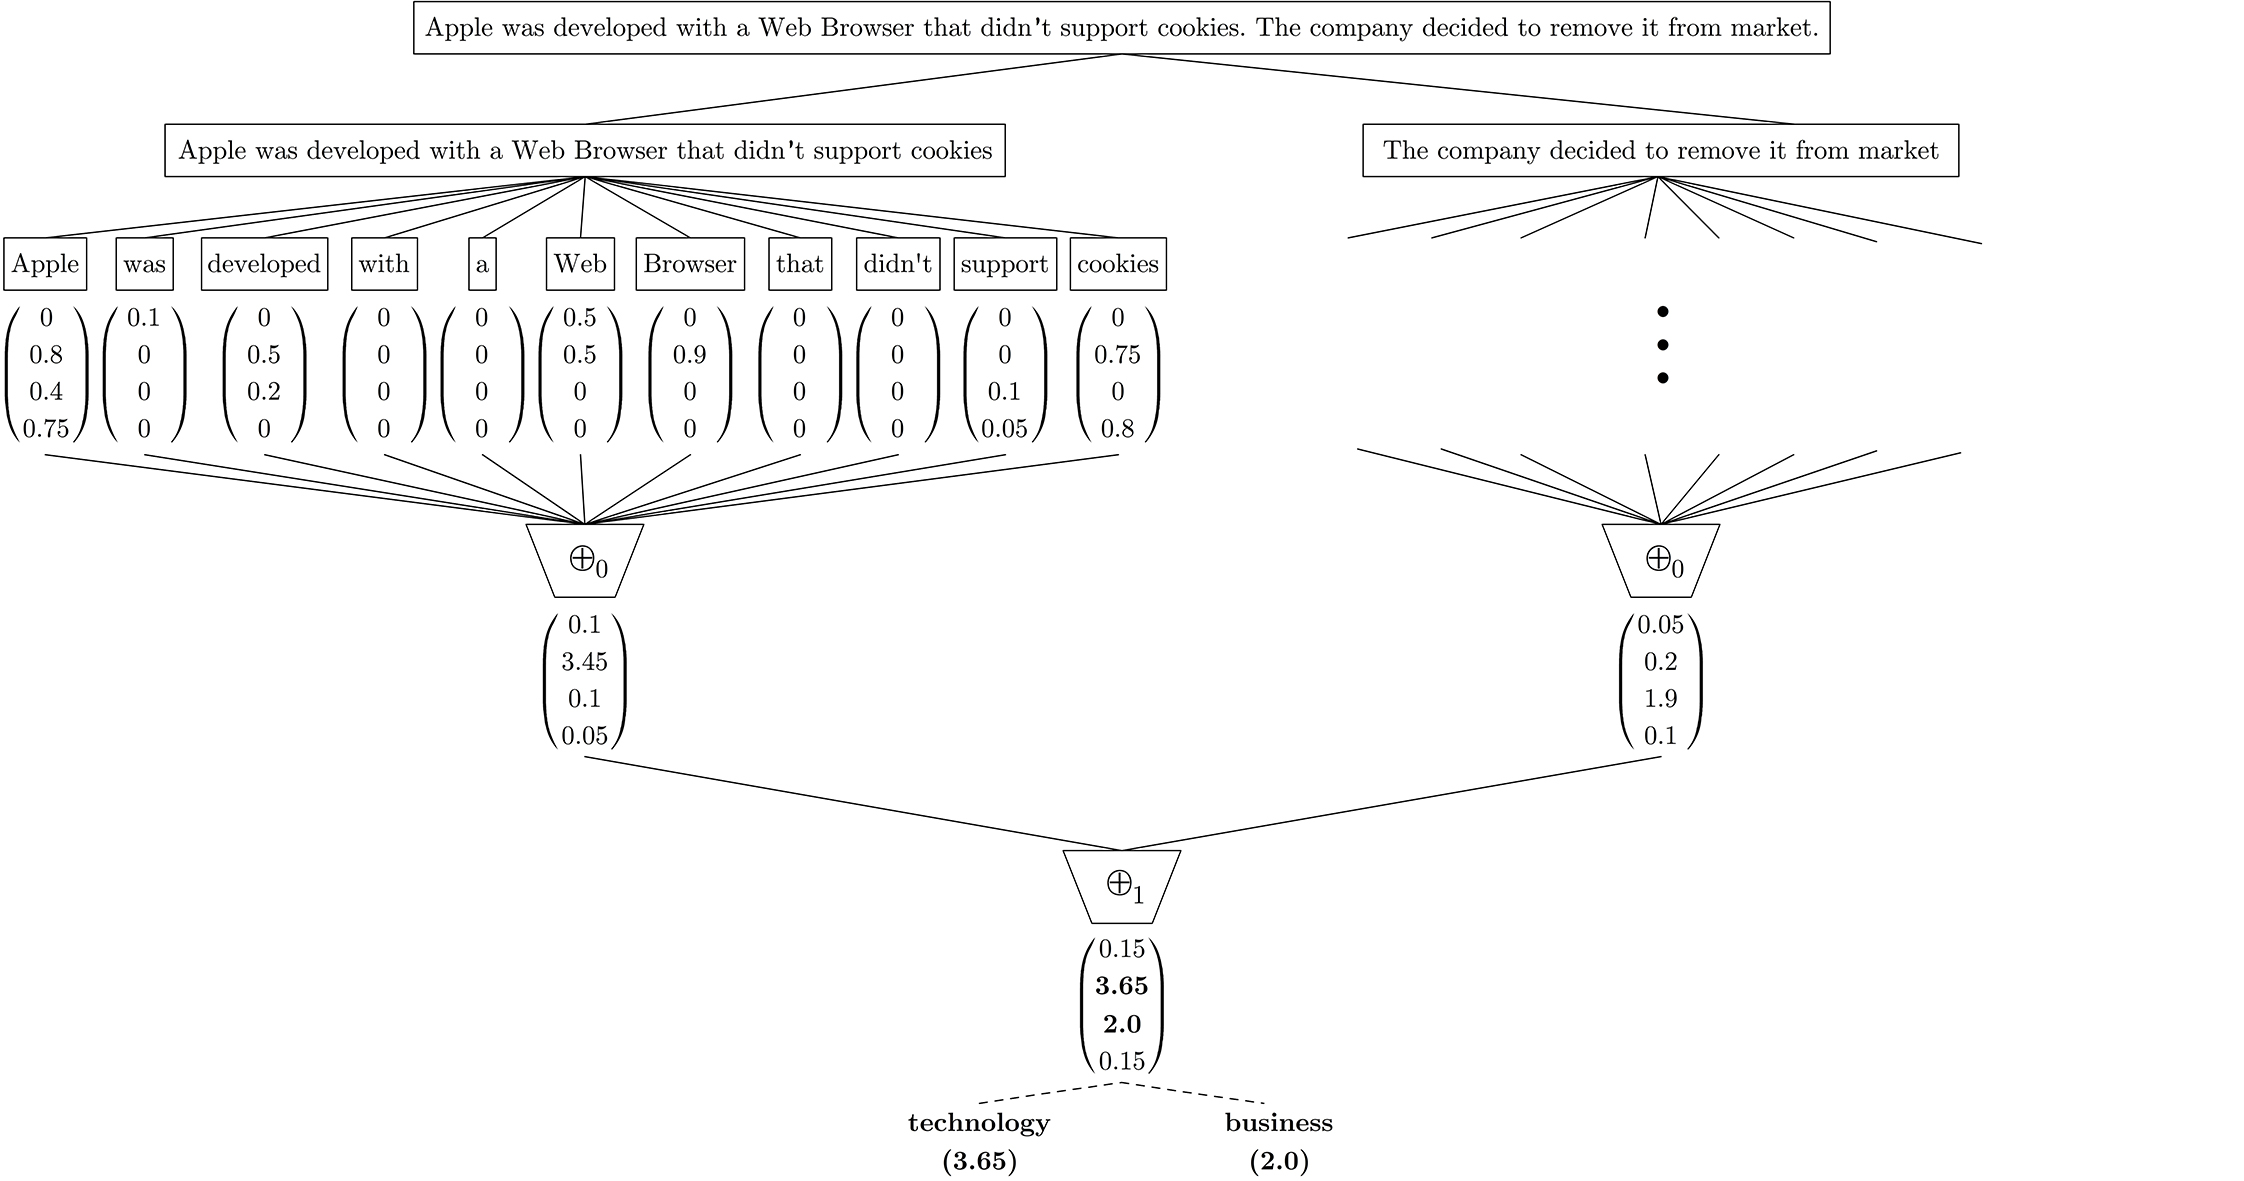
\includegraphics[width=190mm]{images/mapreduce-ss3}}
    \caption{Ejemplo del proceso de clasificación para el documento hipotético \emph{``Apple was developed with a Web Browser that didn't support cookies. The company decided to remove it from market''}.
    Al comienzo, este documento se divide en dos oraciones y luego cada oración a su vez se divide en palabras individuales.
    En este punto, se utiliza la función $gv$ sobre estas palabras individuales para obtener sus \emph{vectores de confianza}.
    Luego, estos vectores se reducen utilizando un operador especial, $\oplus_0$, a dos nuevos vectores de confianza a nivel oración, $\langle 0.1, 3.45, 0.1, 0.05\rangle$ y $\langle 0.05, 0.2, 1.9, 0.1\rangle$ para la primera y segunda oración, respectivamente.
    A su vez, estos dos últimos vectores también se reducen utilizando otro operador, $\oplus_1$, que en este caso es el operador de suma, a un único \emph{vector de confianza} final para todo el documento, $\langle 0.15, 3.65, 2.0, 0.15\rangle$.
    Finalmente, utilizando alguna política sobre este vector de confianza final, se selecciona la o las clases a ser signadas; en este ejemplo, se selecciona a \emph{tecnología} (\emph{technology}), por tener el valor de confianza más alto, y también a \emph{negocios} (\emph{business}) porque su valor está ``lo suficientemente cerca'' al de \emph{tecnología}.}
    % \caption{Classification process for a hypothetical example document ``Apple was developed with a Web Browser that didn't support cookies. The company decided to remove it from the market''.
% In the first stage, this document is split into two sentences (for instance, by using the dot as a delimiter) and then each sentence is also split into single words.
% In the second stage,  \emph{global values} are computed for every word to generate the first set of \emph{confidence vectors}.
% Then all of these word vectors are reduced by the $\oplus_0$ operator to sentence vectors, $(0.1, 3.45, 0.1, 0.05)$ and $(0.05, 0.2, 1.9, 0.1)$ for the first and second sentence respectively.
% After that, these two sentence vectors are also reduced by another operator ($\oplus_1$, which in this case is the addition operator) to a single \emph{confidence vector} for the entire document, $(0.15, 3.65, 2.0, 0.15)$.
% Finally, a policy is applied to this vector to make the classification ---which in this example was to select \emph{technology}, the category with the highest value, and also \emph{business} because its value was ``close enough'' to \emph{technology}'s.}
    \label{fig:mapreduce}
\end{figure*}


\

Ahora que ya hemos introducido los elementos y terminología necesaria, estamos listos para describir el proceso de clasificación, el cual puede pensarse como un proceso de dos fases, ilustrado con un ejemplo en la \autoref{fig:mapreduce}.
La primera fase comienza dividiendo el documento de entrada en múltiples bloques, luego cada bloque a su vez se divide sucesivamente en unidades más pequeñas hasta llegar a las palabras individuales.\footnote{Utilizaremos palabras aquí para simplificar la explicación, pero como se vio en la \autoref{sec:tipo-termino}, en principio se podría utilizar cualquier tipo de término, dependiendo de la tarea a resolver.} ---\emph{e.g.} dividir el documento en párrafos, párrafos en oraciones y oraciones en palabras.
Al finalizar esta fase, la entrada, previamente ``plana'', se ha convertido en una jerarquía de distintos niveles de bloques.
Así, diremos que las palabras están en el nivel 0 de la jerarquía, las oraciones en el nivel 1, los párrafos en el nivel 2, y así sucesivamente.
En la segunda fase, la función $gv$ se aplica a cada palabra para obtener los \emph{vectores de confianza} de ``nivel 0'', los cuales serán luego reducidos a \emph{vectores de confianza} de un siguiente nivel utilizando un operador especial para cada nivel, llamado \emph{operador de resumen}, $\oplus_0$.
Este proceso de reducción por operadores de resumen se propaga recursivamente a los bloques de nivel superior, hasta obtener un único \emph{vector de confianza} para toda la entrada.
Finalmente, la clasificación propiamente dicha se realiza aplicando alguna política para seleccionar las o la clase adecuada en base a los valores de este único \emph{vector de confianza} ---por ejemplo, seleccionando la clase con el máximo valor.
Notar que los \emph{operadores de resumen}, $\oplus_j$, se denotan utilizando un subíndice $j$, esto indica que cada nivel podría utilizar una operación diferente ---\emph{e.g.} $\oplus_0$ podría ser una suma de vectores, $\oplus_1$ el promedio (\emph{mean pooling}), $\oplus_2$ el máximo (\emph{max pooling}), y así. Más aún, no sólo operadores simples sino cualquier método, algoritmo o función, de la forma $f:2^{\mathbb{R}^n}\mapsto\mathbb{R}^n$, podría usarse como un \emph{operador de resumen}.
% Now that the needed basic definitions and terminology have been introduced, we are ready to describe the overall classification process, which is illustrated with an example in \autoref{fig:mapreduce}.
% Classification can be thought of as a 2-phase process.
% The first phase starts out by splitting the given input (usually a single document) into multiple blocks, then each block is in turn repeatedly divided into smaller units until words are reached.
% At the end of this phase, we have converted the previously ``flat'' input into a hierarchy of blocks.
% In practice, a document will be typically divided into paragraphs, paragraphs into sentences and sentences into words.
% Additionally, we will say that words are at level 0 in this hierarchy, sentences at level 1, paragraphs at level 2, and so on.
% In the second phase, the $gv$ function is applied to each word to obtain the level 0 \emph{confidence vectors}, which then are reduced by means of a \emph{summary operator} to generate the next level's \emph{confidence vectors}.
% This reduction process is recursively propagated up to higher-level blocks until a single \emph{confidence vector} is generated for the whole input.
% Finally, the actual classification is performed based on the values of this single \emph{confidence vector} ---some policy must be used, e.g. the category with the maximum value.
% Note that in the example shown in \autoref{fig:mapreduce}, \emph{summary operators} are denoted by $\oplus_j$, where $j$ denotes the level, to highlight the fact that each level (e.g. words, sentences, etc.) could have a different \emph{summary operator}
% ---for instance, $\oplus_0$ could be addition, $\oplus_1$ maximum (i.e. max pooling), $\oplus_2$ average (i.e. mean pooling), etc. Moreover, any function of the form $f:2^{\mathbb{R}^n}\mapsto\mathbb{R}^n$ could be used as a \emph{summary operator}.


\begin{figure}[t!] % [t]op; [h]ere; [p]age; [b]ottom; [r]ight; [l]eft
    \centering
    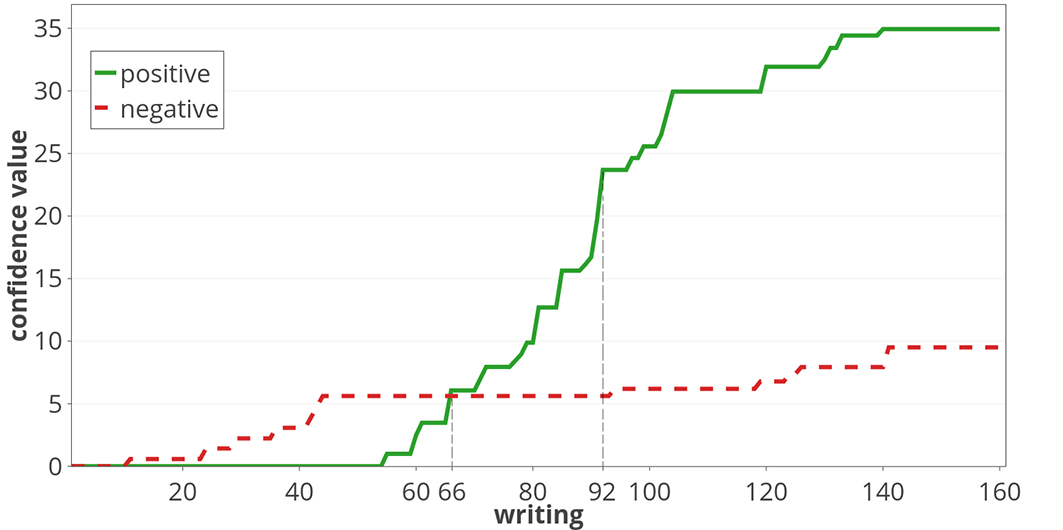
\includegraphics[width=120mm]{images/test_subject9579_writings}
    \caption{Variación del \emph{valor de confianza} positivo y negativo a lo largo del tiempo, hasta el momento. El tiempo se mide en publicaciones (writings) por lo que el gráfico seguiría creciendo a medida que el usuario escriba nuevas publicaciones.}
    % \caption{subject 9579's positive and negative confidence value variation over time. Time is measured in writings and it could be further expanded as more writings are created by the subject over time.}
    \label{fig:subject9579_writings}
\end{figure}

Vale la pena mencionar que este proceso le permite al clasificador explicar, visualmente, las razones detrás de la clasificación si, por ejemplo, en el documento de entrada se colorea cada bloque con una intensidad proporcional a su respectivo valor de confianza ---como se ilustrará con un ejemplo al final de la \autoref{sec:analysisAndDiscussion}.
Además, el clasificador podrá trabajar incrementalmente siempre que el \emph{operador de resumen} elegido para el último nivel pueda calcularse incrementalmente
---como es el caso con las operaciones de agregación más comunes, como la suma, la multiplicación, el máximo o incluso el promedio.\footnote{En el caso del promedio, sería necesario almacenar, además de la suma de los \emph{vectores de confianza} leídos hasta el momento, el número de vectores leídos.}
Por ejemplo, supongamos que más adelante se agrega una nueva oración al ejemplo mostrado en la \autoref{fig:mapreduce}, como $\oplus_1$ es la suma de vectores, en lugar de procesar nuevamente todo el documento, sólo necesitaríamos procesar la nueva oración para sumar su \emph{vector de confianza} a nuestro antiguo vector ya calculado, $\langle 0.15, 3.65, 2.0, 0.15\rangle$ ---obteniendo así el mismo vector final que obtendríamos si procesáramos toda la entrada nuevamente.
% It is worth mentioning that with this simple mechanism it would be fairly straightforward to justify when needed, the reasons of the classification by using the values of \emph{confidence vectors} in the hierarchy, as will be illustrated with a visual example at the end of \autoref{sec:analysisAndDiscussion}.
% Additionally, the classification is also incremental as long as the \emph{summary operator} for the highest level can be computed in an incremental fashion
% ---which is the case for most common aggregation operations such as addition, multiplication, maximum or even average.\footnote{In case of average it would be necessary to store, in addition to a vector with the sum of all previous \emph{confidence vectors}, their number.}
% For instance, suppose that later on, a new sentence is appended to the example shown in \autoref{fig:mapreduce}.
% Since $\oplus_1$ is the addition, instead of processing the whole document again, we could update the already computed vector, $(0.15, 3.65, 2.0, 0.15)$, by adding it to the new sentence \emph{confidence vector}
% --- Note that this incremental classification, in which only the new sentence needs to be processed, would produce exactly the same result as if the process were applied to the whole document again each time.
Finalmente, otro aspecto importante de este enfoque incremental es que, dado que este \emph{vector de confianza} final mantiene un resumen de la entrada leída hasta el momento, realizar un seguimiento de \emph{cómo} este vector cambia con el tiempo, a medida que se procesen nuevos elementos, debería permitirnos derivar reglas sencillas y claras para decidir \emph{cuándo} el clasificador puede hacer una clasificación anticipada.
% Another important aspect of this incremental approach is that since this \emph{confidence vector} is a value that ``summarizes the past history'', keeping track of \emph{how} this vector changes over time should allow us to derive simple and clear rules to decide \emph{when} the system should make an early classification. %, as we will see in section \autoref{sec:analysisAndDiscussion}.
Por ejemplo, supongamos que necesitamos clasificar a un usuario de una red social como ``positivo'' o ``negativo'' en relación a algún riesgo,  en base a las publicaciones que va generando.
Además, supongamos que este usuario efectivamente está en riesgo y que el cambio de los valores de su \emph{vector de confianza} hasta el momento, y a lo largo del tiempo, es el mostrado en la \autoref{fig:subject9579_writings}.
% As an example of this, suppose we need to classify a social media user (i.e. a subject) as depressed (positive) or non-depressed (negative) based on his/her writings.
% Let us assume that this user is the subject 9579, he/she is depressed, and that the change of each \emph{confidence vector} component over time (measured in writings) is the one shown in \autoref{fig:subject9579_writings}.
Podríamos hacer uso de esta información temporal y dinámica para diseñar políticas que le permitan al clasificador decidir en qué momento clasificar a los sujetos como positivos.
Por ejemplo, una política podría ser ``clasificar al usuario como positivo cuando el valor positivo actual sea mayor al negativo'', en cuyo caso nuestro usuario se hubiera clasificado como positivo luego de que éste escribiese su publicación número 66.
Otra política, un poco más elaborada, podría tener en cuenta qué tan rápido crece el valor positivo en relación al negativo, clasificando al usuario como positivo cuando el crecimiento supere cierto umbral. Por ejemplo, con una política de este tipo, nuestro usuario podría haber sido clasificado como positivo luego de haber escrito su publicación número 92.
% Tenga en cuenta que también se podrían combinar múltiples políticas como veremos en la \autoref{sec:analysisAndDiscussion}.
% We could make use of this ``dynamic information'' to apply certain policies to decide when to classify subjects as depressed.
% For example, one of such a policy would be ``classify a subject as positive when the accumulated positive value becomes greater than the negative one'' ---in which case, note that our subject would be classified as depressed after reading his/her 66th writing.
% Another (more elaborated) policy could have taken into account how fast the positive value grows (the slope) in relation with the negative one, and if a given threshold was exceeded, classify subjects as depressed ---in such case our subject could have been classified as depressed, for instance, after reading his/her 92nd writing.
% Note that we could also combine multiple policies as we will see in \autoref{sec:analysisAndDiscussion}.



\subsubsection{Entrenamiento}
\label{sec:training_process}

En la subsección anterior se describió el proceso de clasificación, el cual se apoya sobre los \emph{vectores de confianza}, los que a su vez se generan inicialmente con la función $gv$, la cual nos da el \emph{valor global} de las palabras.
En esta sección se describe cómo se lleva a cabo el entrenamiento del clasificador, esto es, cómo hace SS3 para aprender el \emph{valor global} de las palabras (\emph{i.e.} aprende a calcular $gv(w,c)$) en base a los documentos del conjunto de entrenamiento.
Sin embargo, el cálculo efectivo de $gv(w,c)$ se pospondrá para la \autoref{sec:local_global_value}, ya que, como se verá allí, SS3 puede calcularlo completamente conociendo la frecuencia de cada palabra.

De este modo, el entrenamiento propiamente dicho se vuelve trivial, ya que sólo consiste en almacenar la frecuencia total que tiene cada palabra dentro de cada clase.
% puede calcularse completamente en base a la frecuencia de cada palabra en cada clase, el entrenamiento de modelos SS3 es prácticamente trivial ya que sólo necesitaríamos almacenar dichas frecuencias.
Esto es, el algoritmo de aprendizaje simplemente consiste en la utilización de un diccionario de pares palabra-frecuencia por cada clase, para almacenar dichas frecuencias, y la posterior actualización de los mismos, a medida que se leen nuevos documentos de entrenamiento ---\emph{i.e} las palabras nuevas se agregan al diccionario y las ya conocidas actualizan su frecuencia.
% This brief subsection describes the training process, which is trivial. Only a dictionary of term-frequency pairs is needed for each category.
% Then, during training, dictionaries are updated as new documents are processed ---i.e. unseen terms are added and frequencies of already seen terms are updated.

\vspace{5mm}

Notar que con este simple algoritmo de entrenamiento, SS3 no necesita almacenar todos los documentos ni volver a entrenar desde cero cada vez que se agregan nuevos documentos de entrenamiento, en su lugar, sólo se deben actualizar las frecuencias ya almacenadas utilizando los nuevos documentos disponibles.
En otras palabras, el entrenamiento también puede realizarse incrementalmente,\footnote{En principio, incluso hasta nuevas clases podrían agregarse dinámicamente.} lo que dentro del área del aprendizaje automático se conoce como \emph{online learning}.
% Note that with this simple training method there is no need neither to store all documents nor to re-train from scratch every time a new training document is added, making the training incremental.\footnote{Even new categories could be dynamically added.}
Además, no es necesario, como es usual, crear y calcular una matriz documento-término, ya que, en particular, el concepto de documento deja de tener sentido para el modelo y, en su lugar, cada clase es vista como una ``gran bolsa de palabras''.
%Esto a su vez, como sugieren los resultados experimentales, dota al modelo de cierta robustez ante el conocido problema de desbalance de clases ---ya que el número de documentos en cada clase es irrelevante en tanto la frecuencia relativa de las palabras dentro de ``cada bolsa'' sea representativa.
% , durante la clasificación, $gv$ puede calcularse dinámicamente en función de las frecuencias almacenadas en los diccionarios ---aunque, en caso de que sea necesario, siempre será posible crearla.
Finalmente, desde un punto de vista computacional, el costo del entrenamiento es muy bajo, ya que sólo involucra actualizar las frecuencias de cada término, es decir, sólo involucra operaciones de suma.
% Additionally, there is no need to compute the document-term matrix because, during classification, $gv$ can be dynamically computed based on the frequencies stored in the dictionaries ---although, in case we are working in an offline fashion and to speed up classification, it is still possible to create the document-term matrix holding the $gv$ value for each term.
% Finally, also note that training computation is very cheap since involves only updating term frequencies i.e only one addition operation is needed.


\subsection{Detalles Técnicos y Formalización}
\label{sec:formal_description}

En esta sección se formalizan las descripciones e intuiciones introducidas en las secciones anteriores, brindando los algoritmos correspondientes y examinando el cálculo efectivo de $gv$.
% This section presents more formally the general and intuitive description given in the previous section.

\subsubsection{Algoritmos de Clasificación y Entrenamiento}
% \subsection{Classification and Training}

\begin{algorithm}[t!]
\small
\caption{\small Algoritmo de clasificación de SS3.
$MAX\_NIVEL$ es una constante que almacena el nivel máximo de jerarquía utilizado al particionar la entrada. Por ejemplo, debería usarse $MAX\_NIVEL=3$ cuando se trabaje con la partición ``párrafo- oración-palabra''.
La función \textproc{Map} aplica \textproc{Clasificar-a-Nivel}($bloque$, $n-1$) a cada $bloque$ en $bloques$ y devuelve la lista de vectores resultantes.
La función \textproc{Reduce} reduce los vectores en $bloques\_vcs$ a un solo vector utilizando el \emph{operador de resumen} $\oplus_{n-1}$}
\label{alg:classification}
\begin{algorithmic}
\Statex
\Function{Clasificar}{$texto$} \Returns un conjunto de etiquetas de clases
	\State \Input $texto$, una secuencia de símbolos
	\State \LocalVariables $\overrightarrow{c}$, el \emph{vector de confianza} del documento
	\State
	\State $\overrightarrow{c} \gets$ \Call{Clasificar-a-Nivel}{$texto$, $MAX\_NIVEL$}
	\State
	\State \Return una o más clases seleccionadas en base a $\overrightarrow{c}$ según alguna política
\EndFunction
\Statex \hrulefill
\Function{Clasificar-a-Nivel}{$texto$, $n$} \Returns un \emph{vector de confianza}
	\State \Input $texto$, una secuencia de símbolos
	\State \LocalVariables $bloques$, una lista de bloques de texto
	\State \localvarsindent $bloques\_vcs$, lista de \emph{valores de confianza} de los bloques
	\State
	\If{$n$ == 0} \Comment es decir, si $texto$ es ``indivisible'' (\emph{e.g.} $texto=$ una palabra)
		\State \Return $gv(texto)$
% 		\State \Return \Call{Valor-Global}{$texto$}
	\Else
		\State $bloques \gets$ dividir $texto$ en bloques más pequeños \Comment \emph{i.e.} en bloques de nivel $n$
		\State $bloques\_vcs \gets$ \Call{Map}{}(\Call{Clasificar-a-Nivel}{}, $bloques$, $n - 1$)
		\State \Return \Call{Reduce}{}(\Call{$\oplus_{n-1}$}{}, $bloques\_vcs$)
	\EndIf
\EndFunction
\end{algorithmic}
\end{algorithm}

En el \autoref{alg:classification} se presenta el algoritmo de clasificación general que lleva a cabo el proceso ilustrado anteriormente en la \autoref{sec:classification_process}.
% In \autoref{alg:classification} is shown the general multi-label classification algorithm which carries out the process illustrated earlier in \autoref{sec:classification_process}.
Notar que este algoritmo se puede paralelizar masivamente, ya que sigue de manera natural el modelo de programación \emph{MapReduce}~\cite{dean2008} para \emph{big data}, lo que, en principio, le daría al modelo la capacidad de procesar y manejar efectivamente grandes volúmenes de datos.
% Note that this algorithm can be massively parallelized since it naturally follows the Big Data programming model \emph{MapReduce}~\cite{dean2008}, giving the framework the capability of effectively processing very large volumes of data. 

\begin{algorithm}[t!]
\small
\caption{\small Algoritmo de entrenamiento de SS3, implementado aquí por el procedimiento \textproc{Aprender}, el cual puede volverse a ejecutar cuando nuevos documentos de entrenamiento se vuelvan disponibles.}
\label{alg:training}
\begin{algorithmic}
\Statex
\Procedure{Aprender}{$documentos$}
	\State \Input $documentos$, una lista de documentos etiquetados con su respectiva clase
	\State
	\For{$documento$ \In $documentos$}
		\State \Call{Aprender-Documento}{$documento$.TEXTO, $documento$.ETIQUETA}
	\EndFor
	\State
	\State \Call{Actualizar-Valores-Globales}{}() \Comment{este paso es opcional}
\EndProcedure
\Statex \hrulefill
\Procedure{Aprender-Documento}{$texto$, \emph{etiqueta}}
	\State \Input $texto$, la secuencia de palabras del documento
	\State \inputindent \emph{etiqueta}, la etiqueta de la clase a la que pertenece el documento
	\State
	\State DICCIONARIO $\gets$ el diccionario correspondiente a la clase de la \emph{etiqueta}
	\For{\emph{palabra} \In $texto$}
		\If{\emph{palabra} $\notin$ DICCIONARIO}
			\State agregar \emph{palabra} a DICCIONARIO
		\EndIf
		\State DICCIONARIO[\emph{palabra}] $\gets$ DICCIONARIO[\emph{palabra}]$ + 1$
	\EndFor
\EndProcedure
\end{algorithmic}
\end{algorithm}

En el \autoref{alg:training} se presenta el algoritmo de entrenamiento descrito informalmente en la sección anterior.
Notar que la línea que llama a la función \textproc{Actualizar-Valores-Globales}, la cual calcularía y actualizaría todos los valores globales dados por $gv$, sólo sería necesaria si quisiéramos precomputarlos y almacenarlos a modo de caché, por ejemplo, para evitar recalcularlos reiteradas veces durante la clasificación;
% In \autoref{alg:training} is shown the training process described earlier.
% Note that the line calling the \textproc{Actualizar-Valores-Globales} function, which calculates and updates all global values, is only needed if we want to construct the document-term matrix to work in the standard batch-like way.
de lo contrario, puede omitirse ya que, como mencionamos, durante la clasificación $gv$ podría calcularse dinámicamente en función de las frecuencias almacenadas en los diccionarios.
Finalmente, vale la pena mencionar que este algoritmo también podría paralelizarse siguiendo el modelo \emph{MapReduce} ---por ejemplo, el conjunto de entrenamiento podría dividirse en lotes, luego paralelamente se calculan las frecuencias dentro de cada lote y, finalmente, todas estas frecuencias locales se sumarían para obtener las frecuencias totales.
% Otherwise, it can be omitted since, during classification, $gv$ can be dynamically computed based on the frequencies stored in the dictionaries.
% It is worth mentioning that this algorithm could be easily parallelized by following the MapReduce model as well ---for instance, all training documents could be split into batches, then frequencies locally calculated within each batch, and finally, all these local frequencies summed up to obtain the total frequencies.


\subsubsection{Valor Global de una Palabra}
% \subsection{Local and Global Value of a Word}
\label{sec:local_global_value}

En esta sección finalmente abordaremos cómo podría hacer SS3 para aprender, efectivamente, el \emph{valor global} de las palabras en base a los documentos de entrenamiento.
% En otras palabras, abordamos cómo sería posible calcular $gv(w,c)$ en base a las frecuencias almacenadas durante el entrenamiento.
No obstante, y antes de comenzar, es necesario recordar que se espera que el modelo final sea confiable y transparente, capaz de explicar las razones detrás de la clasificación, como se explicó en la \autoref{sec:EC}.
Por lo tanto, SS3 debe ser interpretable para, de este modo, poder proveer explicaciones completamente fieles a lo que el modelo realmente computa\footnote{En tareas de riesgo, no es recomendable utilizar modelos de caja negra, no interpretables, ya que éstos requieren de técnicas especiales (tales como LIME, SHAP, Mean Decrease Accuracy o DeepLIFT) para generar las explicaciones. Dado que dichas explicaciones sólo brindan una \emph{aproximación} del funcionamiento real del modelo, su uso puede, entre otros problemas, ser peligroso~\cite{rudin2019stop}}.
Más precisamente, para que SS3 sea interpretable, se necesita que la valoración de las palabras por medio de este \emph{valor global} sea interpretable.
Sin embargo, uno de los principales desafíos de la interpretabilidad es que, dado que  pueden haber diferentes ideas de lo que constituye interpretabilidad, es necesario definirla de una manera específica al dominio abordado para luego integrar dicha definición directamente dentro de nuestro modelo~\cite{rudin2019stop}. 
Por lo tanto, es necesario definir qué constituya la interpretabilidad en el dominio abordado en este trabajo, esto es, la clasificación de texto para la DAR.

En la DAR, se espera que las explicaciones sean interpretables no para el científico computacional sino para un público no especializado ---por ejemplo, para un experto en la problemática abordada, como ser un especialista en la salud mental.
Así, en este trabajo, diremos que un modelo es interpretable si es capaz de valorar a las palabras de una forma que sea intuitiva para una público general, no especializado en las ciencias computacionales.
Más específicamente, inspirados en la forma en la que una persona típicamente le explicaría a otra en base a qué palabras decidió clasificar a un texto de cierta manera,\footnote{Por ejemplo, uno esperaría que la persona dirija su atención sólo a ciertas palabras, que funcionarían como ``palabras clave'', ignorando así la gran mayoría de las demás.} esperaremos que el modelo aprenda por un lado a identificar y valorar, con diferencia, a ciertas ``palabras clave'', y por el otro, filtrar todas las palabras que no sean necesarias, asignándole un valor casi nula a todas ellas ---similar a lo ejemplificado al comienzo de la \autoref{sec:classification_process}.
Por este motivo, no es posible utilizar un esquema de pesado de términos convencional, como ser \emph{tf-idf}, \emph{BM25} score, o los basados en \emph{DFR}, entre otros, ya que, en resumen, necesitamos una valoración que cumpla con estos dos requisitos: (a) que pondere cada término en relación a la decisión final, esto es, en relación a cada clase, no a cada documento;\footnote{Notar que los pesados de términos tradicionales fueron pensados para construir \emph{representaciones} de documentos, por lo que valoran un término en relación a un documento dado, no a una clase en particular.} y además (b) que dicha ponderación sea interpretable en el sentido ya mencionado.
De hecho, no conocemos un esquema de pesado que sea capaz de satisfacer estos dos aspectos en simultaneo, por lo que, en lo que resta de esta sección abordamos cómo sería posible calcular el \emph{valor global} de una palabra para lograrlo.
Esto es, desarrollaremos y propondremos una serie de ecuaciones para calcular $gv(w, c)$, en base a las frecuencias almacenadas durante el entrenamiento, intentando cumplir con ambos requerimientos.

\

Nuestro enfoque para calcular el \emph{valor global} busca superar los problemas que surgen de valorar las palabras únicamente basándonos en información local a cada clase. Para ello, primeramente, por medio de una función $lv(w,c)$ valoraremos la palabra únicamente en base a información local a cada clase, llamando a este valor como \emph{valor local}, pero luego combinaremos estos valores locales para obtener así el \emph{valor global} de la palabra, $gv(w,c)$.
% Our approach to calculating $gv$, as we will see later, tries to overcome some problems arising from the valuation of words only based on local information to a category. This is carried out by, firstly, computing a word \emph{local value} ($lv$) for every category, and secondly, combining them to obtain the \emph{global value} of the word in relation to all the categories.
Así, lo lógico es que el \emph{valor local} de una palabra $w$ en una clase $c$ sea proporcional a la probabilidad de que dicha palabra ocurra en textos de dicha clase, esto es, $lv$ debería ser alguna función tal que $lv(w, c)\propto P(w|c)$. Por lo tanto, definiremos a $lv$ como:
% More precisely, the \emph{local value} should be a function such that $lv(w, c) \propto P(w|c)$ i.e. the \emph{local value} of $w$ in $c$ should be proportional to the probability of $w$ occurring, given the category $c$. Therefore, $lv$ will be defined by:


\begin{equation}
\label{eq:lv-first}
lv(w, c) = \frac{P(w|c)}{P(w_{max}|c)}
\end{equation}


Donde $w_{max}$ denota la palabra más probable en la categoría $c$.
Notar que en lugar de definir $lv$ simplemente como $lv(w, c) = P(w|c)$, hemos decidido dividir dicha probabilidad por la probabilidad de la palabra más probable.
Esto produce dos efectos deseables:
(a) $lv$ está normalizado y la palabra más probable tendrá un valor de $1$ y, más importante aún,
(b) cada palabra se valora en relación a qué tan cerca esté su valor al de la más probable.
Lo interesante de este último punto es que las o la palabra más probable no dependerá de una clase en particular, sino del lenguaje en sí mismo. De hecho, en la práctica, la palabra más probable siempre será alguna de las \emph{palabras vacías} (tal como ``el'', ``la'', ``los'', ``las'', etc.) ya que por definición son palabras altamente frecuentes y cuya frecuencia está dada por el rol que desempeñan dentro del lenguaje en sí mismo, sin referir a la realidad extralingüística particular de cada clase.
Notar que con este simple ``truco'' de normalización, absolutamente todas las palabras se valoran en relación a un único elemento global e independiente de las clases particulares ---\emph{i.e.} las \emph{palabras vacías}. En otras palabras, hemos habilitado la posibilidad de \emph{comparar el valor local de una misma palabra a lo largo de las diferentes clases en ``igualdad de condiciones''} ---lo que en última instancia nos permitirá calcular su valor global.
% \footnote{Puede suceder que no sea exactamente la misma palabra para todas las clases, pero de ser ese el caso, serán \emph{palabras vacías} igualmente frecuentes, lo que a fines prácticos producirá los mismos resultados.}
%De hecho, en distintos experimentos realizados, la palabra más probable en todas las clases muy habitualmente resultó ser la palabra más frecuente del idioma inglés, ``the'', aunque para algunas clases, por ejemplo, resultaron ser ``be'', ``to'' o ``of'', la segunda, tercera o cuarta más frecuente del idioma.
% Notar que esto nos permite comparar el valor de una misma palabra a lo largo de las diferentes clases dado que su valor local en cada clase estará normalizado en relación a alguna \emph{palabra vacía}, las cuales siempre tendrán una probabilidad similar ya que su frecuencia está dada por el rol que desempeñan dentro del lenguaje en sí mismo, sin referir a la realidad extralingüística de cada clase en particular.
%, en gran medida, por la naturaleza propia del lenguaje en cuestión (Español, Inglés, etc.), y no por una clase en sí.
% Note that this allows us to compare words across different categories since their values are all normalized in relation to stop words, which should have a similar frequency across all the categories.\footnote{Note that we are assuming here that we are working with textual information in which there exist highly frequent elements that naturally have similar frequency across all categories (e.g. such as stop words).}

Sin embargo, antes de continuar con el cálculo del valor global, definiremos a $lv$ de una forma más general, ya que la definición dada en la \autoref{eq:lv-first} supone que la proporción $lv(w, c) \propto P(w|c)$ es directa, lo que no necesariamente tiene que cumplirse siempre. Así, agregaremos un parámetro, $\sigma$, que nos permitirá regular, de cierto modo, qué tan directa es la proporción $lv(w, c) \propto P(w|c)$, de la siguiente manera:
% However, our current definition of $lv$ implicitly assumes that the proportionality $lv(w, c) \propto P(w|c)$ is direct, which is not always true so we will define $lv$ more generally as follows:

$$lv_\sigma(w, c) = \left(\frac{P(w|c)}{P(w_{max}|c)}\right)^\sigma$$

\vspace{5mm}

Lo cual, después de estimar las probabilidades mediante \emph{estimación por máxima verosimilitud} (EMV) analítica, nos lleva finalmente a la siguiente definición, en términos de las frecuencias aprendidas durante el entrenamiento:
% Which, after estimating the probability, $P$, by an analytical \emph{Maximum Likelihood Estimation}(MLE) derivation, leads us to the actual definition:

\vspace{5mm}

\begin{equation}
\label{eq:lv-fr}
lv_\sigma(w, c) = \left(\frac{fr_{w,c}}{max\{fr_c\}}\right)^\sigma
\end{equation}

\vspace{5mm}

Donde $fr_{w, c}$ denota la frecuencia de $w$ en $c$ y $max\{fr_c\}$ la máxima frecuencia vista en $c$. De esta forma, el valor $\sigma\in(0, 1]$ es el primer hiperparámetro de nuestro modelo, denominado como ``suavidad'', y cuyo papel es doble ya que nos permite:
% Where $tf_{w,c}$ denotes the frequency of $w$ in $c$ and $max\{tf_c\}$ the maximum frequency seen in $c$. The value $\sigma  \in (0, 1]$ is the first hyper-parameter of our model, called ``smoothness'', and whose role is twofold:
\begin{itemize}
    \item Controlar qué tan rápido crecerá el \emph{valor local} de una palabra en relación a qué tan cerca esté su frecuencia a la de la más probable ---\emph{e.g.} cuando $\sigma = 1$, el crecimiento será lineal. %proporcional a $P(w|c)$.
    % \item Control how fast grows the \emph{local value} of a word in relation to how close it is to the most probable one; e.g. when $\sigma=1$, $lv$ grows linearly proportional to $P(w|c)$.
    \item Controlar ``la suavidad'' de la distribución de las palabras, que de lo contrario, según la ley empírica de Zipf \cite{zipf1949human, powers1998applications}, tendrá un grupo extremadamente pequeño de palabras muy frecuentes eclipsando a las importantes.
    % \item Control the smoothness of the distribution of words which otherwise, by the empirical Zipf's law \cite{zipf1949human, powers1998applications}, will have a very small group of highly frequent words overshadowing important ones.
\end{itemize}

\begin{figure}[t]
    \begin{subfigure}{0.5\textwidth}
        \centering
        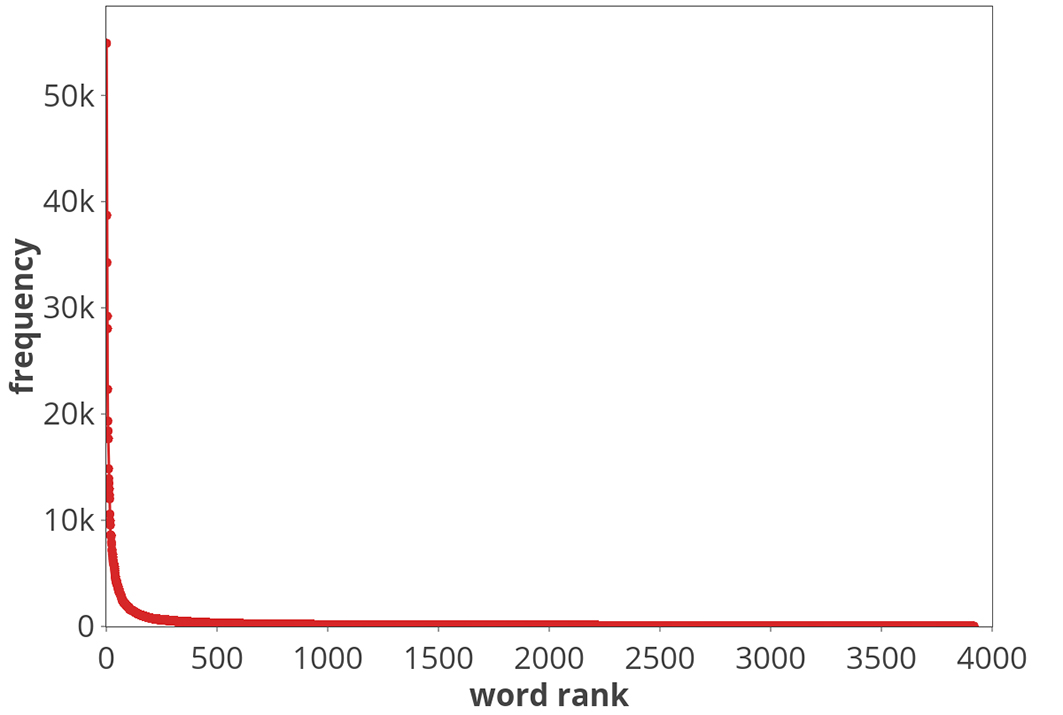
\includegraphics[width=90mm]{images/word-fr}
        \caption{}
        \label{fig:sigma_a}
    \end{subfigure}
    \begin{subfigure}{0.5\textwidth}
        \centering
        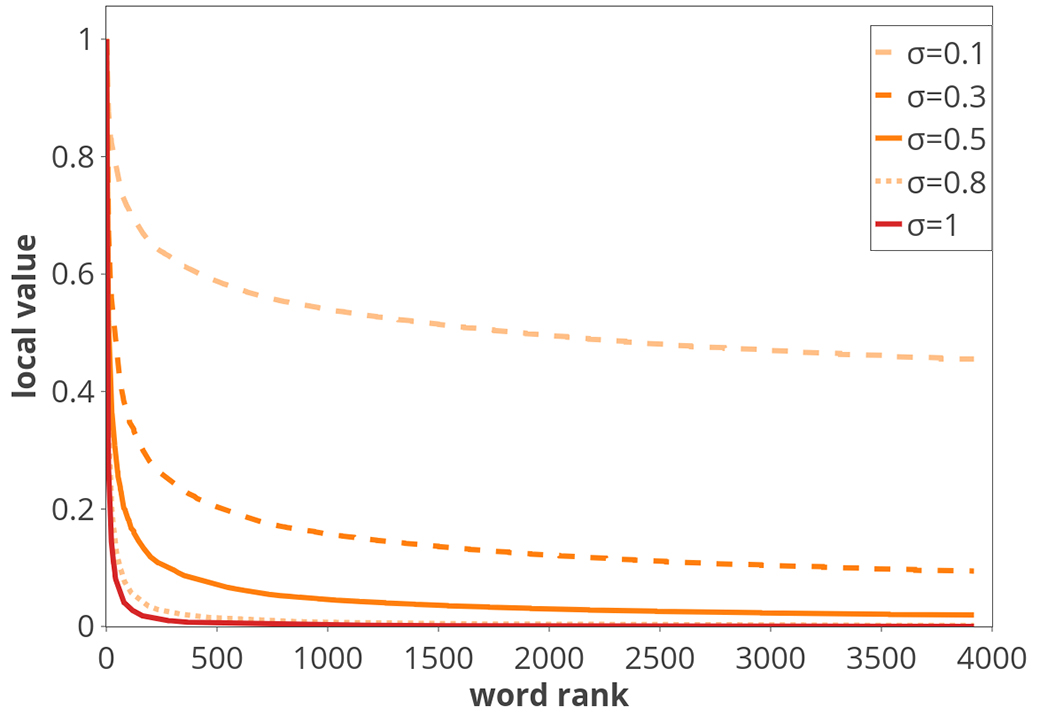
\includegraphics[width=90mm]{images/sigmas}
        \caption{}
    \end{subfigure}
\caption{
    (a) Curva con la distribución de la frecuencia de las palabras.
    (b) Curva con la distribución del \emph{valor local} de las palabras para cinco valores distintos de $\sigma$: $1$, $0.8$, $0.5$, $0.3$ y $0.1$.
    Las abscisas representan el ranking de las palabras individuales ordenadas por frecuencia en (a) y por valor local en (b).
    Notar que cuando $\sigma = 1$ (línea roja en (b)), la distribución de los \emph{valores locales} coincide exactamente, en forma, con la distribución de las frecuencias en bruto en (a). Sin embargo, a medida que el valor de $\sigma$ disminuye, la curva ``se suaviza'', haciendo que la brecha entre los valores más altos y más bajos se reduzca.
    % word-\emph{local value} diagram for 5 different values of $\sigma$: 1, 0.8, 0.5, 0.3 and 0.1.
    % The abscissa represents individual words arranged in order of frequency.
    % Note that when $\sigma=1$, $lv_1$ (red line) matches the shape of the raw frequency (the actual word distribution), however, as $\sigma$ decreases, the curve becomes smoother; reducing the gap between the highest and the lowest values.
}
\label{fig:sigma}
\end{figure}

Ambos aspectos se ilustran con un ejemplo en la \autoref{fig:sigma}.\footnote{En la práctica, normalmente los valores de $\sigma$ que nos han producido mejores resultados son los cercanos a $0.5$, lo que equivaldría, aproximadamente, a aplicarle la raíz cuadrada a la \autoref{eq:lv-first}.}
% These two items are illustrated with an example in \autoref{fig:sigma} ---a good value for $\sigma$ should be around 0.5, which would be approximately equivalent to taking the square root of the \autoref{eq:lv-first}.

\vspace{5mm}

Ahora que hemos definido una forma para calcular el \emph{valor local} de una palabra en las distintas clases, estamos listos para definir cómo combinar dichos valores para obtener su \emph{valor global}. Así, de forma general, definiremos a $gv(w,c)$ como $lv(w,c)$ regularizado por dos pesos especiales que capturan información global, $sig$ y $san$ , del siguiente modo:
% Now that we are able to compute word \emph{local values}, we are going to define its \emph{global value} based on them, as follows:

\begin{equation}
gv(w, c) = lv_\sigma(w, c)\times sig_{\lambda}(w, c)\times san_\rho(w, c)
\label{eq:gv}
\end{equation}

Donde $\lambda, \rho \in \mathbb{R}^+$ son los otros dos hiperparámetros del modelo, referidos como ``significancia'' y ``sanción'' respectivamente, y donde $sig$ y $san$ son dos funciones que, consultando el valor local de esa misma palabra $w$ en las otras clases, resaltarán o disminuirán su valor local en la clase dada $c$.
Más precisamente, $sig$ debería intentar capturar la ``significancia'' o importancia que tiene $w$ en $c$ observando su valor local en las otras clases, mientras que $san$ debería sancionar el valor final de $w$ en relación al número de clases para las cuales finalmente resultó importante, según $sig$.
% Where $sg$ and $sn$ are functions of the form $f:W\times C\mapsto [0, 1]$.
% As we will see, the former decreases $lv$ in relation to the global significance of $w$, and the latter sanctions it, in relation to the number of categories for which $w$ is significant.
% Additionally, the values  $\lambda, \rho \in \mathbb{R}^+$ referred to as ``significance'' and ``sanction'' respectively, are the other two hyper-parameters of our model.

\vspace{5mm}

De este modo, para que $sig(w, c)$ pueda reflejar correctamente la importancia de una palabra, $w$, con respecto a una clase, $c$, debería ser alguna función tal que:
(a) devuelva un valor cercano a $1$ cuando $lv(w, c)$ sea significativamente mayor que $lv(w, c_i)$ para las otras clases $c_i$; y a la inversa,
(b) devuelva un valor cercano a $0$ cuando sus \emph{valores locales} en las distintas clases sean similares entre sí, esto es, cuando $lv(w, c_i)$ sea similar para las distintas clases $c_i$.
Por ejemplo, $lv(\text{\emph{`el'}},c_i)$ será similarmente alto para todas las clases $c_i$, mientras que $lv(\text{\emph{`pan'}}, \text{alimentos})$ será probablemente mayor que $lv(\text{\emph{`pan'}}, c_i)$ para la mayoría de las otras clases; por lo tanto, $sig(\text{\emph{`el'}},c_i)$ debería devolvernos un valor cercano a $0$ mientras que $sig(\text{\emph{`pan'}}, \text{alimentos})$ cercano a $1$.
En general, podríamos modelar este comportamiento utilizando cualquier función sigmoide:
% In order to represent the significance of a word, $w$, with respect to a category, $c$, $sg(w, c)$ should be a function such that:
% (a) it outputs a value close to 1 when $lv(w, c)$ is significantly greater than $lv(w, c_i)$, for most other categories $c_i$; and
% (b) it outputs a value close to 0 when all $lv(w, c_i)$ are close to each other, for all $c_i$.
% For instance, $lv($`$the$'$, c_i)$ probably will be a similarly large value for all categories $c_i$, whereas $lv($`$bread$'$, food)$ probably will be greater than most  $lv($`$bread$'$, c_i)$, for other categories; hence $sg($`$the$'$, c_i)$ should be close to 0 and $sg($`$bread$'$, food)$ close to 1.
% In general, we could model this behavior by using any sigmoid function, as follows:


$$sig_{\lambda}(w, c) = sigmoide\left(lv(w, c) - \widetilde{LV}_w, \ \lambda\times MAD_w\right)$$

Tal que:
\begin{enumerate}
    \item[(I)] $sigmoide(d, l)\approx 1$ si $d\geq l$; y
    \item[(II)] $sigmoide(d, l)\approx 0$ si $d\leq0$.
\end{enumerate}

Donde $LV_w = \{lv(w, c_i) | c_i\in C\}$, es decir, el conjunto con todos los  \emph{valores locales} de $w$ en las distintas clases;
$\widetilde{LV}_w$ denota la mediana de $LV$;
$MAD_w = mediana(|lv(w,c_i)-\widetilde{LV}_w|)$, es decir, la \emph{Desviación Mediana Absoluta}\footnote{MAD, del inglés, Median Absolute Deviation.} de $LV_w$.
% Where $LV_w = \{lv(w, c_i) | c_i\in C\}$ i.e. the set of all \emph{local values} of $w$;
% $\widetilde{LV}_w$ denotes the median of $LV$;
% $MAD_w = median(|lv(w,c_i)-\widetilde{LV}_w|)$ i.e. the \emph{Median Absolute Deviation} of $LV_w$.
Notar que el hiperparámetro $\lambda$
% \footnote{si $\lambda$ es aproximadamente cercano a $1.4826$, entonces $\lambda\cdot MAD_w$ es aproximadamente igual a la \emph{desviación estándar} de $LV_w$, por lo tanto, $\lambda\approx 3\times1.4826$ podría ser un buen valor inicial para $\lambda$, siempre que $LV_w$ tenga una distribución normal.}
% Additionally, note that the hyper-parameter $\lambda$\footnote{
    % if $\lambda$ is approximately close to 1.4826, then $\lambda\cdot MAD_w$ is approximately equal to the \emph{standard deviation} of $LV_w$, thus perhaps setting $\lambda \approx 3\times1.4826$ would be a good value, as long as $LV_w$ has a normal distribution
% }
nos permite controlar qué tanto debe desviarse el \emph{valor local} de la mediana de \emph{valores locales} para ser considerado como significativo, es decir, mientras más cerca esté $lv(w, c)-\widetilde{LV}_w$ de superar a $\lambda\cdot MAD_w$, más cerca estará esta función $sigmoide$ de $1$.
% controls how far the \emph{local value} must deviate from the median to be considered significant i.e. the closer $lv(w, c)-\widetilde{LV}_w$ to $\lambda\cdot MAD_w$, the closer the $sigmoid$ to 1, and therefore, also the closer $sg_{\lambda}(w, c)$ to 1 ---which is the desired behavior.

Así, en particular, y sin perdida de generalidad, utilizaremos a la función sigmoide $tanh$ para definir a $sig$ como se definió arriba, cumpliendo con las propiedades allí mencionadas, del siguiente modo:
% In particular, we have decided to use $tanh$ as the $sigmoid$ function, hence $sg$ is defined by:

\begin{equation}
    sig_{\lambda}(w, c) = \frac{1}{2}\times tanh\left(4\times\frac{lv(w, c) - \widetilde{LV}_w}{\lambda\times MAD_w} - 2\right) + \frac{1}{2}
\end{equation}

\vspace{5mm}

Finalmente, necesitamos definir a $san$, la función de sanción, que disminuirá proporcionalmente el \emph{valor global} de una palabra en relación al número de clases para las cuales es significativa, según $sig$. Por lo tanto, $san$ debería ser una función tal que: (a) cuando $w$ sea significativo para una sola clase $c$, \emph{i.e.} cuando $sig_{\lambda} (w, c)\approx 1$ para un único $c$,  $san(w , c)$ debe ser igual a $1$; (b) cuanto mayor sea el número de clases en las que $w$ es significativa, menor debe ser el valor de $san(w, c)$. Por lo tanto, sin pérdida de generalidad, definiremos a $san$ como:
% Finally, we need to define $sn$, the sanction function, which will proportionally decrease the \emph{global value} of $w$, in relation to the number of categories for which $w$ is significant. Hence $sn$ should be a function such that: (a) when $w$ is significant (i.e. $sg_{\lambda}(w, c) \approx 1$) to only one category $c$, $sn(w, c)$ should be equal to 1; (b) the greater the  number of categories $w$ is significant to, the lower the value of $sn(w, c)$. Therefore, we have defined $sn$ by:

\begin{equation}
\label{eq:san}
    san_\rho(w, c) = \left(\frac
        {|C| - \left(\hat{C}_{wc} + 1\right)}
        {\left(|C|-1\right)\left(\hat{C}_{wc} + 1\right)}
    \right)^\rho
\end{equation}

% \begin{equation}
% \label{eq:san}
%     san_\rho(w, c) = \left(-\frac
%         {\hat{C}_{wc}}
%         {|C|-1} + 1
%     \right)^\rho
% \end{equation}

% \begin{equation}
% \label{eq:san}
%     san_\rho(w, c) = \left(-\frac
%         {\hat{C}_{wc}}
%         {|C|-1} + 1
%     \right)^\rho
% \end{equation}


Donde $|C|$ denota el número de clases y, 
$$\hat{C}_{wc} = \sum_{c_i\in C-\{c\}}sig_{\lambda}(w, c_i)$$
% Where $|C|$ denotes the number of categories and,
% $$\hat{C}_{wc} = \sum_{c_i\in C-\{c\}}sg_{\lambda}(w, c_i)$$


En palabras, $\hat{C}_{wc}$ es igual a la suma de ``la importancia'' de $w$ en todas las clases excepto $c$.
Notar que la \autoref{eq:san} se comporta de la manera deseada, por ejemplo,
cuando $w$ sea significativo para casi todas las clases, tendremos que $\hat{C}_{wc}\approx |C|-1$, y por lo tanto $san(w, c)\approx 0$, mientras que cuando $w$ sea significativo para una sola clase, $c$, se tendrá que $\hat{C}_{wc} = 0$, y por lo tanto $san(w, c) = 1$.
% i.e. $\hat{C}_{wc}$ is equal to the summation of $sg_{\lambda}(w, c_i)$ for all categories in $C$ except $c$.
% Note that, for instance, when extreme cases are met, \autoref{eq:san} behaves properly;
% namely, when $w$ is significant to almost all categories, $\hat{C}_{wc}\approx |C|-1$, and thus $sn(w, c)\approx 0$;
% and when $w$ is significant to only one category, $c$, $\hat{C}_{wc} = 0$, and thus $sn(w, c)= 1$.
Finalmente, notar que el hiperparámetro $\rho$ nos permite controlar qué tan severa es la sanción en relación al número de clases para las cuales la palabra es significativa.
% The hyper-parameter $\rho$ controls how severe the sanction is, in proportion to the number of significant categories.\footnote{
%     setting $\rho\approx 1$ probably is a good starting point, although we can adjust this value in relation to how overlapped categories are.
% }

\vspace{5mm}

Antes de concluir con esta sección, creemos conveniente introducir un ejemplo sencillo para ilustrar cómo el \emph{valor global} puede interpretarse efectivamente, según lo hemos definido en la \autoref{eq:gv}, como un porcentaje de su \emph{valor local} ($lv$), dado por su importancia ($sig$) y una sanción regularizadora ($san$). Así, supongamos que se tienen las siguientes tres clases $C=\{\text{\emph{alimentos}}, \text{\emph{tecnología}}, \text{\emph{negocios}}\}$, luego:
% To conclude this section, let us introduce a simple example to illustrate how the \emph{global value} is a percentage of its \emph{local value} given by its significance ($sg$) and sanction ($sn$). Suppose we have the following three categories $C = \{f, t, b\}$ for $food$, $tech$, and $business$ respectively, then:

\begin{itemize}
    \item {
        Para las \emph{palabras vacías} tendríamos, siendo $c$ cualquiera de las clases, casos similares al siguiente:
        % For stopwords, like `the', we would have, regardless of the category $c\in C$, something like:

        \vspace{5mm}

        \begin{tabular}{l@{}l}%p{0.5\linewidth}}
            $gv($`$el$'$, c)$  & $= lv($`$el$'$, c)\times sig($`$el$'$, c)\times san($`$el$'$, c)$\\
                            & $= lv($`$el$'$, c)\times 0.05\times 1$\\
                            & $= lv($`$el$'$, c)\times 0.05$\\
                            & $= 0.92\times 0.05 = 0.04$
        \end{tabular}

        \vspace{5mm}

        Notar que si bien el \emph{valor local} de ``el'' es alto ($0.92$), su \emph{valor global} final resultó ser muy bajo ($0.04$), sólo un $5\%$ de su \emph{valor local}.
        Esto se debe al hecho de que el \emph{valor local} de ``el'' fue igualmente alto en todas las clases y, por lo tanto, según definición de $sig$, su importancia es cercana a nula ---en este caso, $sig($`$el$'$, c) = 0.05$. A su vez, como su importancia es nula en todas las clases, no se aplicó ninguna sanción ---$san($`$el$'$, c)=1$.
        % While the \emph{local value} of `the' is 0.92, its final \emph{global value} turned out to be 0.04 (5\% of its \emph{local value}).
        % This is due to the fact that $lv($`$the$'$, c)$ is similarly high for all categories, and by definition, the significance function should be close to 0 ---in this case, $sg($`$the$'$, c)= 0.05$.
    }
    \vspace{5mm}
    \item {
        Para palabras que sean principalmente significativas para una única clase, como podría ser, por ejemplo, `pan' para \emph{alimentos}, tendríamos casos similares a éste:
        % For a word that is mainly significant to a single category, in this case, `bread' to food, we would have something like:

        \vspace{5mm}
        
        \begin{tabular}{l@{}l}%p{0.5\linewidth}}
            $gv($`$pan$'$, \text{\emph{alimentos}})$ & $= lv($`$pan$'$, \text{\emph{alimentos}})\times sig($`$pan$'$, \text{\emph{alimentos}})$\\ 
            					& \ \ \ $\times san($`$pan$'$, \text{\emph{alimentos}})$\\
                                & $= lv($`$pan$'$, \text{\emph{alimentos}})\times 0.99\times 0.95$\\
                                & $= lv($`$pan$'$, \text{\emph{alimentos}})\times 0.94$\\
                                & $= 0.65\times 0.94 = 0.61$
        \end{tabular}
        
        \vspace{5mm}

        El \emph{valor global} terminó siendo casi idéntico a su \emph{valor local} ---siendo más exactos, un $94\%$ de éste. Esto se debe a que no sólo la palabra fue significativa para \emph{alimentos} ($ sig($`$pan$'$, \text{\emph{alimentos}})=0.99$), sino que, además, prácticamente no se le aplicó ninguna sanción ($san($`$pan$'$, \text{\emph{alimentos}})=0.95$) debido a que no fue significativa para casi ninguna otra clase.
        % The \emph{global value} is almost identical to its \emph{local value} (about 94\%). This is due to the word being significant ($sg\approx 1$) \emph{only} to food ($sn\approx 1$).
    }
    \vspace{5mm}
    \item {
        Para palabras que son significativas para más de una clase, tendríamos casos similares al siguiente:
        % For a word that is significant to more than a single category, we would have something like:

        \vspace{5mm}

        \begin{tabular}{l@{}l}%p{0.5\linewidth}}
            $gv($`$apple$'$, \text{\emph{tecnología}})$ & $= lv($`$apple$'$, \text{\emph{tecnología}})\times sig($`$apple$'$, \text{\emph{tecnología}})$\\
            					& \ \ \ $\times san($`$apple$'$, \text{\emph{tecnología}})$\\
                                & $= lv($`$apple$'$, \text{\emph{tecnología}})\times 0.85\times 0.6$\\
                                & $= lv($`$apple$'$, \text{\emph{tecnología}})\times 0.51$\\
                                & $= 0.7\times 0.51 = 0.35$
        \end{tabular}
        
        \vspace{5mm}

        En este caso, el \emph{valor global} terminó siendo un $51\%$ de su \emph{valor local}.
        Notar que si bien ``apple'' es bastante significativa para \emph{tecnología} ($sig($`$apple$'$, \text{\emph{tecnología}})=0.85$), también lo debe ser para alguna o algunas de las otras dos clases, \emph{alimentos} y/o \emph{negocios}, al menos en cierta medida, porque fue moderadamente sancionado ($san($`$apple$'$, \text{\emph{tecnología}})=0.6$).
        % In this case, the \emph{global value} ended up being about 51\% of its \emph{local value}.
        % Note that while `apple' is quite significant to $tech$ ($sg=0.85$), it must also be significant to some of the other categories, at least to a certain degree, because it is being moderately sanctioned ($sn=0.6$).
    }
\end{itemize}

Es interesante notar que SS3 aprenderá a ignorar las \emph{palabras vacías} automáticamente, ya que para ellas tendremos, por definición, que $gv(w, c)\approx0$, por lo que no necesitaríamos eliminarlas manualmente durante el preprocesamiento, como es habitual.
% It is worth mentioning that SS3 will learn to automatically ignore stop words since, by definition, $gv(w, c)\approx0$ for all of them.
% Therefore, there is no need to manually remove stop words.
De hecho, la eliminación de las \emph{palabras vacías} probablemente produzca un efecto negativo ya que, como se explicó luego de definir la \autoref{eq:lv-fr}, la valoración de todas las palabras se realiza, precisamente, usando a las \emph{palabras vacías} como punto común independiente de clases particulares ---lo que nos permite compararlas a lo largo de las distintas clases para obtener sus valores globales.
% Moreover, stop words removal could cause negative effects since in \autoref{eq:lv} we are implicitly evaluating words in terms of stop words.\footnote{\textcolor{blue}{That is, words are normalized over the frequency of the most probable one, which will always be a stop word.
% Note that the fact that stop words have a similar distribution across all the categories enables us to compute the $gv$ value of a word by comparing its $lv$ value across different categories.}}
No obstante, no hay nada en el modelo que nos impida utilizar cualquier otra técnica de preprocesamiento, tales como \emph{stemming} o \emph{lemmatization}.
% However, there is nothing in the model preventing us from using any other type of preprocessing, such as stemming, lemmatization, etc.

\

Finalmente, también es interesante mencionar que el clasificador \acf{MNB} puede verse como ``una instancia posible'' del modelo SS3. En concreto, una instancia en la que el valor global se redujera simplemente al valor local, definiendo a $gv$ como $gv(w, c) = lv(w, c) = log\ P(w|c)$ y a $\oplus_j = suma$, para todo $j$.\footnote{Al final de la \autoref{sec:mnb} del \autoref{cap2} se explicó la razón de este $log\ P(w|c)$ en \ac{MNB}.}
Sin embargo, esta instancia de SS3 no cumpliría efectivamente nuestros objetivos, ya que,
% A saber, como se tiene que $\sum_{w \in W} P(w|c) = 1$ por definición de probabilidad $P$, esto es, la suma de las probabilidades de todas las palabras deben ser 1, y dado que el número de palabras por clase es generalmente muy grande, los distintos valores $log\ P (w|c)$ terminan siendo extremadamente pequeños y muy similares entre sí (esto último debido al efecto del logaritmo) sin importar la palabras $w$.
de esta manera, la frecuencia local de una palabra en una clase pasaría a ser el único factor que determinase su valor. Así, ``palabra frecuente'' se volvería sinónimo de ``palabra valiosa'' y, por lo tanto, las palabras realmente valiosas se verían ocultas por simples palabras frecuentes, pero sin importancia ---como las \emph{palabras vacías}.
% Esto afecta tanto a la capacidad de describir qué palabras ayudaron a tomar la decisión como así también, por lo general, al desempeño del modelo ---otros tipos de modelos, tales como \ac{SVM} habitualmente superan a \ac{MNB}.
En resumen, el principal aspecto negativo con \ac{MNB} radica en el hecho de que las palabras se valoran sólo y exclusivamente en base a información local a cada clase, siendo precisamente éste el problema que el cálculo de $gv(w,c)$ intenta resolver.
% It is interesting to notice that Multinomial Naive Bayes can be seen as one possible instance of the SS3 framework. Namely, when $gv(w,c) = lv(w,c) = log\ P(w|c)$ and $\oplus_j = addition$, for all $j$.
% However, this instance of SS3 would not effectively fulfill our goals.
% Since we have $\sum_{w\in W}P(w|c) = 1$ by definition of $P$, i.e. the probabilities of all words must sum up to 1, and since the number of words per category is usually very large, $log\ P(w|c)$ is usually very small and very similar (due to the effect of using $log$) for all the words, $w$.
% Additionally, important words would be overshadowed by unimportant (or less important), but highly frequent, words such as stop words.
% This disfavors both the power to describe what words helped to make the decision and usually the performance as well---other types of models, such as SVM, frequently outperform MNB.
% The main issue with MNB arises from the fact that terms are valued simply and solely by their local raw frequency. In short, that is basically the problem that $gv$ computation tries to overcome.



\section{Evaluación Experimental}
\label{sec:exp}

En esta sección se cubrirá el análisis experimental del modelo propuesto, abordando la tarea de detección anticipada de depresión.
La siguiente subsección describe brevemente la tarea y el conjunto de datos utilizado para entrenar y probar los distintos modelos.
En la \autoref{sec:eval_metric} se introduce la medida de desempeño utilizada para evaluar la efectividad de los clasificadores teniendo en cuenta tanto el desempeño en la clasificación como también su demora.
Finalmente, la \autoref{sec:exp_and_results} describe los diferentes tipos de experimentos realizados y los resultados obtenidos.
% In this section, we cover the experimental analysis of SS3, the proposed approach.
% The next subsection briefly describes the pilot task and the dataset used to train and test the classifiers.
% In \autoref{sec:eval_metric} we will introduce the time-aware metric used to evaluate the effectiveness of the classifiers, in relation to the time taken to make the decision. Finally, \autoref{sec:exp_and_results} describes the different types of experiments carried out and the obtained results.


\subsection{Conjunto de Datos y Tarea Piloto}
\label{sec:data_sets}

\begin{table*}[t]
\centering
\caption{Estadísticas principales del conjunto de datos de la tarea.}
\label{tab:dataset}
\begin{tabular}{l c c|c c}
\hline
& \multicolumn{2}{c}{Entrenamiento} & \multicolumn{2}{c}{Prueba}\\
& Depresivos & Control & Depresivos & Control \\ \hline
No. de sujetos & 83 & 403 & 52 & 349 \\
No. de publicaciones & 30851 & 264172 & 18706 & 217665 \\
Prom. de publicaciones por sujeto & 371.7 & 655.5 & 359.7 & 623.7 \\
Prom. de días (primera a última publ.) & 572.7 & 626.6 & 608.3 & 623.2 \\
Prom. de palabras por publicación & 27.6 & 21.3 & 26.9 & 22.5 \\ \hline

\hline
\end{tabular}
\end{table*}

% \begin{table*}[t]
% \centering
% \caption{Estadísticas principales del conjunto de datos de la tarea.}
% \label{tab:dataset-dep-2018}
% \begin{tabular}{l c c|c c}
% \hline
% & \multicolumn{2}{c}{Entrenamiento} & \multicolumn{2}{c}{Prueba}\\
% & Depresivos & Control & Depresivos & Control \\ \hline
% No. de sujetos & 135 & 752 & 79 & 741 \\
% No. de publicaciones & 49557 & 481837 & 40665 & 504523 \\
% Prom. de publicaciones por sujeto & 367.1 & 640.7 & 514.7 & 680.9 \\
% Prom. de días (primera a última publ.) & 586.43 & 625.0 & 786.9 & 702.5 \\
% Prom. de palabras por publicación & 27.4 & 21.8 & 27.6 & 23.7 \\ \hline

% \hline
% \end{tabular}
% \end{table*}

% \begin{table*}[t]
% \centering
% \caption{Estadísticas principales del conjunto de datos de la tarea.}
% \label{tab:dataset-ano-2018}
% \begin{tabular}{l c c|c c}
% \hline
% & \multicolumn{2}{c}{Entrenamiento} & \multicolumn{2}{c}{Prueba}\\
% & Anorexia & Control & Anorexia & Control \\ \hline
% No. de sujetos & 20 & 132 & 41 & 279 \\
% No. de publicaciones & 7452 & 77514 & 17422 & 151364 \\
% Prom. de publicaciones por sujeto & 372.6 & 587.2 & 424.9 & 542.5 \\
% Prom. de días (primera a última publ.) & 803.3 & 641.5 & 798.9 & 670.6 \\
% Prom. de palabras por publicación & 41.2 & 20.9 & 35.7 & 20.9 \\ \hline

% \hline
% \end{tabular}
% \end{table*}

Los experimentos se realizaron con la tarea piloto eRisk\footnote{\url{http://early.irlab.org/2017/task.html}} del CLEF 2017\footnote{\url{http://clef2017.clef-initiative.eu}} sobre \emph{detección anticipada de riesgo de depresión}.
% Experiments were conducted on the CLEF 2017\footnote{\url{http://clef2017.clef-initiative.eu}} eRisk pilot task\footnote{\url{http://early.irlab.org/2017/task.html}}, on \emph{early risk detection of depression}.
Esta tarea piloto se centró en el procesamiento secuencial del contenido publicado por un conjunto de usuarios en Reddit\footnote{\url{https://www.reddit.com}}.
El conjunto de datos utilizado en esta tarea, introducido inicialmente en Losada \emph{et al.} \cite{losada2016test}, es una colección, cronológicamente ordenada, de publicaciones de usuarios, los cuales son referidos en esta tarea como ``sujetos''.
Hay dos clases de sujetos en este conjunto de datos, \emph{``depresivos''} y \emph{``control''} (\emph{i.e.} ``no depresivos''), los primeros están compuestos por usuarios que mencionaron explícitamente que fueron diagnosticados con depresión, mientras que el segundo por usuarios aleatorios de la misma plataforma.
Además, como es habitual, para comparar los resultados entre los diferentes participantes, el conjunto de datos completo se dividió en dos subgrupos, un conjunto de entrenamiento y un conjunto de prueba.
Los detalles sobre estos conjuntos se brindan en la \autoref{tab:dataset}. Notar que los conjuntos están altamente desbalanceados, es decir, sólo están etiquetados como \emph{depresivos} el $17\%$ de los sujetos del conjunto de entrenamiento y el $12.9\%$ del conjunto de prueba.
% This pilot task focused on sequentially processing the content posted by users on Reddit\footnote{\url{https://www.reddit.com}}.
% The dataset used in this task, which was initially introduced and described in \cite{losada2016test}, is a collection of writings (submissions) posted by users; here users will also be referred to as ``subjects''.
% There are two categories of subjects in the dataset, \emph{depressed} and \emph{control} (non-depressed).
% Additionally, in order to compare the results among the different participants, the entire dataset was split into two sets: a training set and a test set.
% The details of the dataset are presented in \autoref{tab:dataset}. Note that the dataset is highly unbalanced, namely, only 17\% of the subjects in training set are labeled as \emph{depressed}, and 12.9\% in the test set.

Es importante tener en cuenta que, como se describe en la Sección 2.2 de Losada \emph{et al.} \cite{losada2016test}, para construir el conjunto con sujetos depresivos, los autores primero recolectaron usuarios haciendo búsquedas específicas en Reddit para obtener expresiones auto-reportadas de diagnósticos de depresión y, luego, revisaron manualmente las publicaciones coincidentes para verificar que fueran realmente genuinas.
Según los autores, esta revisión manual fue estricta, expresiones como ``tengo depresión'', ``creo que tengo depresión'' o ``estoy deprimido'' no calificaban como expresiones explícitas de un diagnóstico. Sólo incluían a un usuario en el grupo de depresión cuando hubiera una mención clara y explícita de un diagnóstico ---\emph{e.g.} ``en 2013, me diagnosticaron depresión'', ``después de luchar contra la depresión durante muchos años, ayer me diagnosticaron''. Notar que esto introduce la posibilidad de tener algunos falsos positivos en los datos recolectados, por lo tanto, en lo que resta de este trabajo la palabra ``depresivo'' debe interpretarse como ``posiblemente diagnosticado con depresión''.
% It is important to note that, as it is described in Section 2.2 of \cite{losada2016test}, to construct the depression group, authors first collected users by doing specific searches on Reddit (e.g. ``I was diagnosed with depression'') to obtain self-expressions of depression diagnoses, and then they manually reviewed the matched posts to verify that they were really genuine.
% According the authors, this manual review was strict, expressions like ``I have depression'', ``I think I have depression'', or ``I am depressed'' did not qualify as explicit expressions of a diagnosis. They only included a user into the depression group when there was a clear and explicit mention of a diagnosis (e.g., ``In 2013, I was diagnosed with depression'', ``After struggling with depression for many years, yesterday I was diagnosed''). That introduces the possibility of having some noise in both categories of the collected data, therefore, from now on, when we refer to ``depressed''  it should be interpreted as ``possibly diagnosed with depression''.

En esta tarea piloto, los clasificadores deben decidir, \emph{tan pronto como sea posible}, qué sujetos son depresivos en función de sus publicaciones.
Para llevar esto a cabo, durante la etapa de prueba y de acuerdo con la definición de la tarea piloto, el historial completo de publicaciones de cada sujeto se dividió en 10 \emph{bloques} ---por lo tanto, cada \emph{bloque} contenía el $10\%$ del total de sus publicaciones. Durante la prueba, a los clasificadores se les entregó el historial de publicaciones, un bloque a la vez, y, luego de cada entrega, se les pidió que decidieran si su autor era depresivo, no depresivo o si, de lo contrario, era necesario leer más bloques para tomar la decisión.
% In this pilot task, classifiers must decide, as \emph{early} as possible, whether each user is depressed or not based on his/her writings.
% In order to accomplish this, during the test stage and in accordance with the pilot task definition, the subject's writings were divided into 10 \emph{chunks} ---thus each \emph{chunk} contained 10\% of the user's history. Then, classifiers were given the user's history, one chunk at a time, and after each chunk submission, the classifiers were asked to decide whether the subject was depressed, not depressed or that more chunks need to be read.


\subsection{Medida de Evaluación}
\label{sec:eval_metric}

Las medidas de evaluación de desempeño convencionales para tareas de clasificación, como son $F_1$, \emph{precision} y \emph{recall},\footnote{Introducidas en la \autoref{sec:medidas} del \autoref{cap2}.} no tienen en cuenta ningún aspecto vinculado a la demora en la clasificación, ya que no son ``conscientes'' del tiempo.
Por esa razón, en la tarea piloto se utilizó una nueva medida de evaluación, introducida en Losada \emph{et al.} \cite{losada2016test}, llamada como medida \emph{ERDE}, del inglés \emph{Early Risk Detection Error}, la cual se define de la siguiente manera:
% Standard classification measures such as $F_1$-measure ($F_1$), Precision ($\pi$) and Recall ($\rho$) are time-unaware.
% For that reason, in the pilot task, the measure proposed in \cite{losada2016test} was also used, called \emph{Early Risk Detection Error} (ERDE) measure, which is defined by:



\begin{equation}
  ERDE_o(d,k) = \left\{
     \begin{array}{@{}l@{\thinspace}l}
        c_{fp} &\ si\ d=p\ y\ verdad=n\\
        c_{fn} &\ si\ d=n\ y\ verdad=p\\
        lc_o(k)\cdot c_{tp} &\ si\ d=p\ y\ verdad=p\\
        0 &\ si\ d=n\ y\ verdad=n\\
     \end{array}
   \right.
\label{eq:erde}
\end{equation}



Donde $lc_o(k)$, denominada como \emph{función de costo de latencia}, se define con la siguiente sigmoidal:
$$lc_o(k) = 1 - \frac{1}{1+e^{k - o}}$$

La demora se mide contando el número ($k$) de publicaciones vistas antes de tomar la decisión binaria ($d$) que podría ser positivo ($p$) o negativo ($n$).
Además, notar que la función sigmoidal $lc_o(k)$ está parametrizada por el parámetro $o$, el cual permite definir un ``tiempo límite'' para la toma de decisión ya que si se toma una decisión correcta positiva en un tiempo $k>o$, el costo de la latencia asignada por esta función será de $1$ y,\footnote{Estrictamente hablando, al ser una sigmoidal, este valor de penalización nunca será exactamente $0$ o $1$, sino asintóticamente cercano a $0$ o $1$, respectivamente.} por lo tanto, $ERDE_o$ la considerará como si hubiera sido incorrecta (falso positivo).
Así, la función de penalización, $lc_o(k)$, busca reflejar la naturaleza binaria de las tareas de detección de riesgo en donde, a diferencia de otras tareas de clasificación anticipada en las que el costo a pagar por una demora aumenta gradualmente con el tiempo, existe un punto específico en el tiempo que se intenta anticipar y que torna a cualquier clasificación posterior sin sentido.
Por ejemplo, en la \autoref{fig:lc50} se muestra esta \emph{función de costo de latencia} para $o=50$, notar que las decisiones tomadas en cualquier momento $k>50$ tendrán, rápidamente, una penalización máxima, es decir, un costo de latencia virtualmente igual a $1$.

\begin{figure}[t!]
    \centering
    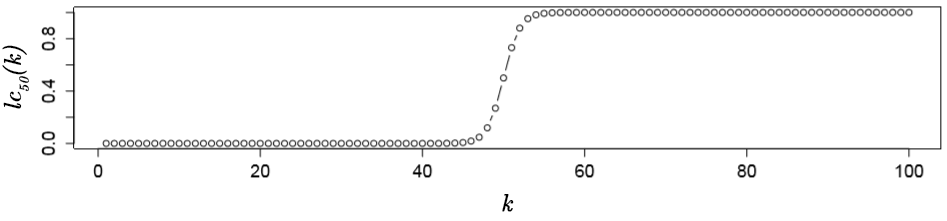
\includegraphics[width=\textwidth]{images/penalty-lc50}
    \caption{\emph{función de costo de latencia}, $lc_o(k)$, para $o=50$.}
\label{fig:lc50}
\end{figure}

De esta manera, la medida $ERDE_o$ acumulará error tanto cuando la clasificación sea incorrecta como cuando sea correcta pero habiéndose superado el umbral de decisión dado por $o$.
Por lo tanto, esta medida permite comparar el rendimiento de distintos modelos en relación a qué tan rápidos y efectivos sean ya que, mientras más rápido y más efectivo sea un modelo, más cercano a nulo será el error acumulado y, por lo tanto, más cercano a $0$ será su valor $ERDE_o$.\footnote{Como se verá en el \autoref{cap:eRisk2019}, esta medida no es perfecta, por ejemplo, si bien nos permitirá realizar comparaciones relativas entre modelos, su semántica en términos absolutos, sin contexto, no es tan clara (¿Qué significaría que el valor $ERDE_5$ obtenido sea de, por ejemplo, $11.31\%$?¿es el modelo rápido o lento?).
Por lo que, en dicho capítulo, se introducirá una medida adicional que buscará abordar algunos de estos aspectos.}
Además, el costo de una clasificación incorrecta no será igual cuando la decisión involucre a un usuario en riesgo que cuando no, ya que, en la práctica, se suele utilizar $c_{fn} \gg c_{fp}$ para reflejar el hecho de que cada usuario positivo no detectado (falso negativo) es una vida en riesgo y, en consecuencia, el costo a pagar en dicho caso es elevado ($c_{fn}$).\footnote{Además, esta elección ayuda a evitar la utilización de modelos triviales que clasifiquen a todos los usuarios como negativos.}

% Por ejemplo, si bien la medida $ERDE_o$ permite realizar comparaciones relativas entre modelos, su semántica en término de su valor absoluto no es tan clara.\footnote{¿Qué significa que el valor $ERDE_5$ obtenido haya sido de, por ejemplo, $11.31\%$?¿fue el modelo rápido o lento?}

%la medida $ERDE_o$ resaltará a los modelos que prioricen $recall$ por sobre $precision$,\footnote{Esto se debe a la forma en que se calcula la medida $ERDE_o$ (\autoref{eq:erde}), siendo el costo de los falsos positivos ($cfp$) considerablemente más pequeño que el de los falsos negativos ($cfn$).} lo que no es necesariamente malo teniendo en cuenta que se lidia con tareas de riesgo en donde cada usuario (positivo) no detectado es una vida en riesgo.

Finalmente, en la tarea piloto se utilizaron, específicamente, las medidas $ERDE_5$ y $ERDE_{50}$ y se fijaron los valores $c_{fn} = c_{tp} = 1$ y el valor $c_{fp}$ como el número de sujetos depresivos dividido por el total de sujetos en el conjunto de prueba, es decir, se fijó $c_{fp}= \frac{52}{401} = 0.129$.
%In order to avoid building trivial classifiers that always say no, we need to have $cfn >> cfp$





\subsection{Detalles de Implementación}
\label{sec:implementation}

El modelo propuesto fue codificado manualmente en \emph{Python 2.7} utilizando solamente funciones y estructuras de datos nativas, como ser \emph{dict} para los diccionarios o las funciones \emph{map} y \emph{reduce} para simular localmente el patrón \emph{MapReduce}.
Además, por simplicidad, se decidió utilizar la suma de vectores como implementación de los \emph{operadores de resumen}, $\oplus_j$, para todo nivel $j$.
Dado que este trabajo se centra en la detección anticipada, y no en aspectos vinculados al cómputo paralelo para clasificación a gran escala, no fue necesario realizar una implementación real del modelo de cómputo paralelo \emph{MapReduce}.
Además, implementar una versión \emph{MapReduce} no hubiera sido adecuada, ya que en la \autoref{subsec:exp-scenario2} analizamos el tiempo de cómputo de los clasificadores y todos ellos deben compartir el mismo tipo de implementación, sin paralelismo, para que la comparación sea justa.
Por el mismo motivo, todos los otros clasificadores utilizados en \autoref{subsec:exp-scenario2} fueron implementados con el paquete \emph{sklearn},\footnote{\url{https://scikit-learn.org/}} versión 0.17, también en \emph{Python 2.7}.
Además, para estos clasificadores se utilizó una representación de bolsa de palabras con pesado \emph{tf-idf}, por lo que la vectorización de la entrada se realizó con la clase \emph{TfidfVectorizer}. El preprocesamiento se llevó a cabo eliminando las palabras vacías\footnote{Utilizando la lista estándar de palabras vacías para el inglés.} y las palabras que tuvieran una frecuencia de documentos inferior a 20. Finalmente, estos clasificadores se implementaron utilizando sus correspondientes versiones ya integradas en \emph{sklearn}, tales como las clases \emph{LogisticRegression, KNeighborsClassifier}, o \emph{MultinomialNB}, entre otras.

% SS3 was manually coded in \emph{Python 2.7} using only built-in functions and data structures, e.g. a \emph{dict} to store the category's dictionary or \emph{map} and \emph{reduce} functions to (locally) simulate a \emph{MapReduce} pattern.
% Since this paper focuses on early detection, not computing nor large-scale classification, we did not perform a real \emph{MapReduce} implementation.
% Moreover, since in \autoref{subsec:exp-scenario2} we are also reporting the computation time taken by all the other classifiers and all of them must share the same type of implementation, implementing a \emph{MapReduce} version would not have been fair.
% Thus, all these other models were also implemented in \emph{Python 2.7}, using the \emph{sklearn} library\footnote{\href{https://scikit-learn.org/}{https://scikit-learn.org/}}, version 0.17. Vectorization was done with the \emph{TfidfVectorizer} class, with the standard English stop words list. Additionally, terms having a document frequency lower than 20 were ignored. Finally, classifiers were coded using their corresponding \emph{sklearn} built-in classes, e.g. \emph{LogisticRegression, KNeighborsClassifier, MultinomialNB}, etc.


\subsection{Experimentos y Resultados}
%\subsection{Comparison with Related work}
\label{sec:exp_and_results}

Esta subsección describe el trabajo experimental, el cual se llevó a cabo bajo dos escenarios diferentes.
En el primero, realizamos los experimentos de acuerdo con la definición original de la tarea piloto eRisk, utilizando los \emph{bloques} de publicaciones.
Sin embargo, dado que esta definición supone, mediante el uso de bloques, que el número total de publicaciones de cada usuario se conoce de antemano\footnote{Hecho que no se cumple en ambientes en  los que los usuarios generan contenido dinámicamente, tales como las redes sociales.}, decidimos considerar también un segundo tipo de experimento, uno que simule un escenario más realista en el que el historial de cada usuario sea procesado ``en flujo'', una publicación a la vez.
% This subsection describes the experimental work, which was divided into two different scenarios.
% In the first one, we performed experiments in accordance with the original eRisk pilot task definition, using the described \emph{chunks}.
% However, since this definition assumes, by using chunks, that the total number of user's writings is known in advance\footnote{Which is not true when working with a dynamic environment, such as Social Media.}, we decided to also consider a second type of experiment, simulating a more realistic scenario, in which user's history was processed in a streaming way, one writing (post) at a time.


\subsubsection{Escenario 1: clasificación incremental bloque a bloque (configuración original)} 

Como se tienen sólo dos clases con poco solapamiento entre ellas, decidimos fijar los hiperparámetros $\lambda$ y $\rho$ del modelo SS3 en $1$. De hecho, también realizamos algunas pruebas con otros valores que mejoraron la \emph{precision} o el \emph{recall} pero empeorando la medida \emph{ERDE}.
La optimización de hiperparámetros se realizó aplicando una \emph{búsqueda en grilla} sobre el hiperparámetro $\sigma$, minimizando la medida $ERDE_{50}$ sobre el conjunto de entrenamiento utilizando una \emph{validación cruzada de 4 iteraciones}. Además, la \emph{búsqueda en grilla} se llevó a cabo utilizando tres niveles diferentes de precisión. En el primer nivel, $\sigma$ tomó los valores $0.5\pm k\cdot10^{-1}$, con $k\in [0, 5]$. Una vez encontrado el mejor valor de $\sigma$, digamos $\widehat{\sigma_1}$, se comenzó una segunda búsqueda de ``segundo nivel'' en la que $\sigma$ tomó los valores $\widehat{\sigma_1}\pm k\cdot10^{-2}$. Finalmente, se realizó una tercer búsqueda al rededor de este nuevo mejor valor, $\widehat{\sigma_2}$, donde $\sigma$ tomó los valores $\widehat{\sigma_2}\pm k\cdot10^{-3}$, también con $k\in [0, 5]$.
% Since there were only two, barely overlapped, categories, we decided to start by fixing the SS3 framework's $\lambda$ and $\rho$ hyper-parameters to 1. In fact, we also carried out some tests with other values that improved the \emph{precision} (or \emph{recall}) but worsened the ERDE measure.
% Model selection was done by a 4-fold cross-validation on the training data minimizing the ERDE$_{50}$ measure while applying a \emph{grid search} on the $\sigma$ hyper-parameter. 
% This \emph{grid search} was carried out at three different levels of precision. In the first level, $\sigma$ took values from $0.5\pm k\cdot10^{-1}$, with $k\in [0, 5]$. Once the best value of $\sigma$ was found, let us say $\widehat{\sigma_1}$, we started a second level \emph{grid search} in which $\sigma$ took values from $\widehat{\sigma_1}\pm k\cdot10^{-2}$. Finally, a third search was applied around the new best value, $\widehat{\sigma_2}$, where $\sigma$ was set to $\widehat{\sigma_2}\pm k\cdot10^{-3}$, also with $k\in [0, 5]$. %, till the best value $\widehat{\sigma_3}$ was found.

\begin{table}[t]
\centering
\caption{Resultados para el escenario 1 (configuración original de la tarea piloto, lectura bloque a bloque).}
\label{tab:erisk-chunks}
\begin{tabular}{l@{}c || l@{}c}
\hline
& $ERDE_5\blacktriangle$ & & $ERDE_{50}\blacktriangle$\\ \hline
SS3 & \textbf{12.60\%} & SS3$^\Delta$ & \textbf{7.72\%}\\
SS3$^\Delta$ & 12.70\% & SS3 & 8.12\%\\
FHDO-BCSGB & 12.70\% & UNSLA & 9.68\%\\
UArizonaB & 13.07\% & FHDO-BCSGA & 9.69\%\\
UQAMD & 13.23\% & UArizonaD & 10.23\%\\
UNSLA & 13.66\% & UQAMD & 11.98\%\\
LyRE & 13.74\% & GPLC & 12.14\%\\
GPLC & 14.06\% & CHEPEA & 12.26\%\\
CHEPEA & 14.75\% & LyRE & 13.74\%\\
NLPISA & 15.59\% & NLPISA & 15.59\%\\ \hline

\hline
\end{tabular}
\end{table}

% \begin{table}[t]
% \centering
% \caption{Resultados para el escenario 1 (configuración original de la tarea piloto, lectura bloque a bloque).}
% \label{tab:erisk-chunks}
% \begin{tabular}{l@{}c || l@{}c}
% \hline
% & $ERDE_5\blacktriangle$ & & $ERDE_{50}\blacktriangle$\\ \hline
% \textbf{SS3}$\star$ & \textbf{12.70\%} & \textbf{SS3}$\star$ & \textbf{8.12}\%\\
% FHDO-BCSGB &\textbf{ 12.70\%} & UNSLA & 9.68\%\\
% UArizonaB & 13.07\% & FHDO-BCSGA & 9.69\%\\
% UQAMD & 13.23\% & UArizonaD & 10.23\%\\
% UNSLA & 13.66\% & UQAMD & 11.98\%\\
% LyRE & 13.74\% & GPLC & 12.14\%\\
% GPLC & 14.06\% & CHEPEA & 12.26\%\\
% CHEPEA & 14.75\% & LyRE & 13.74\%\\
% NLPISA & 15.59\% & NLPISA & 15.59\%\\ \hline

% \hline
% \end{tabular}
% \end{table}

Luego, usando la configuración de hiperparámetros que obtuvo el mejor valor para $ERDE_{50}$, $\lambda = \rho = 1$ y $\sigma = 0.455$, se entrenó el  modelo con el conjunto de entrenamiento completo y se realizó, finalmente, la clasificación de los sujetos en el conjunto de prueba.
Además, la clasificación del conjunto de prueba se llevó a cabo aplicando dos políticas de clasificación anticipada diferentes, de forma similar a lo que se introdujo intuitivamente en \autoref{sec:classification_process}:
la primer política clasifica a un sujeto como positivo cuando el \emph{valor de confianza} positivo acumulado supera al negativo;
la segunda política, utilizada por el modelo SS3$^\Delta$, es un poco más elaborada y clasifica a un sujeto como positivo cuando se cumple la primer política o cuando el valor de confianza positivo crece 4 veces más rápido que el negativo.\footnote{Se probaron valores distintos a 4, utilizando validación cruzada, pero fue este valor el que produjo el mejor resultado.}
% After the \emph{grid search}, using the hyper-parameter configuration with the lowest $ERDE_{50}$ value, $\lambda =\rho=1$ and $\sigma= 0.455$, we finally trained our model with the whole training set and performed the classification of the subjects from the test set.
% Additionally, the classification of the test set was carried out applying two different classification policies, similarly to what was intuitively introduced in \autoref{sec:classification_process}:
% the first one classified a subject as positive if the accumulated positive confidence value becomes greater than the negative one;
% the second one, denoted by SS3$^\Delta$, was more comprehensive and classified a subject as positive when the first case was met, or when the change of the positive slope was, at least, four times greater than the negative one, i.e. the positive value increased at least 4 times faster\footnote{Those readers interested in the implementation details for this scenario, the classification algorithm is given in the next section.}. 
Los resultados obtenidos se muestran en la \autoref{tab:erisk-chunks} y se comparan, entre los 30 modelos enviados, contra los mejores $ERDE_5$ y $ERDE_{50}$ de cada grupo de investigación.\footnote{Lista completa disponible en \href{http://early.irlab.org/2017/task.html}{early.irlab.org/2017/task.html}.}
Se puede observar que SS3 obtuvo el mejor $ERDE_5$ ($12.60\%$) mientras que SS3$^\Delta$ el mejor $ERDE_{50}$ ($7.72\%$).
Además, las medidas de desempeño tradicionales obtenidas fueron $F_1=0.52$, $presision=0.44$ y $recall=0.63$ para SS3 y $F_1=0.54$, $precision=0.44$ y $recall=0.69$ para SS3$^\Delta$. SS3$^\Delta$ tuvo el séptimo mejor valor de $F_1$ (0.54) entre las otras 30 contribuciones y fue bastante superior al promedio ($0.39$). Esto último no es del todo malo teniendo en cuenta que los hiperparámetros se seleccionaron con el objetivo de optimizar la medida $ERDE_{50}$, no $F_1$.
% The obtained results are shown in \autoref{tab:erisk-chunks} and are compared against each institution's best ERDE$_5$ and ERDE$_{50}$ among all the 30 submissions \footnote{The full list is available at \href{http://early.irlab.org/2017/task.html}{early.irlab.org/2017/task.html}.}.
% It can be seen that SS3 obtained the best ERDE$_5$ (12.60\%) while SS3$^\Delta$ the best ERDE$_{50}$ (7.72\%).
% Additionally, classical timeless measures were $F_1=0.52$, $\pi=0.44$ and $\rho=0.63$ for SS3 and $F_1=0.54$, $\pi=0.44$ and $\rho=0.69$ for SS3$^\Delta$. SS3$^\Delta$ had the 7th best $F_1$ value (0.54) out of the other 30 contributions and was quite above the average ($0.39$), which is not bad taking into account that hyper-parameters were selected with the aim of minimizing ERDE, not the $F_1$ measure.


\subsubsection{Escenario 2 - clasificación incremental publicación a publicación (configuración más realista)} \label{subsec:exp-scenario2} 


Como se mencionó anteriormente, en el escenario original, cada bloque contenía un $10\%$ del historial completo de publicaciones de cada sujeto. Sin embargo, dependiendo de qué tanto contenido haya creado cada sujeto, este $10\%$ podría significar sólo una única publicación para algunos sujetos, mientras que para otros, cientos o incluso miles de publicaciones. Además, el uso de bloques supone que conocemos con antelación la cantidad total de publicaciones de cada sujeto, lo que no es posible en la vida real, en donde los ambientes serán dinámicos y se crearán nuevas publicaciones con el paso del tiempo. Por lo tanto, decidimos realizar pruebas en un nuevo escenario más realista, sin el uso de bloques, en el que los sujetos son procesados ``en flujo''. Esto es, bajo este nuevo escenario, a los modelos se les entrega una publicación a la vez, simulando la creación de las mismas por parte de los sujetos ``en tiempo real''.
% As said earlier, each chunk contained 10\% of the subject's writing history, a value that for some subjects could be just a single writing while for others hundreds or even thousands of writings. Furthermore, the use of chunks assumes we know in advance all subject's writings, which is not the case in real life scenarios, in which writings are created over time. Therefore, in this new (more realistic) scenario, subjects were processed one writing at the time (in a stream-like way) and not using chunks. 

Dado que para este nuevo escenario no tenemos resultados previos disponibles de otros participantes, con el fin de comparar resultados, realizamos experimentos no sólo con SS3, sino también con los siguientes clasificadores tradicionales:\footnote{Los detalles de implementación de estos clasificadores se dieron en la \autoref{sec:implementation}.} \ac{SVM}, \ac{MNB}, \ac{RL} y \ac{k-NN}. Para todos estos clasificadores, como política de clasificación anticipada se utilizó la política que mostró mejores resultados en Losada \emph{et al.} \cite{losada2016test}: clasificar un sujeto como depresivo cuando la probabilidad del clasificador sea superior a $0.5$.
% Given that we do not have previous results available from other participants, under this new scenario, for comparison, we had to perform experiments not only with SS3 but also with other classical classifiers\footnote{Experiments with these classifiers were conducted using $scikit-learn$ Python library.} Logistic Regression (LOGREG), Support Vector Machine (SVM), Multinomial Naive Bayes (MNB) and $K$-Nearest Neighbors ($K$-NN). For all these standard methods, the policy to classify a stream as positive (depressed) was the same as the most effective policy used in \cite{losada2016test}, that is, classify a subject as depressed when the classifier outputs a confidence value above 0.5.

Como se discutirá en la siguiente sección, bajo este nuevo escenario en el que los sujetos se clasifican incrementalmente procesando ``un flujo de publicaciones'', el costo computacional de clasificador por cada sujeto es de orden cuadrático, $O(n^2)$, con respecto al número de publicaciones, $n$ ---excepto para los clasificadores \ac{MNB} y SS3 cuyo costo es lineal, $O(n)$.
De acuerdo con esto, realizar una validación cruzada, para encontrar los mejores parámetros de cada clasificador para minimizar la medida $ERDE$, tomaría un tiempo prohibitivo, ya que se demoraría más de una hora por cada combinación de valores de hiperparámetros y cada iteración de la validación cruzada posible.\footnote{Semanas o incluso meses dependiendo del clasificador.} Por lo tanto, los hiperparámetros de todos los cinco clasificadores se seleccionaron utilizando validación cruzada con el objetivo de optimizar la medida tradicional $F_1$, en lugar de la medida $ERDE$.
% As it will be discussed in the next section, when classifying a subject in a streaming-like way, the execution cost of each classifier for each subject is $O(n^2)$ with respect to the total number of subject's writings, $n$ ---except for MNB and SS3 which is $O(n)$.
% In accordance to this, if we had used cross-fold validation to find the best parameters of each classifier to minimize the ERDE measure it would have taken too much time, more than one hour for every single fold and for every single possible combination of parameter values (i.e. weeks or even months in total). Therefore, parameters were selected with the aim of optimizing, as usual, the standard F$_1$ measure instead of ERDE.

Dado que el conjunto de datos está altamente desbalanceado, se optimizó el parámetro de penalización, $C$ $(C> 0)$, y el parámetro de peso de clase, $w$ $(w\geq 1)$, para \ac{SVM} y \ac{RL}; para \ac{MNB} sólo se varió el peso de la clase $w$, mientras que para \ac{k-NN}, el parámetro $K$.
También, como en Losada \emph{et al.} \cite{losada2016test}, se estableció el peso de la clase mayoritaria, ``no depresivo'', en $1/(1 + w)$ y el peso de la clase minoritaria, ``depresivo'', en $w/(1 + w) $. Además, siguiendo prácticas tradicionales, se aplicó una \emph{búsqueda en grilla} sobre estos hiperparámetros con secuencias de crecimiento exponencial ($C = 2^{-10}, 2^{-4}, \cdots, 2^9$ y $w = 2^0, 2^1, \cdots, 2^9 $) para \ac{SVM}, \ac{RL} y \ac{MNB}; para el caso de \ac{k-NN}, $K$ tomó valores secuencialmente desde $1$ hasta $20$.
% Since the dataset was highly unbalanced we optimized the penalty parameter, $C$ $(C > 0)$, and the class weight parameter $w$  $(w \geq 1)$ for SVM and LOGREG; for MNB only the class weight $w$ was varied, while for $K$NN the $K$ parameter. 
% As in \cite{losada2016test}, we set the majority class (non-depressed) weight to $1/(1 + w)$ and the minority class (depressed) weight to $w/(1 + w)$. Also, following standard practice, we applied a grid search on the tuning parameters, with exponentially growing sequences ($C = 2^{-10}, 2^{-4}, \cdots, 2^9$ and $w = 2^0, 2^1, \cdots, 2^9$) for SVM, LOGREG, and MNB and for the case of $K$-NN, $K$ took values sequentially from 1 to 20.
Además, como en el escenario anterior, esta optimización se realizó usando una validación cruzada de 4 iteración sobre el conjunto de entrenamiento, optimizando en su lugar, como se mencionó, la medida $F_1$ con respecto a la clase minoritaria. La configuración de parámetros que obtuvo los mejores valores $F_1$ para cada clasificador fueron: $C = 16$ y $w = 16$ para \ac{SVM}, con regularización $L2$; $C = 16$ y $w = 4$ para \ac{RL}, con regularización $L1$; $w = 1$ para \ac{MNB}; $K = 2$ para \ac{k-NN}; y $\lambda = 1.68$, $\rho = 0.38$ y $\sigma = 0.5$ para SS3.
% Model selection was also done by 4-fold cross-validation on the training data optimizing the F$_1$ measure with respect to the minority class. The parameter configuration with the highest F$_1$ for each classifier were the following: $C=16$ and $w=16$ for SVM (with L2 regularization); $C=16$ and $w=4$ for LOGREG (with L1 regularization); $w=1$ for MNB; $K=2$ for KNN; and $\lambda= 1.68$, $\rho=0.38$ and $\sigma=0.5$ for SS3.

\begin{table*}[t!]
\centering
\caption{Resultados para el escenario 2 (configuración usando una variante más realista, lectura publicación a publicación).}
\label{tab:erisk-writings}
\centerline{
\begin{tabular}[c]{l c c c c c c c c c c}
\hline
& \multicolumn{6}{c}{$ERDE_o$} & $F_1$ & $precision$ & $recall$ & tiempo \\
& $o = 5$ & $o = 10$ & $o = 30$ & $o = 50$ & $o = 75$ & $o = 100$  & & & & \\ \hline

RL & 11.7\% & 10.9\% & 9.4\% & 7.5\% & 6.3\% & 5.8\% & 0.53 & 0.41 & 0.75  & 1h + 11.3m \\
SVM & 12.0\% & 10.9\% & 9.1\% & \textbf{7.2}\% & 6.1\% & 6.0\% & \textbf{0.55} & \textbf{0.47} & 0.69 & 1h + 13.9m \\
MNB & \textbf{10.6\%} & 10.4\% & 10.4\% & 10.4\% & 10.1\% & 10.1\% & 0.24 & 0.14 & \textbf{1} & 17.5m \\
KNN & 12.6\% & 10.4\% & 8.5\% & 8.2\% & 7.9\% & 7.7\% & 0.35 & 0.22 & 0.90 & 1h + 40.6m \\
SS3 & 11.0\% & \textbf{9.8\%} & \textbf{8.0\%} & \textbf{7.2\%} & \textbf{5.8\%} & \textbf{5.5\%} & 0.54 & 0.42 & 0.77 & \textbf{3.7m} \\
SS3$^\Delta$ & 11.1\% & 9.9\% & 8.1\% & 7.3\% & 5.9\% & 5.6\% & \textbf{0.55} & 0.42 & 0.81 & \textbf{3.7m} \\ \hline

\hline
\end{tabular}
}
\end{table*}

Luego, utilizando esta mejor configuración de hiperparámetros, los clasificadores fueron entrenados con el conjunto de entrenamiento completo y, finalmente, se procedió a realizar la clasificación incremental de cada sujeto de prueba, una publicación a la vez. Además, se decidió calcular la medida $ERDE$ no sólo para $o = 5$ y $50$, sino también para $o = 10$, $30$, $75$, y $100$ con el fin de tener una visión más amplia de cuán eficientes son los clasificadores con respecto a qué tan temprano deciden clasificar. Los resultados obtenidos se muestran en la \autoref{tab:erisk-writings}.
En esta tabla se decidió incluir en la última columna, a modo de guía, el tiempo de cómputo que cada clasificador requirió para clasificar a todos los sujetos. Como podemos ver, SS3 obtuvo los mejores valores $F_1$ y $ERDE_o$ para todos los valores $o$ considerados, excepto para $ERDE_5$.
Por otro lado, SS3 obtuvo el segundo mejor valor para \emph{precision} (0.42), con un valor relativamente cercano al mejor (0.47), obtenido por \ac{SVM}.
Sin embargo, el tiempo de cómputo de SS3, dada su naturaleza incremental, es más eficiente en comparación a los otros modelos ---salvo \ac{MNB} que también puede trabajar incrementalmente. Por ejemplo, \ac{SVM} tardó más de una hora (1 hora y 13.9 minutos) en completar la clasificación del conjunto de prueba, mientras que a SS3 le tomó una pequeña fracción de ese tiempo llevar a cabo la misma tarea ---3.7 minutos, sólo un $5\%$ del tiempo que le tomó a \ac{SVM}.
% We trained the classifiers using the optimized parameters with the whole training dataset and then, the incremental post-by-post classification was analyzed. Now, writings are processed sequentially, that is, early classification evaluation was carried out, as mentioned, one writing (post) at a time. Additionally, we decided to compute the ERDE measure not only for $o=5$ and 50 but also for $o=10$, 30, 75 and 100 in order to have a wider view of how efficient classifiers are with respect to how early they classify subjects. The obtained results are shown in \autoref{tab:erisk-writings}.
% There, in the last column, it is also included the time that each classifier required to classify all the subjects in the test set. As we can see, SS3 obtained the best $F_1$ and ERDE values for all the considered $o$ values except for ERDE$_5$.
% On the other hand, SS3 has a precision($\pi$) value (0.42) relatively similar to the best one (0.47), obtained by SVM.
% However, as we will discuss further in the next section, SS3 has a more efficient computation time in comparison with the remaining algorithms. For instance, it took SVM more than one hour (73.9 minutes) to complete the classification of the test set while it took SS3 a small fraction of it (roughly 5.3\%) to carry out the same task

\begin{table}[t!]
\centering
\caption{Resultados para la clasificación tradicional, no anticipada. Cada sujeto se representa como un único documento formado por todas sus publicaciones.}
% \caption{Results on the test set using all subject's history as a single document, i.e. timeless classification.}
\label{tab:erisk-fulldoc}
\begin{tabular}{l c c c}
\hline
& $F_1$ & $precision$ & $recall$ \\ \hline
SS3 & \textbf{0.61} & \textbf{0.63} & 0.60 \\
LOGREG & 0.59 & 0.56 & 0.63  \\
SVM & 0.55 & 0.5 & 0.62 \\
MNB & 0.39 & 0.25 & \textbf{0.96} \\
KNN & 0.54 & 0.5 & 0.58 \\ \hline

\hline
\end{tabular}
\end{table}

Finalmente, es interesante mencionar que, además, realizamos la clasificación de los sujetos de manera tradicional, no anticipada, es decir, se utilizaron todas las publicaciones de cada sujeto como si fueran un único gran documento; los resultados obtenidos se muestran en la \autoref{tab:erisk-fulldoc}.
Como se puede observar, SS3 obtuvo los valores más altos para las medidas $F_1$ ($0.61$) y \emph{precision} ($0.63$), tal vez, debido a la flexibilidad que sus tres hiperparámetros brindan a la hora de descubrir términos importantes y discriminativos. Estos resultados sugieren que SS3 también puede lograr un desempeño competitivo cuando se lo entrena para optimizar medidas de evaluación tradicionales, como fue en este caso $F_1$.
Notar que la mejor configuración obtenida de \ac{MNB}, luego de la etapa de optimización de hiperparámetros, al parecer tiende a clasificar a la mayoría de los sujetos como depresivos, es por esto que obtuvo un \emph{recall} cercano a $1$ pero una \emph{precision} muy baja ($0.25$) ---tal vez como producto de intentar solucionar el problema del desbalance de clases.
% It is interesting to notice that we also performed classification of subjects on the test set using all subject's writings as if it were a single document (i.e. classical timeless classification); results are shown in \autoref{tab:erisk-fulldoc}.
% SS3 obtained the highest values for $F_1$ (0.61) and Precision (0.63) measures, possibly due to the flexibility that is given by its three hyper-parameters to discover important and discriminative terms. These results provide strong evidence that SS3 also achieves competitive performance when is trained and tested to optimize classical (non-temporal) evaluation measures.  
% Note that the best configuration of MNB obtained after the model selection stage, aiming at overcoming the unbalanced dataset problem, tends to classify all subjects as depressed, that is the reason MNB had a Recall($\rho$) close to 1 but a really poor precision (0.25).


\section{Análisis y Discusión}
\label{sec:analysisAndDiscussion}

En base al estudio experimental detallado anteriormente, podemos concluir que el nuevo modelo propuesto, SS3, parece mostrar un desempeño notable frente a la tarea piloto de detección temprana de depresión, en relación a los otros modelos utilizados. Obtuvo los mejores resultados en relación a la medida $ERDE$, específicamente diseñada para combinar la efectividad y la demora de la clasificación. En este contexto, es importante resaltar que SS3 mostró ser más efectivo a pesar de ser, esencialmente, más simple que otros modelos más elaborados participando en esta tarea, como los modelos basados en grafos, los basados en ensamble de múltiples clasificadores o los basados en Redes Neuronales Recurrentes, tales como las \emph{LSTM} o las \emph{GRU}.
% como aquellos basados en Redes Neuronales Recurrentes, como las \emph{LSTMs} y \emph{GRUs}, modelos basados en gráfos o ensamble de múltiples clasificadores.
% From the experimental study of \autoref{sec:exp_and_results} we can conclude that the proposed framework, SS3, appears to show remarkable performance in incremental classification for early depression detection tasks. It obtained the best results for the time-aware error measures specifically designed to combine classifier’s accuracy and penalization in late classifications. In that context, it is important to notice that SS3 showed to be more effective than the others, very elaborated, approaches participating in the eRisk task, such as those based on Recurrent Neural Networks (like LSTM, GRU, etc.), graph-based models, ensembles of different classifiers, etc.

Además, como se intuyó en base a los resultados obtenidos en el segundo escenario de experimentación, SS3 es un método eficiente en términos de tiempo de cómputo.
Esto se debe al hecho de que, como vimos, SS3 fue diseñado para trabajar incrementalmente, por lo que, a diferencia de la gran mayoría de clasificadores, no necesariamente ve la entrada como un vector m-dimensional que debe calcularse antes de hacer una predicción. En consecuencia, como se observó en la \autoref{tab:erisk-writings}, al tener que recomputar continuamente sus vectores desde cero,\footnote{Aquí asumiremos que la representación utilizada no puede calcularse incrementalmente. Para el caso de representaciones que sí puedan actualizarse incrementalmente, no será necesario recomputar el vector desde cero, pero se tendrá que pagar el costo de almacenar y mantener toda la información necesaria para realizar dicha actualización. Sin embargo, independientemente del caso, este tipo de modelos siempre toma como entrada la (representación de la) secuencia \emph{completa} leída hasta el momento.} la demora en tiempo de ejecución de los clasificadores \ac{SVM}, \ac{RL} y \ac{k-NN} fue en un orden de magnitud superior ---\emph{i.e.} no en términos de minutos sino de horas. %cuando se trabaja con un flujo de texto, por ejemplo,  tienen recomputar dicho vector desde cero cada vez que se agrega nuevo contenido al flujo de entrada.
% Furthermore, as it was briefly shown in the experimental study, SS3 is also an efficient (in computation time) method.
% This is due to the fact that, unlike most state-of-the-art classifiers, SS3 does not necessarily see the input as an atomic m-dimensional vector (i.e. a document vector) that must be computed entirely before making a prediction. In consequence, when working with a sequence of documents, for instance, SVM, LOGREG, and KNN must re-compute the input vector each time new content is added to a sequence that needs to be classified.
Siendo más precisos, formalmente tenemos que si $n$ es la longitud de la secuencia de entrada, en este caso el número de publicaciones, cuando se trabaja con clasificadores capaces de procesar naturalmente secuencias como SS3, MNB o Redes Neuronales Recurrentes, el costo del algoritmo de clasificación anticipada, por cada sujeto, será igual a $n$ ---ya que cada publicación debe ser procesada una única vez.\footnote{En contexto de streaming, a este tipo de algoritmos se los denomina como \emph{one-pass algorithms}.}
Por otro lado, para clasificadores como \ac{SVM}, \ac{RL}, \ac{k-NN} o Redes Neuronales tradicionales (no recurrentes), este costo será igual a $n\times(n + 1)/2 = 1+2+... +n$ ---dado que la primer publicación debe procesarse $n$ veces, la segunda $n-1$, la tercera $n-2$, y así.
Por lo tanto, usando la \emph{Notación O Grande}, tenemos que los clasificadores incrementales pertenecen a $O(n)$, mientras que los otros pertenecen a $O(n^2)$.
% Finalmente, vale la pena mencionar que, como se señaló en la sección anterior, este costo no sólo afecta la etapa de clasificación en sí sino que también afecta severamente las etapas previas, como por ejemplo la optimización de hiperparámetros, ya que el conjunto de validación necesitará clasificarse múltiples veces durante la búsqueda, pagando dicho costo en cada iteración.
% Formally, if $n$ is the length of the sequence, when working with classifiers like SS3 or MNB, the cost of the early classification algorithm for every subject, according to the number of processed documents, is equal to $n$ (since each document needs to be processed only once). On the other hand, for classifiers like SVM, LOGREG, KNN or traditional Neural Networks, this cost is equal to $n\times(n+1)/2 = 1+2+...+n$ (since the first document needs to be processed $n$ times, the second $n-1$, the third $n-2$, and so on). Therefore, using the \emph{Big O Notation}, we have MNB and SS3 belonging to $O(n)$ whereas the other three classifiers belong to $O(n^2)$. Finally, it is worth mentioning that, as pointed out in the previous section, this cost affects not only the classification stage but it also severally affects previous stages such as hyper-parameter and model optimization since they usually need to classify the validation set several times (paying the cost every time).
Finalmente, vale la pena señalar aquí que la diferencia en términos de espacio también es significativa. Para los clasificadores que admiten clasificación incremental, sólo es necesario almacenar un pequeño vector para cada usuario. Por ejemplo, cuando usamos SS3 sólo necesitamos almacenar el \emph{vector de confianza}\footnote{En el caso de detección de depresión, un simple vector de dos dimensiones.} de cada usuario ---el cual simplemente se actualizaría poco a poco procesando el nuevo contenido que se genere.
Sin embargo, cuando se trabaja con clasificadores convencionales, por cada usuario necesitamos almacenar o bien todas sus publicaciones para construir la matriz documento-término o la matriz ya calculada, para actualizarla a medida que se genere nuevo contenido.
Notar que el almacenamiento de todas las publicaciones o una matriz documento-término de $d\times t$, donde $d$ es la cantidad de publicaciones y $t$ el tamaño del vocabulario, no se compara con el almacenamiento de un simple vector.
% It is worth noting that the difference in terms of space complexity is also very significant. For classifiers supporting incremental classification, like SS3 or MNB, only a small vector needs to be stored for each user. For instance, when using SS3 we only need to store the \emph{confidence vector}\footnote{In case of ADD, a 2-dimensional vector.} of every user and then simply update it as more content is created. However, when working with classifiers not supporting incremental classification, for every user we need to store either all her/his writings to build the document-term matrix or the already computed document-term matrix to update it as new content is added. Note that storing either all the documents or a $d\times t$ document-term matrix, where $d$ is the number of documents and $d$ the vocabulary size, takes up much more space than a small 2-dimensional vector.
De hecho, dado que las plataformas en línea, como las redes sociales, tienen cientos de miles o millones de usuarios, pagar un costo cuadrático para procesar cada uno de los usuarios, sumado a tener que almacenar una enorme matriz de $d\times t$ para cada uno de ellos, vuelven a los clasificadores que no admiten clasificación incremental no escalables e impracticables.
% Finally, since online social media platforms typically have thousands or millions of users, paying a quadratic cost to process each one while having to store either all the writings or a large $d\times t$ matrix for every user makes classifiers not supporting incremental classification not scalable.


Con respecto a la política de clasificación anticipada utilizada por SS3, podríamos decir que, aunque las reglas que se utilizaron fueron muy simples, mostraron ser más efectivas que otras políticas más elaboradas y complejas utilizadas en esta tarea por otros enfoques.
Por ejemplo, algunas de estas políticas incluían mecanismos de decisión complejos basados en reglas específicas para cada bloque de publicaciones diferente\cite{errecaldetemporal}, otras tenían en cuenta las decisiones de diferentes clasificadores, listas personalizadas con palabras específicas obtenidas con ganancia de información, hacían uso de fuentes externas de información o basaban su política en reglas hechas a mano, específicamente diseñadas para esta tarea en particular \cite{trotzek2017linguistic}, de la forma: ``si la salida $\geq\alpha_n$ y el número de publicaciones $\geq n$, entonces clasificar como positivo'', ``si la salida $\leq\beta_n$ y el número de publicaciones $\geq n$, entonces clasificar como no depresivo'', entre otras.
% Regarding the support that SS3 provides for early classification we can say that, even though the rules we used are very simple, they are more effective than very elaborated and complex mechanisms used in the pilot task. For instance, some mechanisms to stop reading and classifying a subject included complex decision mechanisms based on specific rules for the different chunks \cite{errecaldetemporal}. These rules take into account the decisions of different classifiers, the probability that each classifier assigned to its prediction, ``white lists'' containing the words with the highest information gain, and other sources of information.  Another approach that showed a good performance relied on hand-crafted rules specifically designed for this problem \cite{trotzek2017linguistic}, of the form: ``if output $\geq\alpha_n$ and number of writings $\geq n$, then classify as positive'', ``if output $\leq\beta_n$ and the number of writings $\geq n$, then classify as non-depressed'', etc.
Además, es interesante notar que si bien las dos políticas sencillas que utilizamos con SS3 son independientes del problema abordado\footnote{Ya que no utilizan ningún tipo de información específica vinculada, en algún aspecto, al problema abordado.}, obtuvieron mejores resultados en la práctica.
Quizás podríamos haber utilizado métodos más elaborados para aprender en simultáneo el modelo de clasificación y la política, como en otros trabajos encontrados en la literatura~\cite{dulac2011text, yu2017learning}.
Sin embargo, como las dos políticas simples fueron lo suficientemente efectivas como para superar a la de los otros métodos, decidimos dejar para trabajo a futuro el estudio del uso de políticas más elaboradas y centrarnos aquí sólo en el potencial del modelo en sí.
% As we can see, the two types of decision rules for early classification we used are quite simpler than those mechanisms and more importantly, they are problem-independent yet, interestingly, obtained better results in practice.
% It is true that more elaborated methods that simultaneously learn the classification model and the policy to stop reading could have been used, such as in \cite{dulac2011text,yu2017learning}.
% However, for the moment it is clear that this very simple approach is effective enough to outperform the remainder methods, leaving for future work the use of more elaborated approaches.

\

\begin{figure}[t!]
%    \begin{subfigure}{0.5\textwidth}
%        \centering
%        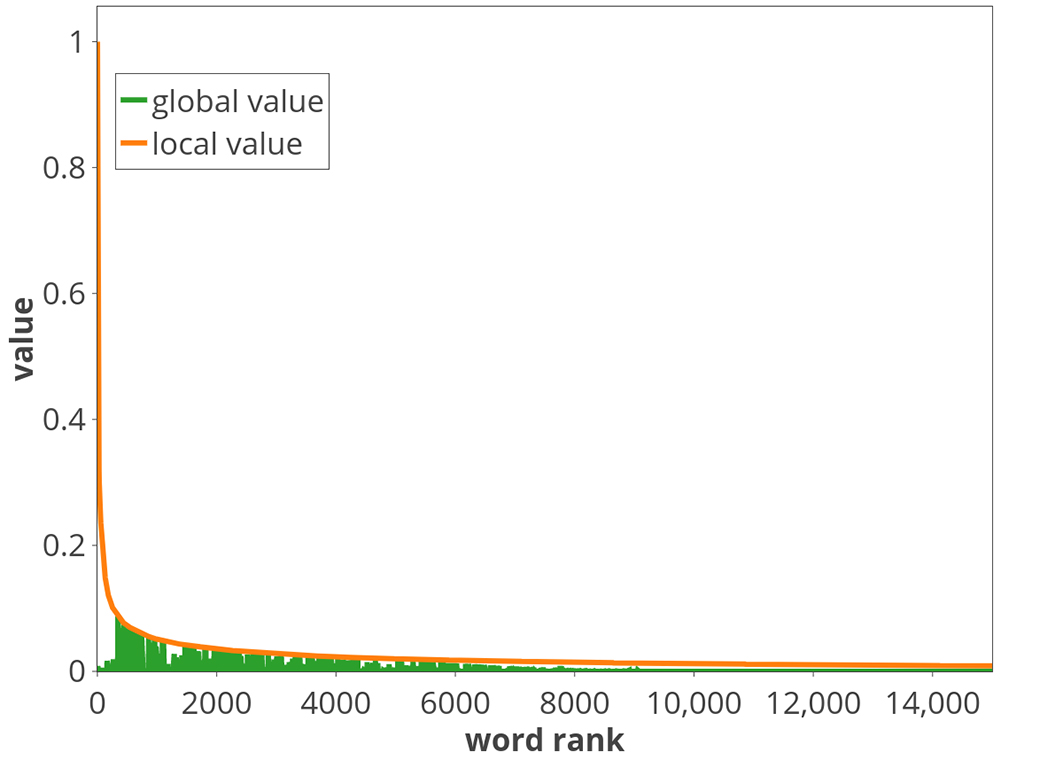
\includegraphics[width=90mm]{images/gv_negative}
%        \caption{Non-depressed}
%        \label{fig:gv_a}
%    \end{subfigure}
    % \begin{subfigure}{0.5\textwidth}
        \centering
        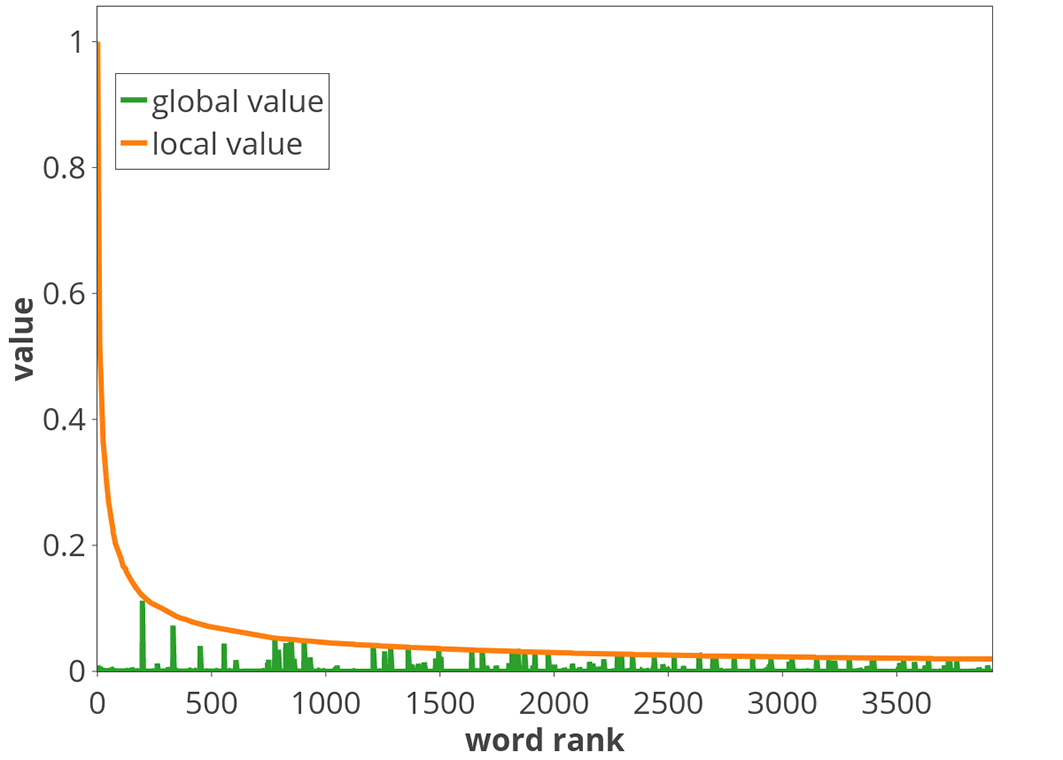
\includegraphics[width=90mm]{images/gv_positive}
        %\caption{Depressed}
        %\label{fig:gv_b}
    % \end{subfigure}
\caption{
    Curva con la distribución del \emph{valor local} de las palabras (en naranja) en contraste con la distribución del \emph{valor global} (en verde), obtenidas tras la experimentación para la clase ``depresivo''. La abscisa representa el ranking de las palabras individuales ordenadas por \emph{valor local}.
    Notar que la zona en la que se ubicarían las \emph{palabras vacías} (al comienzo de la abscisa, cercano al $0$) los \emph{valores locales} para esas palabras son los más altos (ya que el valor local de una palabra es proporcional a su frecuencia), sin embargo, como se esperaba, sus \emph{valores globales} son prácticamente $0$.
    % \emph{global value} (green) in relation to the \emph{local value} (orange) for the ``depressed'' category. The abscissa represents individual words arranged in order of frequency.
    % Note that the zone in which stop words are located (close to 0 in the abscissa) the  \emph{local value} is very high (since they are highly frequent words) but the \emph{global value} is almost 0, which is the desired behavior.
}
\label{fig:gv}
\end{figure}

\begin{figure*}[t!]
    \begin{subfigure}{0.5\textwidth}
        \centering
        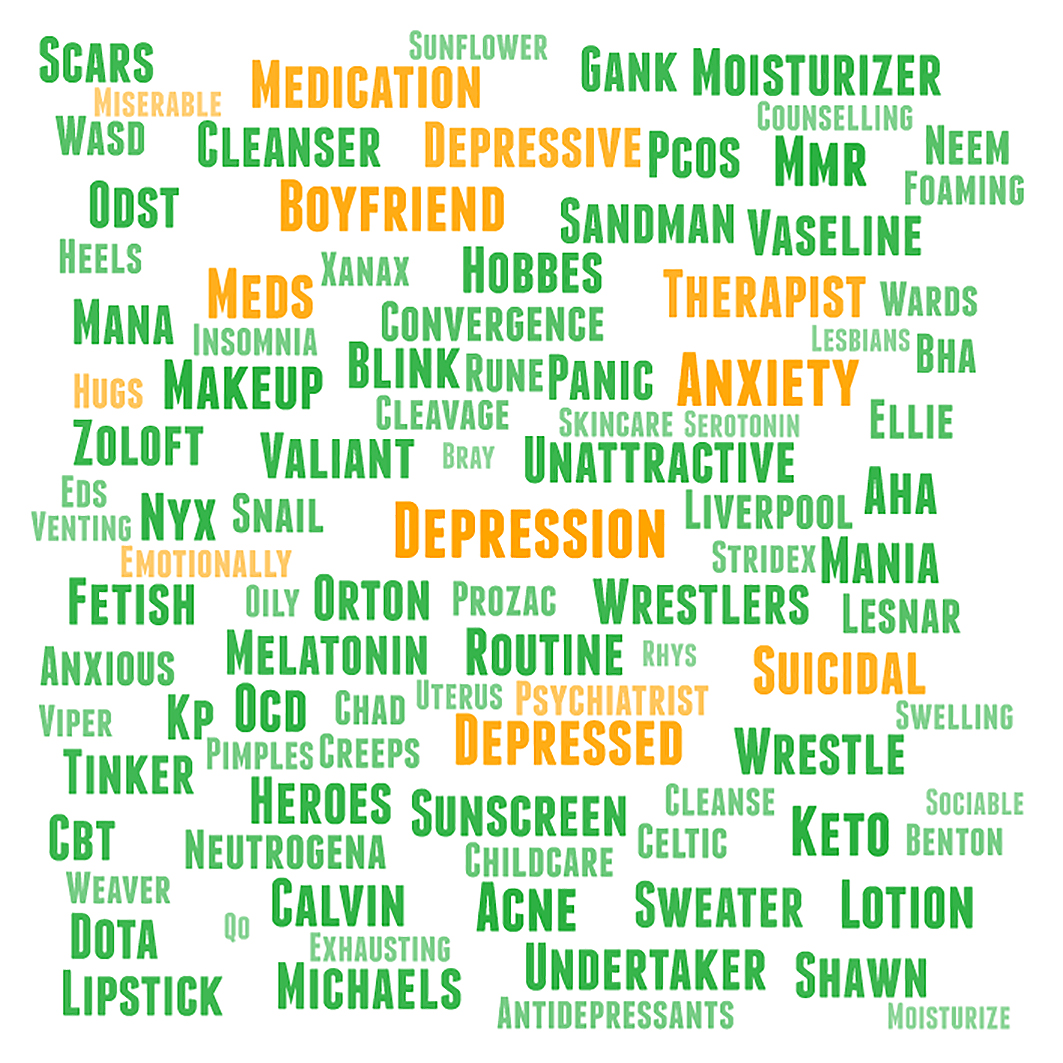
\includegraphics[width=\textwidth]{images/word-cloud-gv}
        \caption{Tamaño por \emph{valor global}}
        \label{fig:word_cloud_a}
    \end{subfigure}
    \begin{subfigure}{0.5\textwidth}
        \centering
        
\includegraphics[width=\textwidth]{images/word-cloud-gv-fr}
        \caption{Tamaño por frecuencia en bruto}
        \label{fig:word_cloud_b}
    \end{subfigure}
\caption{
    Top 100 palabras seleccionadas por \emph{valor global} obtenidas desde el modelo, tras la experimentación.
    El tamaño de las palabras representa (a) el \emph{valor global} y (b) la frecuencia en bruto.
    Además, con fines de comparación, en naranja se marcan aquellas palabras que también fueron seleccionadas entre las 100 primeras por \emph{ganancia de información}.
    % Top-100 words selected by \emph{global value (GV)} from the model trained for the eRisk Pilot Task using chunks. The font size is related to (a) \emph{GV} and (b) row frequency. The green color indicates the words selected only by \emph{GV} whereas the orange color indicates the words also selected by the traditional Information Gain(\emph{IG}).
}
\label{fig:word_cloud}
\end{figure*}

Con el fin de intentar comprender mejor las razones que puedan estar detrás del buen desempeño del modelo en la tarea abordada, consideramos importante comenzar por analizar los valores que aprendió a asignarle a cada palabra.
En la \autoref{fig:gv} se puede corroborar que empíricamente, como esperábamos, los \emph{valores globales} en la zona en la que se deberían encontrar las palabras más importantes y discriminatorias según la ley de Zipf\footnote{Como se hipotetizó por primera vez en \cite{luhn1958automatic}, esta ley empírica sostiene que las palabras de frecuencia media en la distribución, tienen mayor importancia y poder discriminativo que las palabras con alta frecuencia.}, efectivamente, fueron los más altos. 
% In order to get a better understanding of the rationale behind the good behavior of our framework, it is important to go into more details on the mechanisms used to weight words.
% In \autoref{fig:gv} we can empirically corroborate that the \emph{global value} correctly captures the significance and discriminating power of words since, as it is well known, mid-frequency words in the distribution have both high significance and high discriminating power\footnote{As firstly hypothesized by \cite{luhn1958automatic}.}, and \emph{global values} for these mid-frequency words are the highest.
Además, la valoración aprendida de las palabras puede apreciarse desde un punto de vista más cualitativo en las nubes de palabras mostradas en la  \autoref{fig:word_cloud}. % con las 100 palabras seleccionadas por mayor \emph{valor global}.
A partir de esta figura, es posible observar que, a diferencia de la tradicional \emph{ganancia de información} que sólo consideró palabras con alta frecuencia entre sus 100 primeras (ver tamaño de palabras en naranja en (b)), el \emph{valor global} consideró además palabras que, si bien no son tan frecuentes, sí son muy discriminativas.
Para resaltar este punto, notar que el \emph{valor global} consideró palabras muy generales (como ``depression'', ``suicidal'', ``psychiatrist'', ``anxiety'', entre otras), pero, a diferencia de \emph{ganancia de información}, también incluyó muchas palabras específicas.
Por ejemplo, por medio del \emph{valor global}, SS3 no sólo aprendió a reconocer la palabra antidepresivo (``antidepressant''), sino también antidepresivos específicos como \emph{Prozac} y \emph{Zoloft}\footnote{No se incluye aquí, pero también en la posición 125 se encontraba \emph{Lexapro}.};
no sólo términos generales relacionados con medicina o trastornos (como ``medication'', ``meds'', ``insomnia'', ``panic'' o ``mania''), sino también términos más específicos como \emph{OCD} (Trastorno Obsesivo Compulsivo), \emph{PCOS} (Síndrome de Ovario Poliquístico), \emph {EDS} (Síndrome de Ehlers-Danlos), \emph{CBT} (Terapia Cognitiva Conductual), \emph{serotonina}, \emph{melatonina}, \emph{Xanax} o \emph{KP} (Kaiser Permanente, una compañía de salud);
no sólo palabras generales relacionadas con dieta, el cuerpo o la apariencia (como ``unattractive'', ``skincare'', ``makeup'' o ``acne''), sino también \emph{pimples} (granos o espinillas faciales), \emph{swelling} (hinchazón), \emph{Keto} (dieta Keto o cetogénica para la depresión), \emph{Stridex} (una medicina de tratamiento y prevención del acné), \emph{AHA} (alfa hidroxiácidos), \emph{BHA} (beta hidroxiácido), \emph{Moisturizer} (humectante), \emph{NYX} (una compañía de cosméticos) o \emph{Neutrogena} (una marca de cosméticos para el cuidado de la piel y el cabello).
Vale la pena mencionar que éste no es un aspecto menor: si valoráramos a estos términos específicos solamente por su frecuencia/probabilidad\footnote{Como es el caso, por ejemplo, al usar el clasificador \ac{MNB}.}, siempre tendrán muy poco valor, ya que, naturalmente, la probabilidad de ocurrencia de estas palabras específicas es baja en comparación con palabras más generales, como se puede observar en (b). No obstante, nosotros como humanos sabríamos intuitivamente que, por ejemplo, las oraciones ``estoy tomando antidepresivos''  y ``estoy tomando Prozac'' tienen prácticamente el mismo valor en relación a decidir si el sujeto en cuestión es depresivo o no. Afortunadamente, este aspecto es capturado correctamente por el \emph{valor global}\footnote{Notar que, a diferencia de en (b), el tamaño de ``antidepressants'' y ``prozac'', respectivamente en la parte inferior y en el centro de (a), son bastante similares y no demasiado distintas a ``depression''.}, ya que efectivamente se formuló con el fin de valorar a los términos, globalmente, en relación a qué tan discriminatorias y relevantes son para cada clase.
% 	This discriminating power of words can also be appreciated from a more qualitative point of view in the word-clouds of the top-100 selected words by \emph{global value} shown in \autoref{fig:word_cloud}.
% 	From this figure it is possible to observe that the most frequent terms, i.e. the biggest ones on (b), were also selected by $IG$ (orange colored), however, most of the terms selected only by $GV$ (green colored) are not so frequent, but highly discriminative.
% 	To highlight this point, note that \emph{GV} included very general words (depression, suicidal, psychiatrist, anxiety, etc.) but, unlike \emph{IG}, it also included many specific words.
% For instance: not only the word \emph{antidepressant} was included but also well-known antidepressants such as \emph{Prozac} and \emph{Zoloft}\footnote{Not included here, but also at rank 125 \emph{Lexapro}.};
% not only general terms related to medicine or disorders (such as \emph{medication, meds, insomnia, panic, mania}, etc.) but also more specific ones such as \emph{OCD}(Obsessive compulsive disorder), \emph{PCOS}(Polycystic ovary syndrome), \emph{EDS}(Ehlers-Danlos syndrome), \emph{CBT}(Cognitive behavioral therapy), \emph{serotonin}, \emph{melatonin}, \emph{Xanax}, \emph{KP}(Kaiser Permanente, a healthcare company), etc.;
% not only general words linked to diet, body or appearance (such as \emph{unattractive, skincare, makeup, acne}, etc.) but also \emph{pimples}, \emph{swelling}, \emph{Keto} (Ketogenic diet for depression), \emph{Stridex} (an American acne treatment and prevention medicine), \emph{AHA}(Alpha hydroxy acids), \emph{BHA}(Beta hydroxy acid), \emph{Moisturizer}, \emph{NYX} (a cosmetics company), \emph{Neutrogena} (an American brand of skin care, hair care and cosmetics), etc.
% It is also worth mentioning that this is a vital and very relevant aspect: if we value these specific words, as is usual, only by their local probability \footnote{Which is the case, for instance, with Multinomial Naive Bayes.} (or frequency), as shown in (b), they will always have almost ``no value'' since, naturally, their probability of occurrence is extremely small compared to more general words (and even worst against stopword-like terms). However, for instance, we intuitively know the phrase ``I'm taking antidepressants'' has almost the same value as ``I'm taking Prozac'' when it comes to deciding whether the subject is depressed or not.
% Fortunately, this is correctly captured by the \emph{global value}\footnote{Note that, unlike in (b), the size of ``Antidepressants'' and ``Prozac'' in (a), at the bottom and in the middle of it respectively, are quite similar and not so different from the size of ``Depression''.} since it was created to value terms, globally, according to how discriminative and relevant they are to each category.

\

\begin{figure*}[t!]
    \begin{subfigure}{0.5\textwidth}
        \centering
        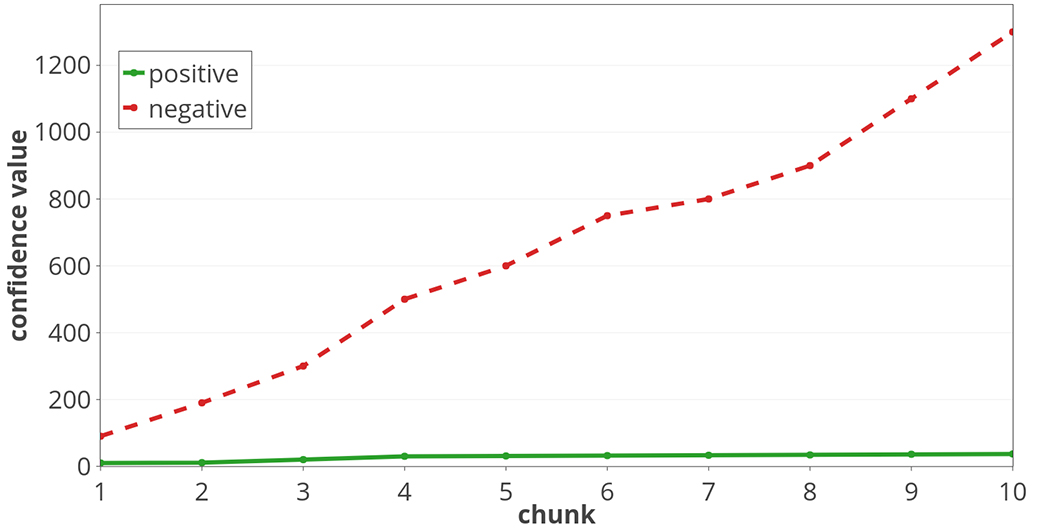
\includegraphics[width=\textwidth]{images/test_subject265}
        \caption{Sujeto 265, no depresivo.}
        \label{fig:subjects_gv_a}
    \end{subfigure}
    \begin{subfigure}{0.5\textwidth}
        \centering
        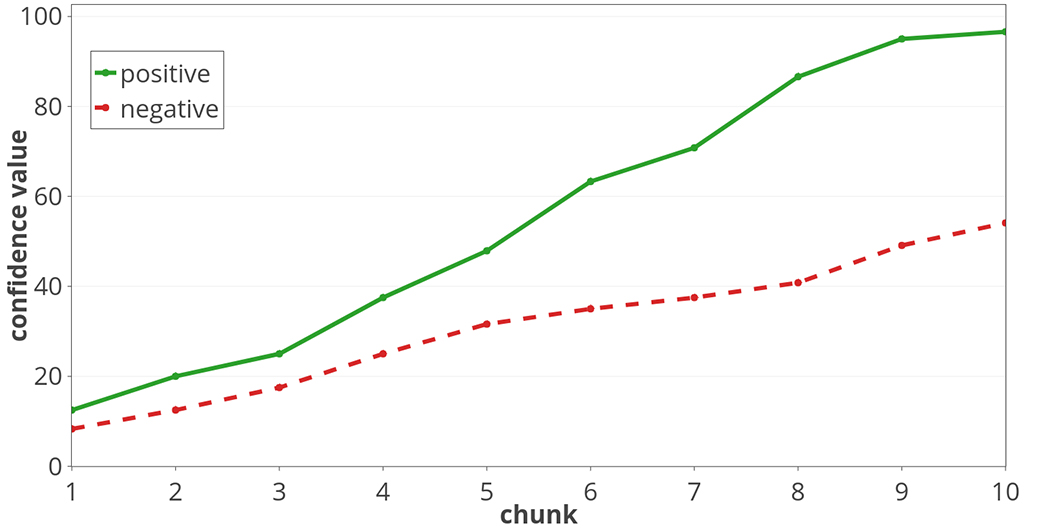
\includegraphics[width=\textwidth]{images/test_subject9306}
        \caption{Sujeto 9306, depresivo.}
        \label{fig:subjects_gv_b}
    \end{subfigure} \\
    \begin{subfigure}{0.5\textwidth}
        \centering
        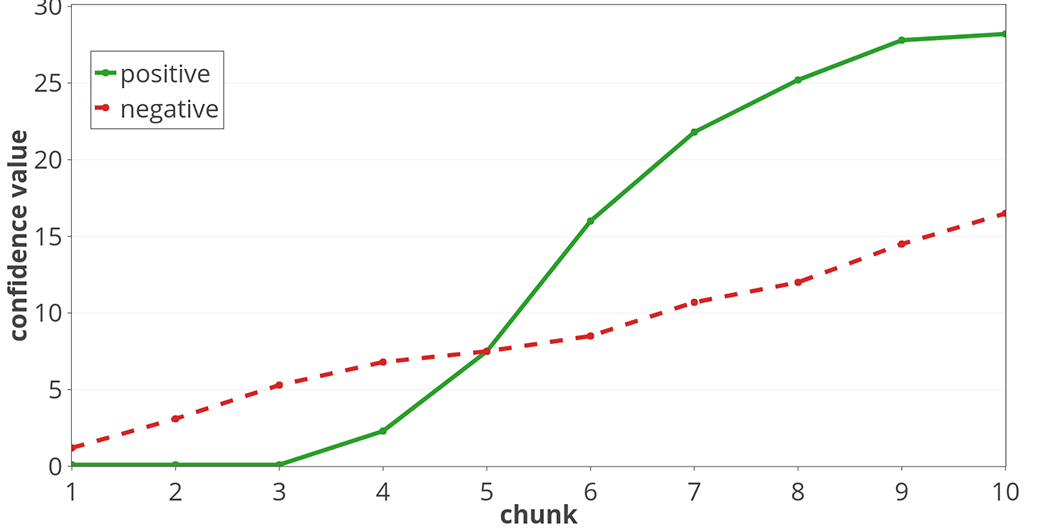
\includegraphics[width=\textwidth]{images/test_subject9579}
        \caption{Sujeto 9579, depresivo.}
        \label{fig:subjects_gv_c}
    \end{subfigure}
    \begin{subfigure}{0.5\textwidth}
        \centering
        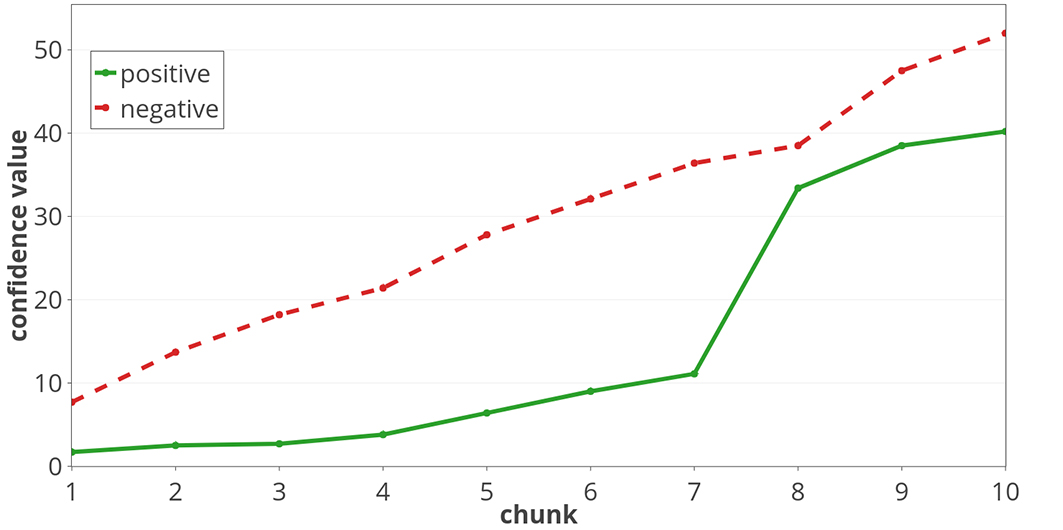
\includegraphics[width=\textwidth]{images/test_subject1914}
        \caption{Sujeto 1914, depresivo.}
        \label{fig:subjects_gv_d}
    \end{subfigure}
\caption{
\emph{Valores de confianza} acumulados a lo largo del tiempo (bloque a bloque).
Se muestran cuatro comportamientos típicos, ejemplificados cada uno con un sujeto distinto del conjunto de prueba.
% Accumulated confidence values over time (chunk by chunk).
% Four typical behaviors are shown, represented by these four subjects from the test set.
}
\label{fig:subject_cases}
\end{figure*}

Además, para comprender mejor los resultados obtenidos, otro aspecto importante a analizar es cómo  se llevó a cabo efectivamente la clasificación anticipada. 
Así, comenzaremos, primero, analizando la política más simple utilizada para decidir \emph{cuándo} clasificar positivamente a los sujetos. En la \autoref{fig:subject_cases} se muestran cuatro sujetos del conjunto de pruebas que ejemplifican cuatro tipos de comportamientos de clasificación anticipada que hemos detectado:
% Additionally, in order to better understand the good obtained results, another important aspect to analyze is how the early classification was actually carried out using the simplest policy to decide \emph{when} to positively classify subjects. In \autoref{fig:subjects_cases} are shown four subjects from the test set that illustrate four types of common classification behaviors we have detected:


\begin{itemize}
\item[(a)]
Desde el primer bloque de publicaciones en adelante, el valor de confianza de una de las clases,  ``no depresivo'' (negativo) en este caso, se mantiene siempre por encima y creciendo más rápidamente que el otro. En este ejemplo, correctamente, SS3 no pudo clasificar al sujeto como depresivo luego de haber leído todas sus publicaciones.
% from the first chunk on, the cumulative confidence value of one of the classes (negative in this case) stays above and always growing faster the other one. In this example, correctly, it was not possible to classify this subject as depressed after reading all its chunks.
\item[(b)]
Al igual que en el caso anterior, el valor de una clase (positiva en este caso) se mantiene siempre por encima de la otra, pero esta vez ambas crecen a un ritmo similar. En este ejemplo, el sujeto fue correctamente clasificado como depresivo.
% similar to the previous case, the value of one class (positive) stays always on top of the other one, but this time they both grow at a similar pace. The subject was correctly classified as depressed.
\item[(c)]
El valor de confianza negativo comienza siendo mayor que el positivo, pero a medida que se leen más publicaciones (en este caso, luego de leer el tercer bloque), el valor positivo comienza a crecer y continúa creciendo hasta superar al otro. En este ejemplo, el sujeto se clasificó correctamente como depresivo luego de que se leyera el quinto bloque de publicaciones.
% the accumulated negative confidence value starts being greater than the positive one, but as more chunks are read (specifically starting after reading the 3rd chunk), the positive value starts and stays growing until it exceeds the other one. In this case, this subject is classified as depressed after reading the 6th chunk.
\item[(d)]
Este ejemplo muestra un comportamiento similar al anterior. Sin embargo, si bien el valor positivo se acerca mucho al negativo, nunca alcanza a superarlo. Esto provocó que  el sujeto no haya podido ser clasificado correctamente como depresivo.
% this example has a behavior similar to the previous one, however, the positive value, despite getting very close at chunk 8, never exceeds the negative one, which leads to the subject 1914 being misclassified as negative.
\end{itemize}

\begin{figure}[t!] % [t]op; [h]ere; [p]age; [b]ottom; [r]ight; [l]eft
    \centering
    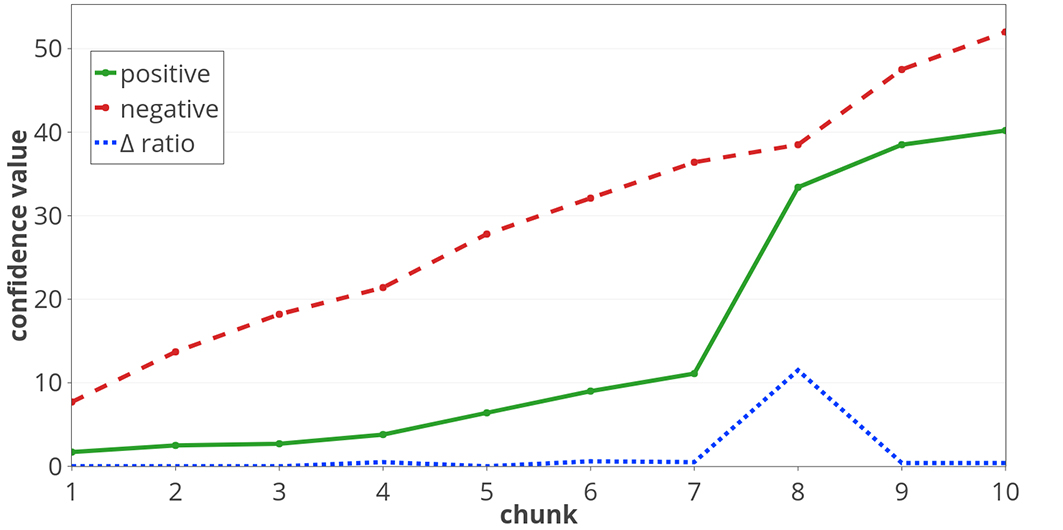
\includegraphics[width=120mm]{images/test_subject1914_slope}
    \caption{
    Sujeto 1914, depresivo.
    La tasa de cambio ($\Delta$) entre la curva positiva y negativa se muestra en azul (línea de puntos). Este cambio $\Delta$ fue el utilizado en la política del modelo $SS3^\Delta$.
    Notar que la línea azul tiene un pico en el bloque 8, lo que en este caso indica que el valor positivo ha crecido alrededor de 11 veces más rápido que el negativo, en ese punto.}
    % The ratio between the positive and the negative slope change ($\Delta$) is shown in blue dotted line. This ratio was used by the $\Delta$ policy.}
\label{fig:slope}
\end{figure}

La razón por la que se decidió implementar un segundo modelo, $SS3^\Delta$, fue para intentar evitar errores de clasificación similares al ejemplificado en (d). Es por esto que se decidió que su política también tenga en cuenta el crecimiento del \emph{valor de confianza} positivo en relación al negativo.
Más precisamente, como se puede ver en el \autoref{alg:classification_ss3slope}, y como se mencionó anteriormente, $SS3^\Delta$ clasifica un sujeto no sólo cuando el valor positivo supera al negativo, sino también cuando el valor positivo crece, al menos, cuatro veces más rápido que el negativo.
En la \autoref{fig:slope} se muestra nuevamente al sujeto 1914 (\autoref{fig:subjects_error_d}), pero esta vez se incluye información sobre los cambios en la pendiente de los valores.
Notar que este sujeto fue clasificado previamente como no depresivo porque el valor positivo nunca superó al negativo, pero utilizando esta nueva política, luego de leer el octavo bloque sí pudo ser clasificado correctamente.
% With the aim of avoiding cases of misclassification like in (d), we decided to implement the second classifier, SS3$^\Delta$, whose policy also takes into account the changes in both slopes.
% As it can be seen from \autoref{alg:classification_ss3slope} and as mentioned before, SS3$^\Delta$ additionally classifies a subject as positive if the positive slope changes, at least, four times faster than the other one.
% In \autoref{fig:slope} is shown again the subject 1914, this time including information about the changes in the slopes.
% Note that this subject was previously misclassified as not depressed because the accumulated positive value never exceeded the negative one, but by adding this new extra policy, this time it is correctly classified as positive after reading the 8th chunk\footnote{Note the peek in the blue dotted line pointing out that, at this point, the positive value has grown around 11 times faster than the negative one.}.

\begin{algorithm}[t!]
\small
\caption{\small
Algoritmo de clasificación anticipada utilizado por SS3$^\Delta$.
Donde \textproc{Clasificar-Bloque}($bloque$) es en realidad un alias de  \textproc{Clasificar-A-Nivel}($bloque$, 4) (dado en \autoref{alg:classification}).
}
  \label{alg:classification_ss3slope}
  \begin{algorithmic}[h]
  \Statex
  \Function{Clasificar-Sujeto}{$bloques$}
      \State \Input $bloques$, secuencia de bloques (de publicaciones)
      \State \LocalVariables $\overrightarrow{c}$, el \emph{vector de confianza} del sujeto
      \State \localvarsindent $\overrightarrow{\Delta c}$, el \emph{vector de confianza} de un bloque
      %\State
      \State $\overrightarrow{c} \gets \langle 0, 0\rangle$ $\rhd$ de la forma $\langle negativo, positivo\rangle$
      \For{$bloque$ \textbf{en} $bloques$}
          \State $\overrightarrow{\Delta c} \gets $\Call{Clasificar-Bloque}{$bloque$}
          \State $\overrightarrow{c} \gets \overrightarrow{c} + \overrightarrow{\Delta c}$ 
          %\State
          \If {$\frac{\overrightarrow{\Delta c}[1]}{\overrightarrow{\Delta c}[0]} > 4$ \Or $\overrightarrow{c}[1] > \overrightarrow{c}[0]$}
              \State \Return $positivo$ \Comment{clasificarlo como depresivo}
          \Else
              \State se requiere más evidencia
          \EndIf
      \EndFor
      %\State
      \State \Return $negativo$ \Comment{clasificarlo como no depresivo}
  \EndFunction
  \end{algorithmic}
\end{algorithm}

Como lo sugiere este último análisis, está claro que se puede obtener información útil del estudio de aquellos casos en los que el modelo no pudo clasificar correctamente a los sujetos. Con este objetivo en mente, también decidimos llevar a cabo un análisis de error, identificando así cuatro tipos de errores comunes, que podrían dividirse en dos grupos: los que, creemos, surgieron de un etiquetado incorrecto del conjunto de prueba y los que surgieron de un mal desempeño del clasificador en sí. En la \autoref{fig:subjects_error} se caracteriza cada tipo de error, nuevamente, utilizando cuatro sujetos del conjunto de prueba:
% From the previous analysis, it is clear that useful information can be obtained from the study of those cases where our approach was not able to correctly predict a class. With this goal in mind, we also carried out an error analysis and identified four common error cases which could be divided into two groups: those that arise from a bad labeling of the test set and those that arise from bad classifier performance. In \autoref{fig:subjects_error} we exemplify each case with one subject from the test set, described in more detail below:

\begin{figure*}[t!]
    \begin{subfigure}{0.5\textwidth}
        \centering
        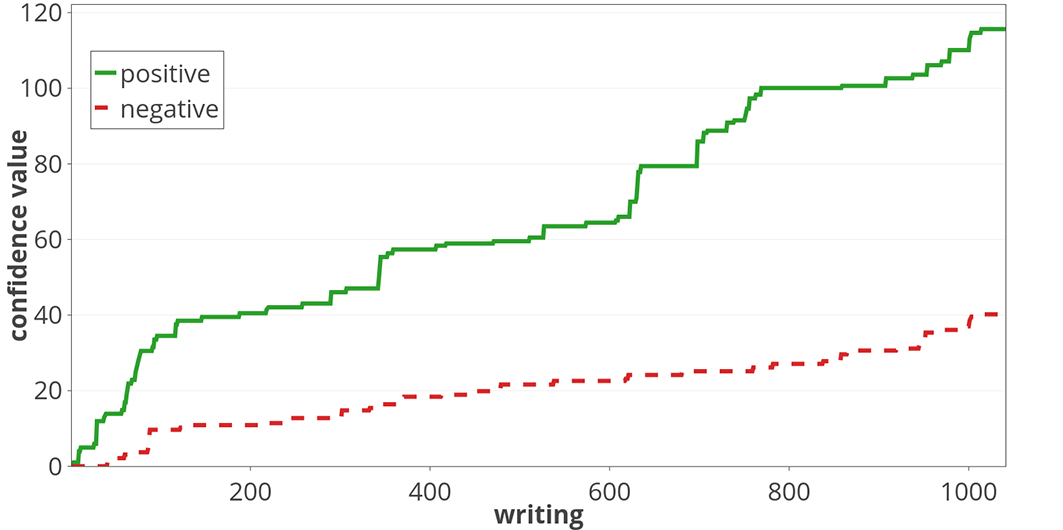
\includegraphics[width=\textwidth]{images/error1_test_subject834}
        \caption{Sujeto 834, no depresivo.}
        \label{fig:subjects_error_a}
    \end{subfigure}
    \begin{subfigure}{0.5\textwidth}
        \centering
        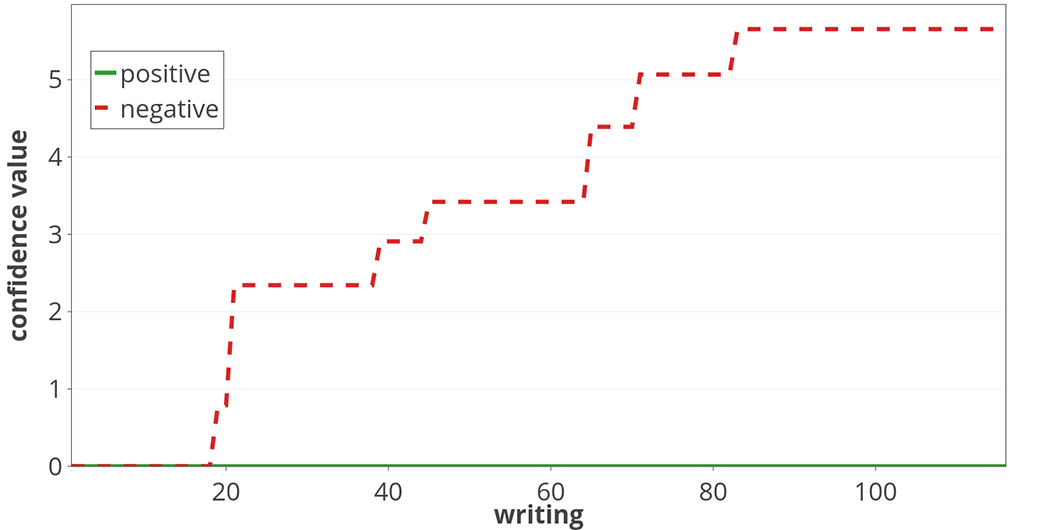
\includegraphics[width=\textwidth]{images/error2_test_subject1345}
        \caption{Sujeto 1345, depresivo.}
        \label{fig:subjects_error_b}
    \end{subfigure} \\
    \begin{subfigure}{0.5\textwidth}
        \centering
        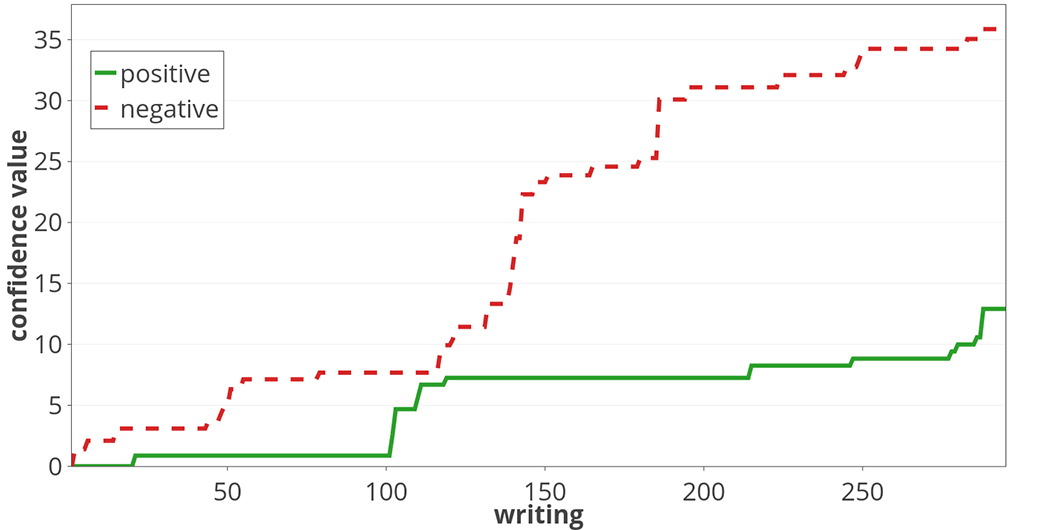
\includegraphics[width=\textwidth]{images/error3_test_subject2673}
        \caption{Sujeto 2673, depresivo.}
        \label{fig:subjects_error_c}
    \end{subfigure}
    \begin{subfigure}{0.5\textwidth}
        \centering
        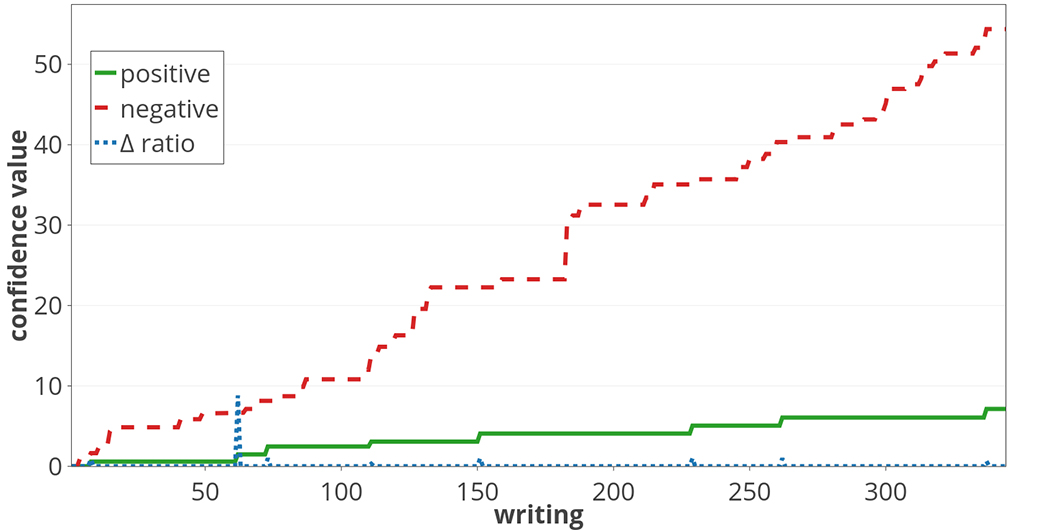
\includegraphics[width=\textwidth]{images/error4_test_subject748}
        \caption{Sujeto 748, no depresivo.}
        \label{fig:subjects_error_d}
    \end{subfigure}
\caption{
\emph{Valores de confianza} acumulados a lo largo del tiempo (publicación a publicación).
Se muestran cuatro casos comunes de error, cada uno ejemplificado con un sujeto del conjunto de prueba.
% Accumulated confidence values over time (writing by writing).
% Four common error cases, represented by these four subjects.
}
\label{fig:subjects_error}
\end{figure*}

\begin{itemize}
\item[(a)]
El sujeto se clasifica erróneamente como positivo ya que, efectivamente, el valor positivo superó y continuó superando al negativo. Tras un análisis manual de casos similares a éste, a menudo descubrimos que, al parecer, el clasificador no estaba equivocado al ``acumular confianza'' positiva, ya que a nuestro parecer, dichos sujetos eran efectivamente depresivos.\footnote{Por ejemplo, encontramos oraciones tales como la siguiente: ``Comencé la TCC (Terapia de conducta cognitiva) pero nunca la terminé. Es realmente difícil hacer TCC para depresión y ansiedad cuando además soy psicótico, gracias por darme apoyo moral, por así decirlo''.}
% the subject is misclassified as positive since the positive accumulated exceeded the negative one. When we manually analyzed cases like these we often found out that the classifier was correctly accumulating positive evidence since the users were, in fact, depressed.
% \footnote{We found sentences like this one: ``I did start CBT but I never finished it. It's really hard to do CBT for depression and anxiety when I'm psychotic, thank you for giving moral support so to speak''}.
\item[(b)]
En casos como éste, los sujetos se clasificaron erróneamente como negativos, debido a que SS3 no acumuló ninguna (o muy poca) evidencia positiva. Analizando manualmente las publicaciones de los sujetos, tampoco pudimos encontrar evidencia de que efectivamente fueran depresivos.\footnote{Los sujetos sólo hablaban sobre ciertos temas en general, tales como deportes, música, etc.}
% in cases like this one, subjects were misclassified as negative, since SS3 did not accumulate any (or very little) positive evidence. Manually analyzing the writings, we often could not find any positive evidence either, since subjects were talking about topics not related to depression (sports, music, etc.).
\item[(c)]
Hubo casos como el presentado aquí, en los que SS3 no pudo clasificar al sujeto como  depresivo,  debido a que el valor positivo acumulado no pudo superar el negativo, aun cuando en ocasiones pudo acercarse mucho. Notar que, cerca de la publicación número 100, el valor positivo se acerca mucho al negativo pero no alcanza a superarlo.\footnote{Quizás un ajuste más fino de los hiperparámetros podría superar este problema.}
% there were cases like this subject, in which SS3 failed to predict ``depression'' due to the accumulated positive value not being able to exceed the negative one even although, in some cases, it was able to get very close. Note that the positive value gets really close to the negative one at around the 100th writing.
% \footnote{Perhaps a finer tuning of hyper-parameters would overcome this problem.}
\item[(d)]
Este tipo de error se introdujo con la utilización de la política de $SS3^\Delta$.
En algunos casos, SS3 clasificó erróneamente a los sujetos como depresivos porque, si bien era cierto que el valor positivo cambió al menos 4 veces más rápido que el negativo, esta condición era verdadera debido a que el cambio negativo había sido muy pequeño (y no porque el positivo haya sido muy grande).
Por ejemplo, si el aumento del valor negativo fuese de $0.01$, un aumento positivo realmente pequeño, de al menos $0.04$, sería suficiente para disparar la decisión de ``clasificar como positivo''.\footnote{Quizás esto podría solucionarse al agregar una condición extra para controlar que el aumento positivo o negativo sea, al menos, mayor que alguna constante fija.}
En este ejemplo, este problema puede observarse en el pico azul punteado alrededor de la publicación 60, indicando que ``el valor positivo cambió cerca de 10 veces más rápido que el negativo''. En ese punto se clasifica erróneamente al sujeto como depresivo ya que el aumento de valor positivo fue, de hecho, muy pequeño.
% this type of error occurred only due to the addition of the slope ratio policy.
% In some cases, SS3 misclassified subjects as positive because, while it was true that the positive value changed at least 4 times more rapidly than the negative, the condition was mainly true only due to the negative change being very small.
% For instance, if the change of the negative confidence value was 0.01, a really small positive change of at least 0.04 would be enough to trigger the ``classify as positive'' decision.
% \footnote{Perhaps this could be fixed if we also request the positive or negative change to be, at least, bigger than a fixed constant (let us say 1) before applying the policy.}
% This problem can be detected in this subject by seeing the blue dotted peek at around the 60th writing, indicating that ``the positive slope changed around five times faster than the negative'' there, and therefore misclassifying it as positive. However, note that this positive change was in fact really small (less than 1). 
\end{itemize}


\begin{figure}[t!]
	\small
    \begin{subfigure}{\textwidth}
    	\centering
        \fbox{
        \begin{minipage}{0.9\textwidth}
        	\textbf{$\cdots$}\newline
        	\hlinew
            \textbf{Publicación 54 $\blacktriangleright$} I'm going to agree with everyone else and say you definitely need a lawyer. Get in touch with the[...]\newline
			\hlinew
			\textbf{Publicación 55 $\blacktriangleright$} \sethlcolor{dgreen_25}\hl{You don't mention what the fertility issue is (and you don't have to) but his feelings may stem fr[...]}\newline
            \hlinew
%            \textbf{Publicación 56 $\blacktriangleright$} Limited Experience . I am going through a divorce (yay, fun times) and while I don't think I'll [...]\newline
%            \hlinew
            \textbf{$\cdots$}\newline
            \hlinew
            \textbf{Publicación 59 $\blacktriangleright$} Thankfully I was able to realize that I was in a bad place and get help. My sister has been awesom[...]\newline
            \hlinew
            \textbf{Publicación 60 $\blacktriangleright$} \sethlcolor{dgreen_90}\hl{I have been seeing a therapist which I think is helping a little. Fact is, I was feeling really depressed[...]}\newline
            \hlinew
            \textbf{Publicación 61 $\blacktriangleright$} \sethlcolor{dgreen_50}\hl{My Wife Wants a Divorce . This will be long, sorry in advance. My wife told me shortly after the[...]}\newline
			\hlinew
            \textbf{Publicación 62 $\blacktriangleright$} the Earth Arena coming up I have: Zelnite x2 Dilma Ophelia For my last spot, should I use Miku[...]\newline
			\hlinew
            \textbf{$\cdots$}
        \end{minipage}
        }
        \caption{Historial del sujeto 9579 - nivel publicación\vspace{4mm}}
        \label{fig:subject9579_descriptive_a}
    \end{subfigure} \\
    \begin{subfigure}{0.5\textwidth}
        \centering
        \fbox{
        \begin{minipage}{0.9\textwidth}
			\sethlcolor{dgreen_25}\hl{I have been seeing a therapist which I think is helping a little}. \sethlcolor{dgreen_90}\hl{Fact is, I was feeling really depressed and wanting to kill myself}. I spent basically all of Feb in the hospital[...]
       	\end{minipage}
        }
        \caption{Publicación 60 - nivel oración}
        \label{fig:subject9579_descriptive_b}
    \end{subfigure}
    \begin{subfigure}{0.5\textwidth}
        \centering
        \fbox{
        \begin{minipage}{0.9\textwidth}
			I have been seeing a \sethlcolor{dgreen_50}\hl{therapist} which I think is helping a little. Fact is, I was \sethlcolor{dgreen_25}\hl{feeling} really \sethlcolor{dgreen_70}\hl{depressed} and wanting to kill \sethlcolor{dgreen_25}\hl{myself}. I spent basically all of Feb in the hospital[...]
       	\end{minipage}
        }
        \caption{Publicación 60 - nivel palabra}
        \label{fig:subject9579_descriptive_c}
    \end{subfigure}
    \caption{Esta figura muestra cómo se podría brindar una explicación visual del proceso de clasificación en la tarea abordada. Como mencionamos anteriormente, SS3 nos permite visualizar las razones detrás de la clasificación en diferentes niveles, en nuestro caso: (a) publicaciones, párrafos, (b) oraciones y/o (c) palabras. Cada uno de los segmentos está coloreado en relación al \emph{valor de confianza} positivo, real, obtenido en los experimentos realizados.}
% \caption{This figure shows how a visual description of the decision process could be given in this depression detection task. As we mentioned before, our framework allows us to analyze the reasons behind its classification decision, at different levels: (a) writings, (b) sentences and (c) words, etc. Each one of these blocks is painted proportionally to the real positive \emph{confidence values} we obtained after the experiments.}
\label{fig:subject9579_descriptive}
\end{figure}


Finalmente, creemos que es apropiado volver a examinar otra de las virtudes del modelo: \emph{su transparencia}.
Como se examinó anteriormente en la \autoref{sec:EC} del \autoref{cap3}, la mayoría de los clasificadores actúan como cajas negras, tanto tradicionales como modelos avanzados de \emph{aprendizaje profundo}.
% Esto es, el proceso de clasificación no se explica naturalmente por sí mismo y, por lo tanto, los humanos difícilmente pueden interpretar las razones detrás de la clasificación.
Sin embargo, como vimos y al igual que con cualquier otra tarea sensible o de detección de riesgo, con el fin de brindar ciertas garantías de confiabilidad, idealmente se espera que los modelos sean capaces de explicar o mostrar, de algún modo, las razones que lo llevaron a clasificar a los usuarios como tal.
% Sin embargo, como vimos, este es un aspecto esencial cuando la tarea involucra decisiones sensibles o de riesgo en las que, por lo general, personas reales están involucradas.
Así, en la  \autoref{fig:subject9579_descriptive} se muestra un ejemplo de lo que podría ser una explicación visual, dada por SS3, del proceso de clasificación para el sujeto 9579.\footnote{Notar que éste es el mismo sujeto que se utilizó anteriormente en el ejemplo mostrado al comienzo de este capítulo, en la \autoref{fig:subject9579_writings} de la \autoref{sec:classification_process}. Los lectores interesados pueden encontrar la relación entre la curva verde (positiva) mostrada allí y la intensidad del color de cada publicación mostrada en la \autoref{fig:subject9579_descriptive_a}.}
En este ejemplo se muestra en (a) un segmento del historial de publicaciones del sujeto, el cual ha sido coloreado en relación al \emph{valor de confianza} positivo asignado por SS3 ---lo que nos indica cuáles fueron las publicaciones involucradas, y en qué medida, en la decisión de clasificar al sujeto como positivo. Además, si un especialista quisiera analizar a su vez, digamos, la publicación 60 con más detalle, el mismo proceso podría utilizarse para los distintos niveles de la jerarquía que SS3 construye para clasificar, como por ejemplo se muestra en (b) y (c) para los niveles de oraciones y de palabras, respectivamente.
Vale la pena mencionar que debido a que este proceso de visualización se puede automatizar de una forma directa, utilizando los valores de los distintos \emph{vectores de confianza} de la jerarquía, hemos desarrollado una demo en línea, especialmente creada para este propósito, disponible en \url{http://tworld.io/ss3} ---por medio de esta demo los usuarios pueden probar ``en vivo y en directo'' a SS3 que, junto con el resultado de clasificación en sí mismo, brinda una explicación visual e interactiva de la clasificación.\footnote{De momento se encuentran disponibles dos modelos a probar, uno entrenado para el análisis de sentimientos en reseñas de películas y otro para clasificación temática.}
% Finally, we believe it is appropriate to highlight another of the highly desirable aspects of our Framework: its descriptive capacity.
% As mentioned previously in \autoref{sec:requeriments}, most of the classical and state-of-the-art classifiers act as black boxes (i.e. classification process is not self-explainable) and therefore humans are not able to naturally interpret the reasons behind the classification.
% However, this is a vital aspect, especially when the task involves sensitive or risky decisions in which, usually, people are involved. In \autoref{fig:subject9579_descriptive} is shown an example of a piece of what could be a visual description of the classification process for the subject 9579.
% \footnote{Note that this is the same subject who was previously used in the example shown in \autoref{fig:subject9579_writings}, in \autoref{sec:classification_process}. The interested readers could see the relation between the green/positive curve there and the color intensity of each writing shown in \autoref{fig:subject9579_descriptive_a}.}
% In this example, we show in (a) a painted piece of the subject's writings history that the system users could use to identify which were the writings involved, and to what degree, in the decision making (classification) process. if the user wanted to further analyze, let us say, the writing 60 in more details, the same process could be applied at two different lower levels, as shown in (b) and (c) for sentences and words respectively.
% It is worth mentioning that since this ``descriptive process'' can be easily automated we have developed an online live demo, especially built for this purpose, available at \href{http://tworld.io/ss3}{http://tworld.io/ss3}, in which users can try out a version of SS3 trained using tweets for topic classification (music, sports, etc.) that, along with the classification result, gives a visual description.


\subsection{Implicaciones y Consideraciones Clínicas}
% \subsection{Implications and Clinical Considerations}
\label{sec:implications_clinical}

Antes de finalizar este capítulo, dada la naturaleza del problema abordado, creemos importante examinar las implicaciones y consideraciones clínicas del trabajo realizado.

Como se resalta en Guntuku \emph{et al.} \cite{guntuku2017detecting}: ``Los métodos de detección automática pueden ayudar a identificar a personas depresivas o en riesgo a través del monitoreo pasivo, a gran escala, de las redes sociales, y en el futuro pueden complementar los procedimientos de detección existentes''.
En ese contexto, el modelo propuesto podría servir como un marco de trabajo con el que se podrían desarrollar sistemas, en un futuro, para el monitoreo pasivo a gran escala de las redes sociales que permita ayudar a detectar los primeros rastros de depresión analizando los patrones lingüísticos de los usuarios. Por ejemplo, dicho sistema podría filtrar usuarios presentando posibles candidatos, junto con información visual e interactiva, a profesionales de la salud mental para ser analizados manualmente. El aspecto de ``monitoreo pasivo a gran escala'' estaría respaldado, en principio, por la naturaleza paralelizable e incremental de SS3,\footnote{Sólo se requeriría almacenar un pequeño vector bidimensional, el \emph{vector de confianza}, por cada usuario.} mientras que la presentación de ``información visual e interactiva'' a los profesionales, por su naturaleza de caja blanca y la capacidad de explicar visualmente la clasificación.
Está claro que el trabajo abordado en esta tesis doctoral \emph{no persigue un objetivo de diagnóstico automático}, sino más bien el de brindar las bases para desarrollar, a futuro, herramientas de monitoreo complementarias a otros métodos bien establecidos dentro del estudio de la salud mental.
De hecho, varios problemas éticos y legales sobre la privacidad y protección de datos, y sobre cómo integrar efectivamente este tipo de métodos dentro de sistemas de salud, siguen siendo problemas abiertos de investigación~\cite{guntuku2017detecting}.
% As stated in \cite{guntuku2017detecting}: ``Automatic detection methods may help to identify depressed or otherwise at-risk individual through the large-scale passive monitoring of social media, and in the future may complement existing screening procedures''.
% In that context, our proposal is a potential tool with which systems could be developed in the future for large-scale passive monitoring of social media to help detecting early traces of depression by analyzing users' linguistic patterns, for instance, filtering users and presenting possible candidates, along with rich and interactive visual information, for mental health professionals to manually analyze them. The ``large-scale passive monitoring'' aspect would be supported by the incremental\footnote{Only one small vector, the \emph{confidence vector}, needs to be stored for each user.} and highly parallelized nature of SS3 while the ``rich and interactive visual information'' one by its white-box nature.
%is able to early detect certain linguistic patterns in the use of language of individual diagnosed with depression.
% It is clear that this work \emph{does not pursue a goal of autonomous diagnosis} but rather being a complementary tool to other well-established methods of mental health.
% As a matter of fact, several ethical and legal questions about data ownership and protection, and how to effectively integrate this type of approaches into systems of care are still open research problems \cite{guntuku2017detecting}.

El conjunto de datos utilizado en este trabajo tiene la ventaja de estar abierto al público y, si bien desempeñó un papel importante al impulsar el estudio de la relación entre el uso del lenguaje y el problema de detección de depresión, éste presenta algunas limitaciones desde un punto de vista metodológico/clínico.
Más allá del posible ``ruido'' introducido por el método utilizado para construir los grupos de usuarios  ``depresivos'' y ``no depresivos'', el conjunto de datos carece de cierta información adicional que podría ser muy valiosa para el problema de detección de depresión.
Por ejemplo, en otros conjuntos de datos, como el utilizado en De Choudhury \emph{et al.} \cite{de2013social}, además del texto propiamente dicho (tweets), también incluyen información muy valiosa y específica para este tipo de patología, como son los puntajes obtenidos en diferentes tests de depresión (\emph{CES-D} y \emph{BDI}), información sobre la red de contactos del usuario, índice de insomnio y patrones de publicación, entre otros.
Está claro que si hubiéramos tenido acceso a este tipo de información adicional, habría sido posible obtener, entre otros, una evaluación más confiable de los sujetos depresivos, el grado de severidad de la depresión, así como también la detección de algunos factores mediadores, como cambios de humor u ambientales, que podrían no ser directamente inferidos de las publicaciones de los usuarios.
Además, esta información también podría usarse para entrenar otros modelos e integrar sus predicciones con las obtenidas usando solamente información textual, por ejemplo, por medio del uso de métodos de ensamble de clasificadores.
% The dataset used in this task had the advantage of being publicly available and played an important role in determining how the use of language is related to the EDD problem. However, it exhibits some limitations from a methodological/clinical point of view. Beyond the potential ``noise'' introduced by the method to assess the ``depressed''/``non-depressed'' condition, it lacks some extra information that could be very valuable to the EDD problem.
% For instance, in other datasets, such as the one used in \cite{de2013social} for the detection of depression in social media (Twitter in this case), in addition to the text of the interactions (tweets), it was also available other extremely valuable information for this type of pathology such as the scores obtained in different depression tests (CES-D and BDI), information about the user's network of contacts and interaction behavior (such as an insomnia index and posting patterns), among others.
% It is clear that if we had had this additional information available, it would have been possible to obtain, among others, a more reliable assessment of depressive people, their severity levels of depression, and also to detect some mediating factors like environmental changes that could not be directly available in the users’ posts.
% Besides, this information could also be used to train other models and integrate their predictions with the ones obtained only using textual information by, for instance, using some late-fusion ensemble approach.

Finalmente, aunque la interpretación clínica de los resultados no se abordó en nuestro trabajo, es importante resaltar algunos puntos importantes.
En primer lugar, fue interesante observar que la mayoría de las 100 palabras identificadas por SS3, seleccionadas por mayor \emph{valor global}, se corresponden perfectamente a las categorías habitualmente identificadas en otros estudios más clínicos sobre depresión ---tales como palabras relacionadas a síntomas, tratamientos, divulgación/revelación (disclosure), relaciones/vida (relationships-life) \cite{ de2013social}.
Curiosamente, también notamos lo que podría llegar a ser una potencial nueva clase de palabras, aquellas vinculadas a los videojuegos multijugador en línea,\footnote{Como se puede ver en \autoref{fig:word_cloud}, por ejemplo, por las palabras vinculadas al popular videojuego Dota, como son ``Dota'', ``MMR'', ``Wards'', ``Mana'', ``Rune'', ``Gank'', ``Heroes'' y ``Viper''.}   sin embargo, un análisis serio de esto requeriría de un trabajo multidisciplinario con profesionales de la salud mental, lo que está fuera del alcance del presente trabajo.
Por otro lado, los gráficos que presentan los \emph{valores de confianza} acumulados a lo largo del tiempo, como son los de la \autoref{fig:subjects_error}, tienen la intención de mostrar cómo la evidencia léxica (aprendida desde los datos de entrenamiento y dada por la función $gv$) se acumula y varía con el tiempo ---y cómo ésta es usada por el modelo para decidir \emph{cuándo} se dispone de suficiente evidencia como para clasificarla.
Estos gráficos no deben interpretarse erróneamente como un intento de capturar cambios de humor u otros comportamientos típicos en personas depresivas.
Tenga en cuenta que, como se mencionó anteriormente, este tipo de información sí podría integrarse en nuestro modelo a través de métodos de ensamble de clasificadores, sin embargo, dado que no disponemos de un conjunto de datos que brinde este tipo de información, su implementación está más allá del alcance de este trabajo y será considerada como trabajo a futuro.
De hecho, creemos que la ampliación del modelo predictivo mediante la incorporación de este tipo de información vinculada a aspectos no lineales del comportamiento humano, como los cambios de humor, podría ayudar a capturar la variación de los síntomas de depresión a lo largo del tiempo.
Esto, por ejemplo, podría ayudar a detectar cuando los síntomas empeoran, como un medio para prevenir un posible suicidio o, si el sujeto ya está diagnosticado, para detectar cuando la terapia aplicada no está funcionando adecuadamente.
% Tener acceso a un conjunto de datos con este tipo de información de comportamiento permitiría, en el futuro, integrarlo al modelo mediante, por ejemplo, enfoques de ensamble de modelos.
% We believe that extending the predictive model by incorporating information related to non-linear aspects of human behavior, such as mood shifts, could help to capture when depression symptoms ``wax and wane''. This, for example, could help to detect when symptoms worsen as a means to prevent possible suicide or, if the subject is already diagnosed, to detect when applied therapy is not working. Having access to a dataset with this type of behavioral information would allow us in the future to integrate it into our EDD framework through, for example, a late-fusion ensemble approach.
\hfill$\square$

